\ifx\wholebook\relax \else
\documentclass[b5paper]{article}
\usepackage[nomarginpar
  %, margin=.5in
]{geometry}

\addtolength{\oddsidemargin}{-0.05in}
\addtolength{\evensidemargin}{-0.05in}
\addtolength{\textwidth}{0.1in}
\usepackage[en]{../prelude}

\setcounter{page}{1}

\begin{document}

\title{Solution search}

\author{Xinyu~LIU
\thanks{{\bfseries Xinyu LIU} \newline
  Email: liuxinyu95@gmail.com \newline}
  }

\maketitle
\fi

\markboth{Solution search}{Elementary Algorithms}

\ifx\wholebook\relax
\chapter{Solution search}
\numberwithin{Exercise}{chapter}
\fi

\def\includetikz{}

Computers enables people to search the solution for many problems: we build robot to search and pick the gadget in assembly lane; we develop car navigator to search the map for the best route; we make smart phone application to search the best shopping plan. This chapter is about the elementary lookup, matching, and solution search algorithms.

\section{$k$ selection problem}
\index{Selection algorithm}
A selection problem is to find the $k$-th smallest (or largest, $k > 0$) element in a collection $xs$ (list or array). The ordering is abstract, denoted as $\leq$. The intuitive method repeatedly finds the minimum for $k$ times. It takes $O(n)$ time to find the minimum, where $n = |xs|$ is the size. The total performance is bound to $O(kn)$. Alternatively, we can use heap to update, access the top element in $O(\lg n)$ time, hence find the $k$-th element in $O(k \lg n)$ time.

\be
top\ k\ xs = find\ k\ (\textit{heapify}\ xs)
\ee

Or in Curried form:

\be
top\ k\ = (find\ k) \circ \textit{heapify}
\label{eq:kth-heap1}
\ee

Where:

\be
\begin{array}{rcl}
find\ 1 & = & top \\
find\ k & = & (find\ (k - 1)) \circ pop
\end{array}
\label{eq:kth-heap2}
\ee

We can do it even better with the divide and conquer method. Pick an arbitrary element $p$ in $xs$, split $xs$ into $as$ and $bs$ with $p$ ($X = as \doubleplus [p] \doubleplus bs$), where $as = [x \gets xs, x \leq p]$ and $B = [x \gets xs, x > p]$. Let $m = |as|$ be the size of $as$, compare $m$ and $k$:

\begin{enumerate}
\item If $m = k - 1$, then $p$ is the $k$-th element;
\item If $m < k - 1$, the $k$-th element is in $as$, drop $bs $ and recursively search in $as$;
\item If $m > k - 1$, the $k$-th element is in $bs$, drop $as$ and recursively search the $(k-m)$-th element in $bs$.
\end{enumerate}

Reuse the \textit{part} function in quick sort (see \cref{eq:qsort-partition}):

\be
top\ k\ (x \cons xs) = \begin{cases}
  m = k - 1: & x, \text{where}\ m = |as|, (as, bs) = part\ (\leq x)\ xs \\
  m < k - 1: & top\ (k - m)\ bs \\
  \text{otherwise}: & top\ k\ as \\
\end{cases}
\ee

In ideal case, the split is balanced (the sizes of $as$ and $bs$ are almost same), halves the size every time. The performance is $O(n + n/2 + n/4 +...) = O(n)$. Same as the quick sort algorithm, the worst case happens when the partition is always unbalanced. The performance downgrades to $O(kn)$ or $O((n-k)n)$. In average case, we can find the $k$-th element in linear time. Most engineering practices in quick sort are applicable too, like the `media of three'\footnote{Blum, Floyd, Pratt, Rivest, and Tarjan developed a linear time algorithm in 1973\cite{CLRS}\cite{median-of-median}. Split the elements into groups, each has 5 elements at most. It gives $n/5$ medians. Repeat this to pick the median of median.}, and randomly pivot:

\begin{algorithmic}[1]
\Function{Top}{$k, xs, l, u$}
  \State \textproc{Exchange} $xs[l] \leftrightarrow xs[$ \Call{Random}{$l, u$} $]$ \Comment{Randomly select in $[l, u]$}
  \State $p \gets$ \Call{Partition}{$xs, l, u$}
  \If{$p - l + 1 = k$}
    \State \Return $xs[p]$
  \EndIf
  \If{$k < p - l + 1$}
    \State \Return \Call{Top}{$k, xs, l, p-1$}
  \EndIf
  \State \Return \Call{Top}{$k - p + l - 1, xs, p + 1, u$}
\EndFunction
\end{algorithmic}

We can change to return all the top $k$ elements (in arbitrary order), as below example program:

\lstset{frame = single}
\begin{Haskell}
tops _ [] = []
tops 0 _  = []
tops n (x:xs) | len == k = as
              | len <  n = as ++ [x] ++ tops (n - len - 1) bs
              | otherwise = tops n as
    where
      (as, bs) = partition (<= x) xs
      len = length as
\end{Haskell}

\section{Binary search}
\index{Binary search}

My high school teacher once played a `math magic'. He asked a student to pick a number from 0 to 1000 in mind. He asked 10 questions, then figured out that number based on the yes/no answers from the student. For example: is it even? is it prime? can it be divided by 3? and etc. If halves the numbers with every question, one can find any number within 1000 because $2^{10} = 1024 > 1000$. The question of whether it is even, perfectly halves numbers\footnote{There's a `mind reading' game in social network. One thinks about a person in mind. The AI robot asks 16 questions, and tells who that person is from the yes/no answers}. The game becomes not so interesting when the player guess like: 1000, high; 50, low; 750, low; 890, low; 990, correct! This is the {\em binary search} method. To find $x$ in an ordered sequence $A$, one firstly tries the middle point $y$. Done if $x = y$; if $x < y$, then drop the second half of $A$ as it's ordered; otherwise drop the first half. When $A = [\ ]$, then $x$ doesn't exist. $A$ need be ordered, I often see people are struggled with unordered data, confusing why the binary search does not work. {\em `Although the basic idea of binary search is comparatively straightforward, the details can be surprisingly tricky'} said Donald Knuth. Jon Bentley said most binary search implementations had error, including the one he gave in `{\em Programming pearls}'. He corrected the error after two decades\cite{Bentley}. Below is the binary search definition, where the lower and upper bounds of $A$ is $l$ and $u$ (exclude $u$).

\be
\textit{bsearch}\ x\ A\ (l, u) = \begin{cases}
  u < l: & \textit{Nothing} \\
  x = A[m]: & \textit{Just}\ m, \text{where}\ m =  l + \lfloor \dfrac{u - l}{2} \rfloor \\
  x < A[m]: & \textit{bsearch}\ x\ A\ (l, m - 1) \\
  \text{otherwise}: & \textit{bsearch}\ x\ A\ (m + 1, u) \\
\end{cases}
\ee

Or implement with loops:

\begin{algorithmic}[1]
\Function{Binary-Search}{$x, A, l, u$}
  \While{$l < u$}
    \State $m \gets l + \lfloor \dfrac{u - l}{2} \rfloor$ \Comment{avoid $\lfloor \dfrac{l+u}{2} \rfloor$ overflow}
    \If{$A[m] = x$}
      \State \Return $m$
    \EndIf
    \If{$x < A[m]$}
      \State $u \gets m - 1$
    \Else
      \State $l \gets m + 1$
    \EndIf
  \EndWhile
  \State Not found
\EndFunction
\end{algorithmic}

The performance of binary search is bound to $O(\lg n)$ because it halves $A$ every time. We can extend it to solve equation of monotone functions, for example $a^x = y$, where $a \leq y$, $a$ and $y$ are nature numbers. To find the integral $x$, exhaust $a^0, a^1, a^2, ...$, till $a^i = y$ or $a^i < y < a^{i+1}$ (no solution). If $a$ and $x$ are big numbers, it's expensive to compute $a^x$ in loops\footnote{One can reuse the result of $a^n$ to compute $a^{n + 1} = a a^n$. We consider generic monotone $f(n)$.}. Let's apply binary search. As $a^y \geq y$, we search in $[0, 1, ..., y]$. Function $f(x) = a^x$ is monotone, fix $x$, we examine the middle point: $x_m = \lfloor \dfrac{0 + y}{2} \rfloor$. If $a^{x_m} = y$, then $x_m$ is the solution; if $a^{m} < y$, we discard the range before $x_m$; otherwise discard the range after $x_m$. Both halve the search range. When the range becomes empty, it means no solution. Below is the implementation. Denote the monotone function as $f$, call $bsearch\ f\ y\ (0, y)$, where $f(x) = a^x$ to start. This method computes $f(x)$ for $O(\lg y)$ times, better than the exhaustive search.

\be
\textit{bsearch}\ f\ y\ (l, u) = \begin{cases}
  u < l: & \textit{Nothing}  \\
  f(m) = y: & \textit{Just}\ m, \text{where}\ m = \lfloor \dfrac{l + u}{2} \rfloor \\
  f(m) < y: & \textit{bsearch}\ f\ y\ (m + 1, u) \\
  f(m) > y: & \textit{bsearch}\ f\ y\ (l, m - 1) \\
  \end{cases}
\label{eq:bsearch}
\ee

\subsection{2D search}

Extend binary search to 2D or even higher dimension. Consider matrix $M$ of size $m \times n$. The elements in each row, column are ascending nature numbers as shown in \cref{fig:matrix-eg}. How to locate all elements equal to $z$? i.e. find all locations of $(i, j)$, such that $M_{i,j} = z$.

\be
[(x, y) | x \gets [1, 2,..., m], y \gets [1, 2,..., n], M_{x, y} = z]
\label{eq:bsearch-brute}
\ee

\begin{figure}[htbp]
 \centering
\[
\left [
  \begin{array}{ccccc}
    1 & 2 & 3 & 4 & ... \\
    2 & 4 & 5 & 6 & ... \\
    3 & 5 & 7 & 8 & ... \\
    4 & 6 & 8 & 9 & ... \\
    ... \\
  \end{array}
\right ]
\]
\caption{Each row, column is ascending.}
\label{fig:matrix-eg}
\end{figure}

Richard Bird used to interview students with this question\cite{fp-pearls}. Those who had programming experience at school tended to apply binary search. But it was easy to get stuck. One often checks the middle point $M_{\frac{m}{2}, \frac{n}{2}}$. If it is less than $z$, then drop the top-left rectangle; if greater than $z$ then drop the bottom-right rectangle, as shown in \cref{fig:bsearch-2D}, discard the shaded rectangle. Both cases lead to a L-shape search area, where one can't apply recursive search directly any more. Define the 2D search as: given $f(x, y)$, search integer solution $(x, y)$, such that $f(x, y) = z$. The matrix search is just a special case as:

\begin{figure}[htbp]
 \centering
 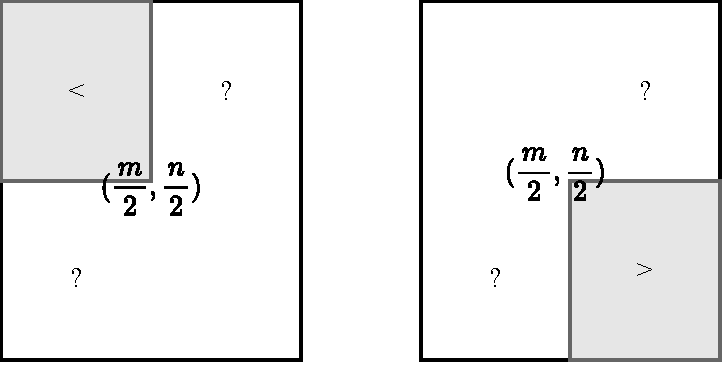
\includegraphics[scale=0.5]{img/binary-search-2d}
 \caption{Left: the middle point $< z$, all shaded rectangle $< z$; Right: the middle point $> z$, all shaded rectangle $> z$.}
 \label{fig:bsearch-2D}
\end{figure}

\[
f(x, y) = \begin{cases}
  1 \leq x \leq m, 1 \leq y \leq n: & M_{x, y} \\
  \text{otherwise}: & -1 \\
  \end{cases}
\]

\index{Saddle back search}
For monotone function $f(x, y)$, e.g., $f(x, y) = x^a + y^b$, where $a, b$ are nature numbers, the effective method is to search from the top-left, but not bottom-left\cite{saddle-back}. As shown in \cref{fig:saddleback-1}, start from $(0, z)$, for each location $(p, q)$, compare $f(p, q)$ and $z$:

\begin{enumerate}
\item If $f(p, q) < z$, since $f$ is monotone increasing, $f(p, y) < z$ for all $0 \leq y < q$. Drop all points in the vertical line segment ({\color{red}red});
\item If $f(p, q) > z$, then $f(x, q) > z$ for all $p < x \leq z$. Drop all points in the horizontal line segment ({\color{blue}blue});
\item If $f(p, q) = z$, then $(p, q)$ is a solution. Drop both line segments.
\end{enumerate}

Reduce the search rectangle line by line, every time drop a row, or a column, or both.

\begin{figure}[htbp]
 \centering
 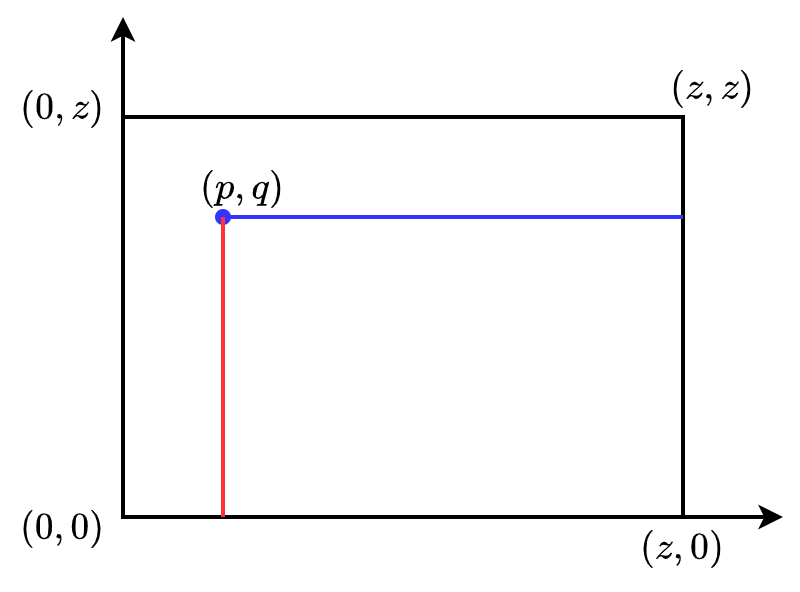
\includegraphics[scale=0.5]{img/saddle-back-start}
 \caption{Search from top-left.}
 \label{fig:saddleback-1}
\end{figure}

Define \textit{search} function as below, and pass the top-left corner: $search(f, z, 0, z)$

\be
\textit{search}\ f\ z\ p\ q\ =  \begin{cases}
  p > z\ \text{or}\ q < 0: & [\ ]   \\
  f(p, q) < z: & \textit{search}\ f\ z\ (p + 1)\ q  \\
  f(p, q) > z: & \textit{search}\ f\ z\ p\ (q - 1)  \\
  f(p, q) = z: & (p, q) : \textit{search}\ f\ z\ (p + 1)\ (q - 1) \\
  \end{cases}
\ee

Every time, at least one of $p$ and $q$ advances towards the bottom or right by one. It needs at most $2(z+1)$ steps. There are three best cases: (1) both $p$ and $q$ advance one a time, there are total $z + 1$ steps. As in \cref{fig:saddleback-1-cases} (a), all points in the diagonal line $(x, z-x)$ satisfy $f(x, z-x) = z$. It reaches to $(z, 0)$ in $z + 1$ steps; (2) move to the right horizontally till $p$ exceeds $z$. As in \cref{fig:saddleback-1-cases} (b), all points in the top horizontal line $(x, z)$ satisfy $f(x, z) < z$. It terminates after $z + 1$ steps; (3) move down vertically till $q$ becomes negative. As in \cref{fig:saddleback-1-cases} (c), all points in the left vertical line $(0, x)$ satisfy $f(0, x) > z$. It terminates after $z + 1$ steps; (d) is the worst case. If project all the horizontal sections in the search path to $x$ axis, all the vertical sections to $y$ axis, it gives the total steps of $2(z+1)$. This method improves the performance of exhaustive search from $O(z^2)$ to $O(z)$.

\begin{figure}[htbp]
 \centering
 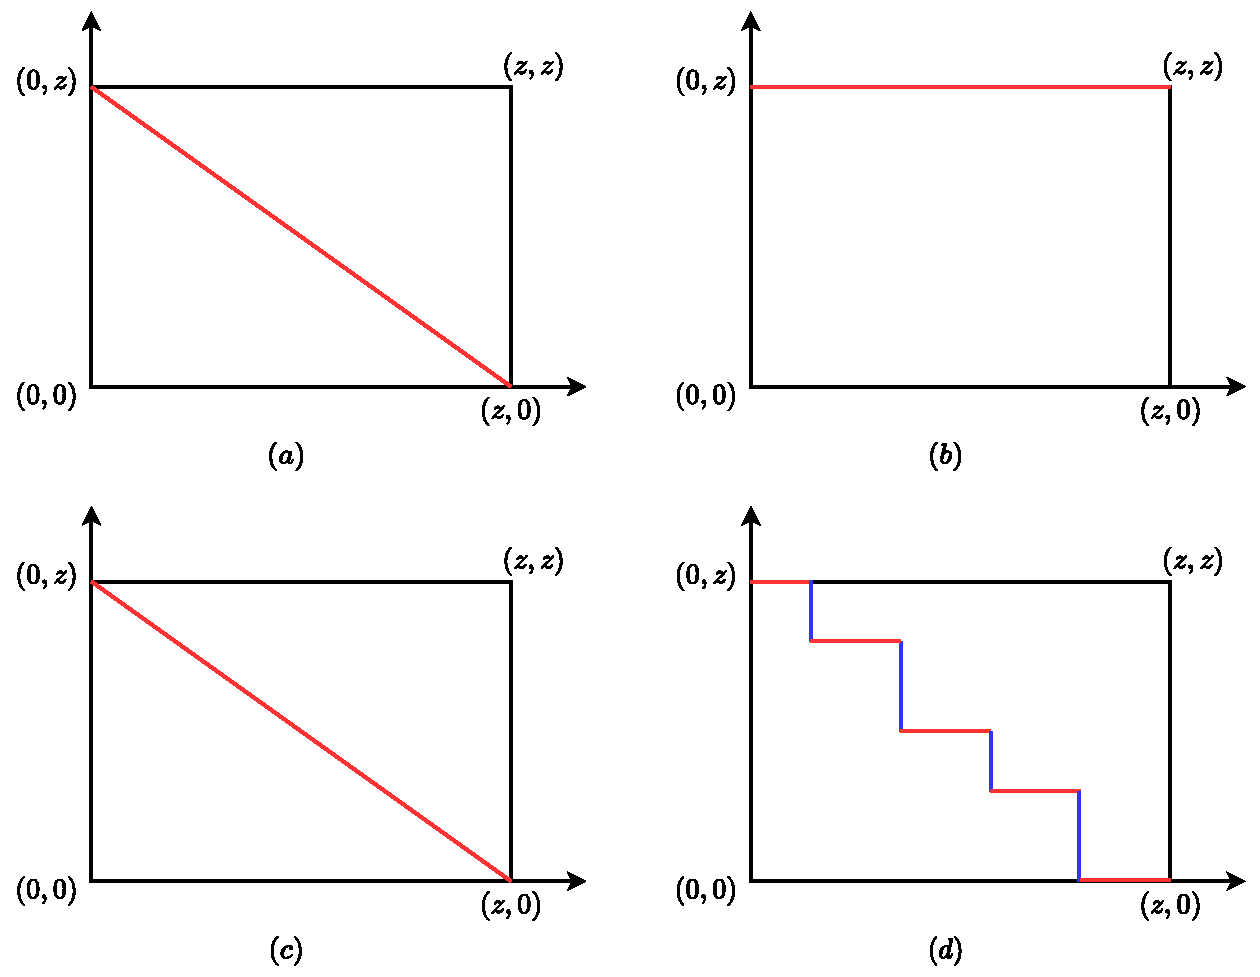
\includegraphics[scale=0.5]{img/saddle-back-paths}
 \caption{The best and worst cases.}
 \label{fig:saddleback-1-cases}
\end{figure}

This algorithm is called the {\em `saddle back'} search. The plot image of $f$ has the smallest bottom-left and the largest top-right. It looks like a saddle with two wings as shown in \cref{fig:saddleback-frame}. We can further reduce the search rectangle of $(0, z)- (z, 0)$. Since $f$ is monotone increasing, find the maximum $m$ along $y$ axis satisfying $f(0, m) \leq z$; find the maximum $n$ along $x$ axis satisfying $f(n, 0) \leq z$. Reduce the search rectangle to $(0, m) - (n, 0)$, as shown in \cref{fig:saddleback-2}.

\begin{figure}[htbp]
 \centering
 \includegraphics[scale=0.8]{img/saddleback-xx-yy}
 \caption{Plot of $f(x, y) = x^2 + y^2$.}
 \label{fig:saddleback-frame}
\end{figure}

\begin{figure}[htbp]
 \centering
 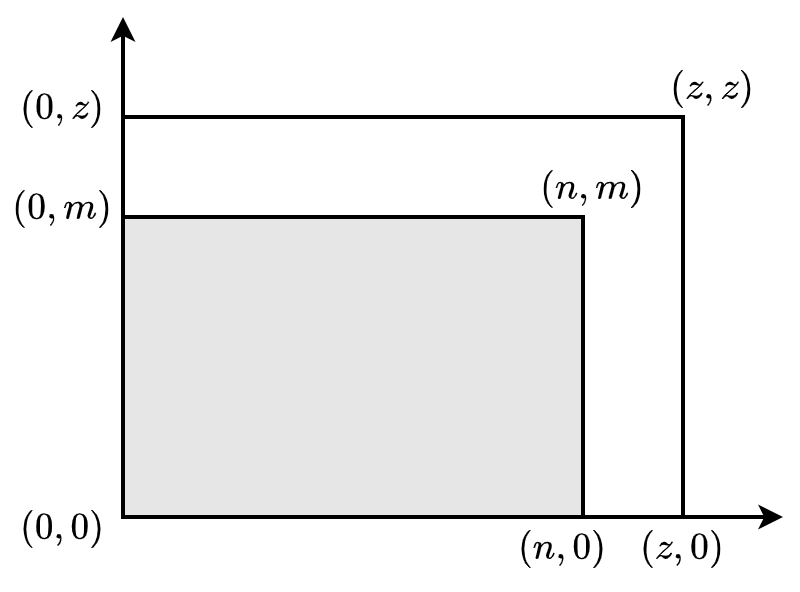
\includegraphics[scale=0.6]{img/saddle-back-area}
 \caption{Reduced search rectangle.}
 \label{fig:saddleback-2}
\end{figure}

\be
\begin{cases}
m & = \max\ \{0 \leq y \leq z, f(0, y) \leq z\} \\
n & = \max\ \{0 \leq x \leq z, f(x, 0) \leq z\}
\end{cases}
\ee

We can apply binary search to find $m$, $n$ (fix $x = 0$ to search $m$, fix $y = 0$ to search $n$). Modify \cref{eq:bsearch}, search $l \leq x \leq u$ satisfying $f(x) \leq y < f(x+1)$.

\be
\textit{bsearch}\ f\ y\ (l, u) = \begin{cases}
  u \leq l: & l \\
  f(m) \leq y < f(m + 1): & m, \text{where}\ m = \lfloor \dfrac{l + u}{2} \rfloor \\
  f(m) \leq y: & \textit{bsearch}\ f\ y\ (m + 1, u) \\
  f(m) > y : & \textit{bsearch}\ f\ y\ (l, m - 1)  \\
  \end{cases}
\label{eq:bsearch-general}
\ee

Then determine $m$, $n$ with binary search:

\be
\begin{cases}
m & = \textit{bsearch}\ (y \mapsto f(0, y))\ z\ (0, z) \\
n & = \textit{bsearch}\ (x \mapsto f(x, 0))\ z\ (0, z) \\
\end{cases}
\label{eq:bsearch-boundaries}
\ee

Finally, apply saddle back search in this smaller rectangle: $solve(f, z) = search(f, z, 0, \pmb{m})$

\be
\textit{search}\ f\ z\ p\ q\ =  \begin{cases}
  p > \pmb{n}\ \text{or}\ q < 0: & [\ ]   \\
  f(p, q) < z: & \textit{search}\ f\ z\ (p + 1)\ q  \\
  f(p, q) > z: & \textit{search}\ f\ z\ p\ (q - 1)  \\
  f(p, q) = z: & (p, q) : \textit{search}\ f\ z\ (p + 1)\ (q - 1) \\
  \end{cases}
\ee

We apply two rounds of binary search to find $m$, $n$, each round computes $f$ for $O(\lg z)$ times; The saddle back search computes $f$ for $O(m + n)$ times in the worst case; it's $O(\min(m, n))$ in the best case as below table. For functions like $f(x, y) = x^a + y^b$, $a, b \in \mathbb{N}$, the boundary $m$, $n$ are very small. The total performance is close to $O(\lg z)$.

\btab{|l|l|}
\hline
 & steps to compute $f$ \\
\hline
worst & $2 \log z + m + n$ \\
\hline
best & $2 \log z + \min(m, n)$ \\
\hline
\etab

As shown in \cref{fig:saddleback-drop}, for a point $(p, q)$ in rectangle $(a, b) - (c, d)$, if $f(p, q) \neq z$, we can only discard the shaded part ($\leq 1/4$). If $f(p, q) = z$, we can discard the bottom-left, top-right parts, and all points in row $p$ and column $q$ since $f$ is monotone. Hence reduce the search rectangle by 1/2. To find the point satisfying $f(p, q) = z$, we apply binary search along the horizontal or vertical central line. Because the performance is bound to $O(\lg |L|)$ for line $L$, we chose the shorter central line as shown in \cref{fig:saddleback-centerline}.

\begin{figure}[htbp]
 \centering
 \subcaptionbox{If $f(p, q) \neq z$, we can only drop the shaded area, the remaining is a 'L' shape.}{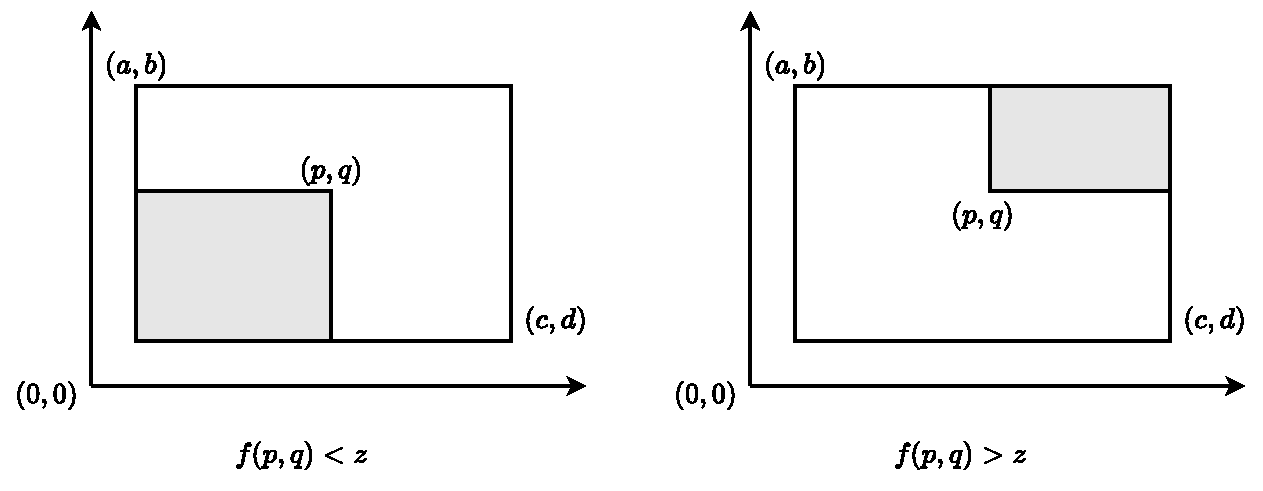
\includegraphics[scale=0.6]{img/saddleback-l-area}} \\
 \subcaptionbox{If $f(p, q) = z$, we can drop 1/2 rectangle.}{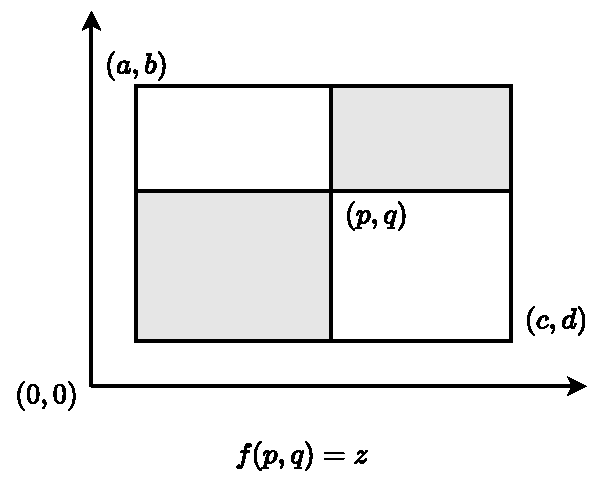
\includegraphics[scale=0.6]{img/saddleback-half-area}}
 \caption{Reduce the search rectangle.}
 \label{fig:saddleback-drop}
\end{figure}

\begin{figure}[htbp]
 \centering
 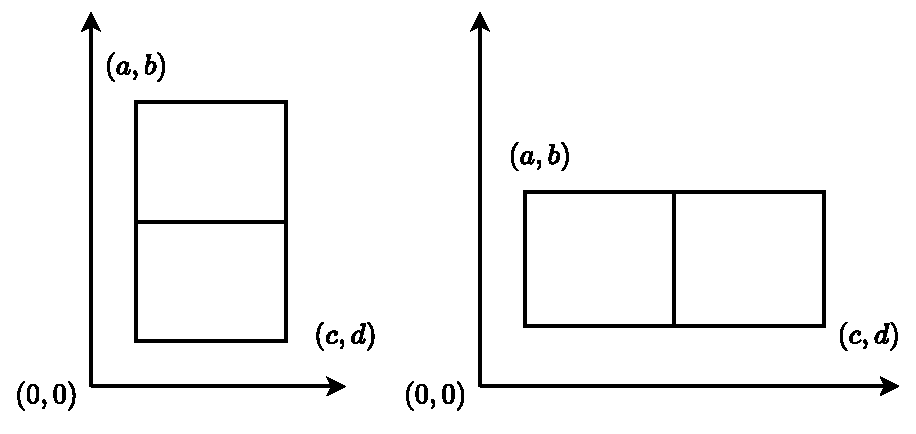
\includegraphics[scale=0.6]{img/saddleback-mid-line}
 \caption{Chose the shorter center line.}
 \label{fig:saddleback-centerline}
\end{figure}

If there is no point satisfying $f(p, q) = z$, find a point, such that $f(p, q) < z < f(p + 1, q)$ in the horizontal central line (or $f(p, q) < z < f(p, q + 1)$ for vertical central line). We can't discard all points in row $p$ and column $q$. In summary, we apply binary search along horizontal central line for the point: $f(p, q) \leq z < f(p + 1, q)$; or search the vertical central line for the point: $f(p, q) \leq z < f(p, q + 1)$. If all points in the line segment are $f(p, q) < z$, then return the upper bound; if all are $f(p, q) > z$, then return the lower bound. We discard half side in this case. Below is the improved saddle back search:

\begin{enumerate}
\item Apply binary search along the $x, y$ axes for the search rectangle $(0, m) - (n, 0)$;
\item For rectangle $(a, b) - (c, d)$, if the height > width, apply binary search along the horizontal central line; otherwise search along the vertical central line for the point $(p, q)$;
\item If $f(p, q) = z$, it is a solution. Recursively search rectangles $(a, b) - (p-1, q+1)$ and $(p+1, q-1) - (c, d)$;
\item If $f(p, q) \neq z$, recursively search the two rectangles and  a line section, either $(p, q+1) - (p, b)$ in \cref{fig:include-line} (a); or $(p+1, q) - (c, q)$ in \cref{fig:include-line} (b).
\end{enumerate}

\begin{figure}[htbp]
 \centering
 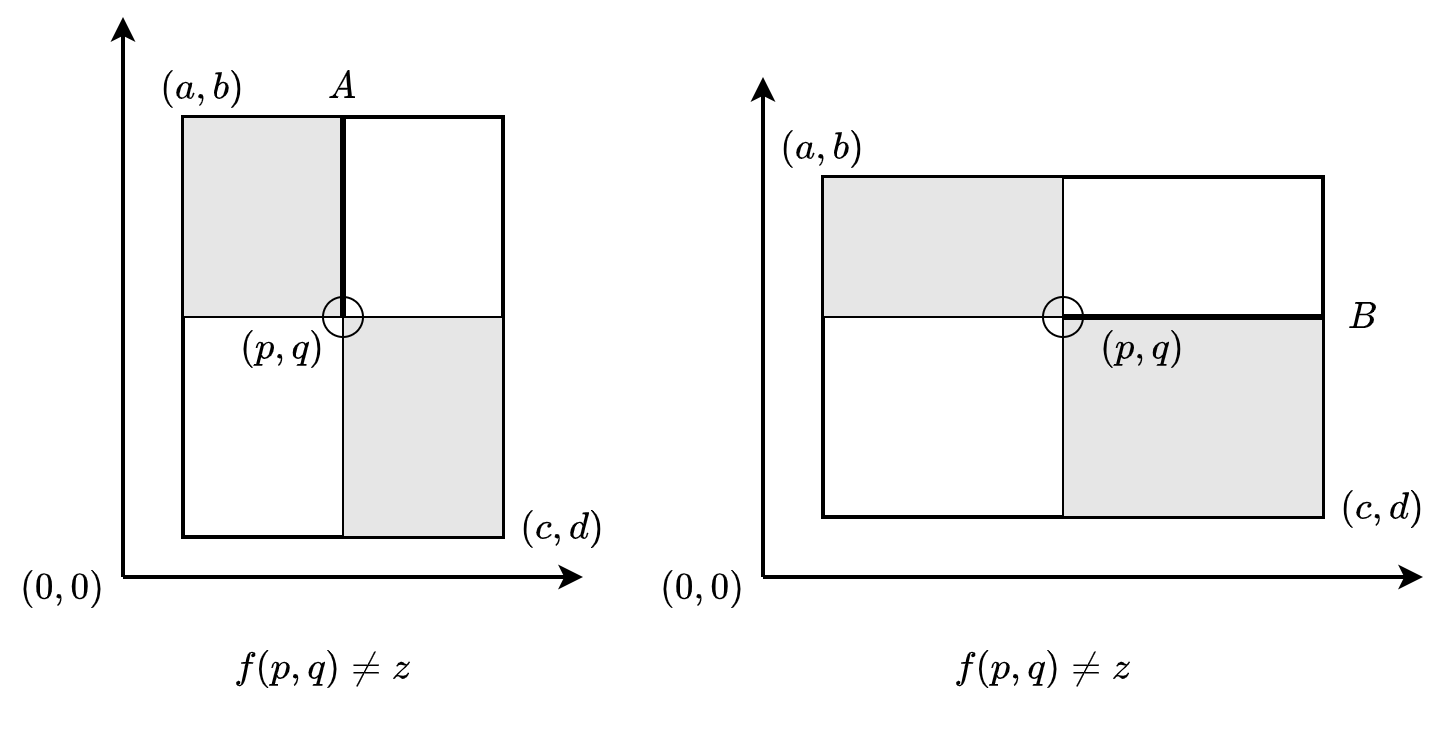
\includegraphics[scale=0.6]{img/saddleback-mid-line-inc}
 \caption{Recursively search the shaded parts, include the bold line  if $f(p, q) \neq z$.}
 \label{fig:include-line}
\end{figure}

\be
\textit{search}\ (a, b)\ (c, d) = \begin{cases}
  c < a\ \text{or}\ d < b: & [\ ] \\
  c - a < b - d: & \textit{csearch}  \\
  \text{otherwise}: & \textit{rsearch} \\
  \end{cases}
\ee

Where $csearch$ apply binary search to the horizontal central line for point $(p, q)$, such that $f(p, q) \leq z < f(p+1, q)$, as shown in \cref{fig:include-line} (a). If all function values are greater than $z$, then return the lower bound $(a, \lfloor \dfrac{b + d}{2} \rfloor)$. Drop the above side (include the central line) as shown in \cref{fig:saddleback-edge-cases} (a).

\begin{figure}[htbp]
 \centering
 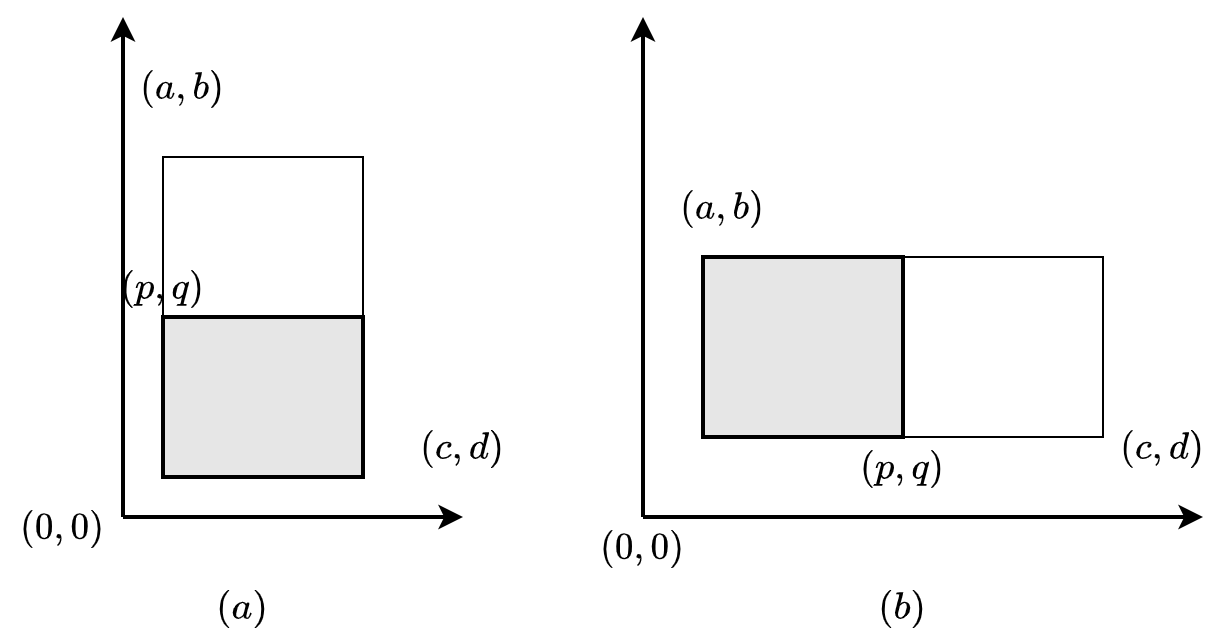
\includegraphics[scale=0.6]{img/saddleback-halve}
 \caption{Special case.}
 \label{fig:saddleback-edge-cases}
\end{figure}

Let

\[
\begin{cases}
q = \lfloor \dfrac{b + d}{2} \rfloor \\
p = \textit{bsearch}\ (x \mapsto f(x, q))\ z\ (a, c) \\
\end{cases}
\]

\be
\resizebox{\textwidth}{!}{\ensuremath{
\textit{csearch} = \begin{cases}
  f(p, q) > z: & \textit{search}\ (p, q - 1)\ (c, d)  \\
  f(p, q) = z: & \textit{search}\ (a, b)\ (p - 1, q + 1) \doubleplus [(p, q)] \doubleplus \textit{search}\ (p + 1, q - 1)\ (c, d) \\
  f(p, q) < z: & \textit{search}\ (a, b)\ (p, q + 1) \doubleplus \textit{search}\ (p + 1, q - 1)\ (c, d) \\
  \end{cases}
}}
\ee

Function $rsearch$ is symmetric along the vertical central line. Below example program implements the improved saddle back search:

\begin{Haskell}
solve f z = search f z (0, m) (n, 0) where
  m = bsearch (f 0) z (0, z)
  n = bsearch (\x -> f x 0) z (0, z)

search f z (a, b) (c, d)
       | c < a || b < d = []
       | c - a < b - d = let q = (b + d) `div` 2 in
           csearch (bsearch (\x -> f x q) z (a, c), q)
       | otherwise = let p = (a + c) `div` 2 in
           rsearch (p, bsearch (f p) z (d, b))
  where
    csearch (p, q)
        | z < f p q = search f z (p, q - 1) (c, d)
        | f p q == z = search f z (a, b) (p - 1, q + 1) ++
                 (p, q) : search f z (p + 1, q - 1) (c, d)
        | otherwise = search f z (a, b) (p, q + 1) ++
                 search f z (p + 1, q - 1) (c, d)
    rsearch (p, q)
        | z < f p q = search f z (a, b) (p - 1, q)
        | f p q == z = search f z (a, b) (p - 1, q + 1) ++
                 (p, q) : search f z (p + 1, q - 1) (c, d)
        | otherwise = search f z (a, b) (p - 1, q + 1) ++
                 search f z (p + 1, q) (c, d)
\end{Haskell}

As we halve the rectangle every time, we search $O(\lg (mn))$ rounds. We apply binary search along the central line for $(p, q)$, compute $f$ for $O(\lg (\min(m, n)))$ times. Let the time be $T(m, n)$ when search $m \times n$ rectangle. We have the following recursive equation:

\be
T(m, n) = \lg(min(m, n)) + 2 T(\dfrac{m}{2}, \dfrac{n}{2})
\ee

Suppose $m = 2^i > n = 2^j$, use telescope method:

\be
\begin{array}{rl}
T(2^i, 2^j) & = j + 2 T(2^{i-1}, 2^{j-1}) \\
            & = \displaystyle \sum_{k=0}^{i-1} 2^k(j - k) \\
            & = O(2^i(j-i)) \\
            & = O(m \lg (n/m))
\end{array}
\ee

Richard Bird proves this is asymptotically optimal by a lower bound of searching a given value in $m \times n$ rectangle \cite{fp-pearls}.

\begin{Exercise}\label{ex:binary-search}
\Question{Prove the performance of $k$-selection problem is $O(n)$ in average.}
\Question{To find the top $k$ element in $A$, we can search $x = \max\ (take\ k\ A), y = \min\ (drop\ k\ A)$. If $x < y$, then the first $k$ elements in $A$ is the answer; otherwise, we partition the first $k$ elements with $x$, partition the rest with $y$, then recursively find in sub-sequence $[a | a \gets A, x < a < y]$ for the top $k'$ elements, where $k' = k - |[a | a \gets A, a \leq x]|$. Implement this solution, and evaluate its performance.}
\Question{Find the `simplified' median of two sorted arrays $A$ and $B$ in $O(\lg (m + n))$ time, where $m = |A|, n = |B|$. The array index starts from 0. The simplified median is defined as $median(A, B) = C[\lfloor \dfrac{m + n}{2} \rfloor]$, where $C = merge(A, B)$ is the merged sorted array\footnote{In statistics, the median of an ascending data set $x$ with $n$ elements is defined as:
\[
median(x) = \begin{cases}
odd(n): & x[\frac{n + 1}{2}] \\
even(n): & \dfrac{1}{2}(x[\dfrac{n}{2}] + x[\dfrac{n}{2}+1]) \\
\end{cases}
\]
}.}
\Question{For the saddle back search, eliminate recursion, implement it in loops to update the boundaries.}
\Question{For 2D search, let the bottom-left be the minimum, the top-right be the maximum. if $z$ is less than the minimum or greater than the maximum, then no solution; otherwise cut the rectangle into 4 parts with a horizontal line and a vertical line crossed at the center. then recursive search in these 4 small rectangles. Implement this solution and evaluate its performance.}
\end{Exercise}

\begin{Answer}
\Question{Prove the performance of $k$-selection problem is $O(n)$ in average.

Refer to the performance analysis of quick sort in \cref{sec:quick-sort-big-o}.
}

\Question{To find the top $k$ element in $A$, we can search $x = \max\ (take\ k\ A), y = \min\ (drop\ k\ A)$. If $x < y$, then the first $k$ elements in $A$ is the answer; otherwise, we partition the first $k$ elements with $x$, partition the rest with $y$, then recursively find in sub-sequence $[a | a \gets A, x < a < y]$ for the top $k'$ elements, where $k' = k - |[a | a \gets A, a \leq x]|$. Implement this solution, and evaluate its performance.

\begin{algorithmic}[1]
\Procedure{Tops}{$k, A$}
  \State $l \gets 1$
  \State $u \gets |A|$
  \Loop
    \State $i \gets$ \Call{Max-At}{$A[l..k]$}
    \State $j \gets$ \Call{Min-At}{$A[k+1..u]$}
    \If{$A[i] < A[j]$}
      \State break
    \EndIf
    \State \textproc{Exchange} $A[l] \leftrightarrow A[j]$
    \State \textproc{Exchange} $A[k+1] \leftrightarrow A[i]$
    \State $l \gets$ \Call{Partition}{$A, l, k$}
    \State $u \gets$ \Call{Partition}{$A, k+1, u$}
  \EndLoop
\EndProcedure
\end{algorithmic}

The performance is $O(n)$ in average. Every loop, it takes linear time to locate the min $i$, max $j$. Then partition two rounds in linear time. If the partition is balanced, we discard half elements in average, hence the total time is bound to: $O(n + n/2 + n/4...) = O(n)$.
}
\Question{Find the `simplified' median of two sorted arrays $A$ and $B$ in $O(\lg (m + n))$ time, where $m = |A|, n = |B|$. The array index starts from 0. The simplified median is defined as $median(A, B) = C[\lfloor \dfrac{m + n}{2} \rfloor]$, where $C = merge(A, B)$ is the merged sorted array\footnote{In statistics, the median of an ascending data set $x$ with $n$ elements is defined as:
\[
median(x) = \begin{cases}
odd(n): & x[\frac{n + 1}{2}] \\
even(n): & \dfrac{1}{2}(x[\dfrac{n}{2}] + x[\dfrac{n}{2}+1]) \\
\end{cases}
\]
}.

We give two solutions. The first apply binary search in each array. Let $l = 0$ and $u = m$ be the lower and upper bounds respectively. We guess the median in $A$ is at index $i = \lfloor \frac{l + u}{2} \rfloor$. According to the definition of the simplified median, there are total $h = \lfloor \frac{m + n}{2} \rfloor$ elements before it. Where there are $i$ elements before $A[i]$ in $A$. If we guess right, then there are $j = h - i$ elements before $A[i]$ in $B$. If $B[j] \leq A[i] \leq B[j + 1]$ holds, then the guessed $A[i]$ is the median. Or update the boundaries $l$ or $u$ if we guessed too big or small. Below example program implements this solution:

\begin{Bourbaki}
K median([K] a, [K] b) {
    if a == [] then return b[length(b) / 2]
    if b == [] then return a[length(a) / 2]
    Int i = medianOf(a, b)
    return if i == -1 then return median(b, a) else a[i]
}

Int medianOf([K] a, [K] b) {
    Int l = 0, u = length(a)
    while l < u {
        var i = (l + u) / 2
        var j = (length(a) + length(b)) / 2  - i
        if j < 1 or j >= len(b) {
            if (j == 0 and a[i] <= b[0]) or
               (j == len(b) and b[j - 1] <= a[i]) then return i
            if j >= len(b) then l = i + 1 else u = i
        } else {
            if b[j - 1]  <= a[i] and a[i] <= b[j] then return i
            if a[i] < b[j - 1] then l = i + 1 else u = i
        }
    }
    return -1
}
\end{Bourbaki}

The second solution is to develop a generic function that looks for the $k$-th element. Assume $m \geq n$ (otherwise swap $A$ and $B$), If either array is empty, then return the $k$-th element of the other array. If $k = 1$, then return the smaller one between $A[0]$ and $B[0]$. Otherwise guess $j = min(k/2, n)$ and $i = k - j$, then check $A[i]$ and $B[j]$. If $A[i] < B[j]$, we drop all elements before $A[i]$ and after $B[j]$, then recursively find the $(k - i)$-th element of the remaining; otherwise, drop all before $B[j]$ and after $A[i]$, then recursively find the $(k-j)$-th one.

\begin{Bourbaki}
K median([K] xs, [K] ys) {
    Int n = length(xs), m = length(ys)
    return kth(xs, 0, n, ys, 0, m, (m + n) / 2 + 1)
}

K kth([K] xs, Int x0, Int x1, [K] ys, Int y0, Int y1, Int k) {
    if x1 - x0 < y1 - y0 then return kth(ys, y0, y1, xs, x0, x1, k)
    if x1 <= x0 then return ys[y0 + k - 1]
    if y1 <= y0 then return xs[x0 + k - 1]
    if k == 1 then return min(xs[x0], ys[y0])
    var j = min(k / 2, y1 - y0), i = k - j
    i = x0 + i, j = y0 + j
    if xs[i - 1] < ys[j - 1] then
        return kth(xs, i, x1, ys, y0, j, k - i + x0)
    else
        return kth(xs, x0, i, ys, j, y1, k - j + y0)
}
\end{Bourbaki}

We can't define the simplified median as the $m \in A \doubleplus B$, satisfying:

\[
|[y \gets A \doubleplus B, y < m]| - |[y \gets A \doubleplus B, y > m]| = 0, \pm 1
\]

Consider the counter example: $[0, 1, 2, 3, 3, 3, 3, 3, 5]$. It doesn't work even if we use $\leq$ and $\geq$.
}

\Question{For the saddle back search, eliminate recursion, implement it in loops to update the boundary.

\begin{algorithmic}[1]
\Function{Solve}{$f, z$}
  \State $p \gets 0, q \gets z$
  \State $S \gets \phi$
  \While{$p \leq z$ and $q \geq 0$}
    \State $z' \gets f(p, q)$
    \If{$z' < z$}
      \State $p \gets p + 1$
    \ElsIf{$z' > z$}
      \State $q \gets q - 1$
    \Else
      \State $S \gets S \cup \{(p, q)\}$
      \State $p \gets p + 1, q \gets q - 1$
    \EndIf
  \EndWhile
  \State \Return $S$
\EndFunction
\end{algorithmic}
}
\Question{For 2D search, let the bottom-left be the minimum, the top-right be the maximum. if $z$ is less than the minimum or greater than the maximum, then no solution; otherwise cut the rectangle into 4 parts with a horizontal line and a vertical line crossed at the center. then recursive search in these 4 small rectangles. Implement this solution and evaluate its performance.

\begin{algorithmic}[1]
\Procedure{Search}{$f, z, a, b, c, d$} \Comment{$(a, b)$: bottom-left $(c, d)$: top-right}
  \If {$z \leq f(a, b)$ or $f(c, d) \geq z$}
    \If{$z = f(a, b)$}
      \State record $(a, b)$ as a solution
    \EndIf
    \If{$z = f(c, d)$}
      \State record $(c, d)$ as a solution
    \EndIf
    \State \Return
  \EndIf
  \State $p \gets \lfloor \frac{a + c}{2} \rfloor$
  \State $q \gets \lfloor \frac{b + d}{2} \rfloor$
  \State \Call{Search}{$f, z, a, q, p, d$}
  \State \Call{Search}{$f, z, p, q, c, d$}
  \State \Call{Search}{$f, z, a, b, p, q$}
  \State \Call{Search}{$f, z, p, b, c, q$}
\EndProcedure
\end{algorithmic}

Let the time to search in rectangle of area $A$ be $T(A)$. We take $O(1)$ time to check whether $z \leq f(a, b)$ or $f(c, d) \geq z$, then divide into 4 smaller squares, i.e., $T(A) = 4 T(A/4) + O(c)$. We apply the master theorem, the complexity is $O(A) = O(m n)$, which is proportion to the area. It's essentially same as exhaustive search in the rectangle.
}
\end{Answer}

\section{The majority number}
\index{Boyer-Moor majority number}

People often vote and use computer to count the result. Suppose a candidate wins if and only if gets more than half votes. From the votes sequence A, B, A, C, B, B, D, ..., how to find the winner efficiently? We can use a map to count the result (see chapter 2)\footnote{There is a probabilistic sub-linear space counting algorithm published
in 2004, named as `Count-min sketch'\cite{count-min-sketch}.}.

\begin{lstlisting}[language = Bourbaki]
Optional<T> majority([T] xs) {
    Map<T, Int> m
    for var x in xs {
        if x in m then m[x]++ else mx[x] = 0
    }
    var (r, v) = (Optional<T>.Nothing, length(xs) / 2 - 1)
    for var (x, c) in m {
      if c > v then (r, v) = (Optional.of(x), c)
    }
    return r
}
\end{lstlisting}

The map is often implemented as a red-black tree or Hash table. For $m$ candidates, $n$ votes, below table gives the performance:

\btab{|l|l|l|}
\hline
map & time & space \\
\hline
self-balancing tree & $O(n \lg m)$ & $O(m)$ \\
\hline
Hash table & $O(n)$ & at least $O(m)$ \\
\hline
\etab

Define the element occurs over 50\% as the `majority'. Boyer and Moore developed an algorithm in 1980, which picks the majority element in one scan if there is with constant space\cite{boyer-moore-majority}. There is at most 1 majority. Repeat dropping two different elements till all remaining are same. If the majority exists, then it is the remaining. Start from the first vote, let the candidate be the winner so far with point 1. If the next one votes the same candidate, then add the winner point by 1, otherwise -1. The candidate won't be the winner when the point reduces to 0. We pick the candidate of the next vote as the new winner and go on. As shown in below table, if there exists majority $m$, then other candidates can't beat $m$. Otherwise if the majority doesn't exist (invalid vote result, no winner), then discard the recorded `winner'. We need another scan to valid the winner.

\btab{|l|l|l|}
\hline
winner & count & position \\
\hline
A & 1 & {\bf A}, B, C, B, B, C, A, B, A, B, B, D, B \\
A & 0 & A, {\bf B}, C, B, B, C, A, B, A, B, B, D, B \\
C & 1 & A, B, {\bf C}, B, B, C, A, B, A, B, B, D, B \\
C & 0 & A, B, C, {\bf B}, B, C, A, B, A, B, B, D, B \\
B & 1 & A, B, C, B, {\bf B}, C, A, B, A, B, B, D, B \\
B & 0 & A, B, C, B, B, {\bf C}, A, B, A, B, B, D, B \\
A & 1 & A, B, C, B, B, C, {\bf A}, B, A, B, B, D, B \\
A & 0 & A, B, C, B, B, C, A, {\bf B}, A, B, B, D, B \\
A & 1 & A, B, C, B, B, C, A, B, {\bf A}, B, B, D, B \\
A & 0 & A, B, C, B, B, C, A, B, A, {\bf B}, B, D, B \\
B & 1 & A, B, C, B, B, C, A, B, A, B, {\bf B}, D, B \\
B & 0 & A, B, C, B, B, C, A, B, A, B, B, {\bf D}, B \\
B & 1 & A, B, C, B, B, C, A, B, A, B, B, D, {\bf B} \\
\hline
\etab

\be
\begin{array}{rcl}
maj\ [\ ] & = & \nil \\
maj\ (x \cons xs) & = & scan\ (x, 1)\ xs \\
\end{array}
\ee

Where $scan$ is defined as:

\be
\begin{array}{rcl}
scan\ (m, v)\ [\ ] & = & m \\
scan\ (m, v)\ (x \cons xs) & = & \begin{cases}
  m = x: & scan\ (m, v + 1)\ xs \\
  v = 0: & scan\ (x, 1)\ xs \\
  \text{otherwise}: & scan\ (m, v - 1)\ xs \\
  \end{cases}
\end{array}
\ee

Or implement with fold (Curried form): $maj = foldr\ f\ (\nil, 0)$, where:

\be
f\ x\ (m, v) = \begin{cases}
  x = m: & (m, v + 1) \\
  v = 0: & (x, 1) \\
  \text{otherwise}: & (m, v - 1) \\
\end{cases}
\ee

Finally, verify the winner is the true majority:

\be
\textit{verify}\ m = \text{if}\ 2|filter\ (= m)\ xs| > |xs|\ \text{then}\ \textit{Just}\ m\ \text{else}\ \textit{Nothing}
\ee

Below is the corresponding iterative implementation:

\begin{algorithmic}[1]
\Function{Majority}{$A$}
  \State $c \gets 0, m \gets \nil$
  \For{each $a$ in $A$}
    \If{$c = 0$}
      \State $m \gets a$
    \EndIf
    \If{$a = m$}
      \State $c \gets c + 1$
    \Else
      \State $c \gets c - 1$
    \EndIf
  \EndFor
  \State $c \gets 0$
  \For{each $a$ in $A$}
    \If{$a = m$}
      \State $c \gets c + 1$
    \EndIf
  \EndFor
  \If{$c > \%50|A|$}
    \State \Return \textit{Just} $m$
  \Else
    \State \Return \textit{Nothing}
  \EndIf
\EndFunction
\end{algorithmic}

\begin{Exercise}\label{ex:majority-problem}
\Question{Extend to find $k$ majorities that occurs over $\lfloor n/k \rfloor$ in collection $A$, where $n = |A|$. Hint: Drop $k$ different elements every time, till the remaining is less than $k$ distinct candidates. Any $k$-majority (the one over $\lfloor n/k \rfloor$) must remain in the end.}
\end{Exercise}

\begin{Answer}[ref = {ex:majority-problem}]
\Question{Extend to find $k$ majorities that occurs over $\lfloor n/k \rfloor$ in collection $A$, where $n = |A|$.

\vspace{3mm}
We use a dictionary of $Map: T \mapsto Int$, where $T$ is the element type if $A$. It records the net-wins for candidate $a$. Start the dictionary from empty $\nil$. We scan $A$ while update the dictionary: $foldr\ maj\ \nil\ A$, where $maj$ is defined as:

\be
maj\ a\ m = \begin{cases}
  a \in m: & m[a] \gets m[a] + 1 \\
  |m| < k: & m[a] \gets 1 \\
  \text{otherwise}: & filter\ (b \mapsto m[b] \neq 0)\ \{b \mapsto m[b] - 1 | b \in m\}
  \end{cases}
\ee

For every $a$ in $A$, if $a \notin m$ (new to the dictionary), and the candidates in $m$ is less than $k$, we add $a$ to $m$ with one net-win vote: $m[a] \gets 1$; if $a \in m$, add the vote by 1: $m[a] \gets m[a] + 1$; otherwise, if there are already $k$ candidates, we reduce the vote by 1 for every one, and remove the candidate when the vote becomes 0.

We need verify the remaining candidates at last, whether the votes $> n/k$, let $m' = \{(a, 0) | a \in m\}$. Scan $A$ again: $foldr\ cnt\ m'\ A$, where $cnt$ is defined as:

\be
cnt\ a\ m' = \text{if}\ a \in m'\ \text{then}\ m'[a] \gets m'[a] + 1\ \text{else}\ m'
\ee

After scan, $m'$ records the votes for each candidate, we filter the true winners in: $keys\ (filter\ (> n/k)\ m')$.

\begin{Haskell}
majorities k xs = verify $ foldr maj Map.empty xs where
  maj x m | x `Map.member` m = Map.adjust (1+) x m
          | Map.size m < k = Map.insert x 1 m
          | otherwise = Map.filter (/=0) $ Map.map (-1 +) m
  verify m = Map.keys $ Map.filter (> th) $ foldr cnt m' xs where
    m' = Map.map (const 0) m
    cnt x m = if x `Map.member` m then Map.adjust (1+) x m else m
    th = (length xs) `div` k
\end{Haskell}

Below is the corresponding iterative implementation:

\begin{algorithmic}[1]
\Function{Maj}{$k, A$}
\State $m \gets \{\}$
\For{each $a$ in $A$}
  \If{$a \in m$}
    \State $m[a] \gets m[a] + 1$
  \ElsIf{$|m| < k$}
    \State $m[a] \gets 1$
  \Else
    \For{each $c$ in $m$}
      \State $m[c] \gets m[c] - 1$
      \If{$m[c] = 0$}
        \State \Call{Remove}{$c, m$}
      \EndIf
    \EndFor
  \EndIf
\EndFor
\For{each $c$ in $m$}
  \State $m[c] \gets 0$
\EndFor
\For{each $a$ in $A$} \Comment{verify}
  \If{$a \in m$}
    \State $m[a] \gets m[a] + 1$
  \EndIf
\EndFor
\State $r = [\ ], n \gets |A|$
\For{each $c$ in $m$}
  \If{$m[c] > \dfrac{n}{k}$}
    \State \Call{Add}{$c, r$}
  \EndIf
\EndFor
\State \Return $r$
\EndFunction
\end{algorithmic}
}
\end{Answer}

\section{Maximum sum of sub-vector}
\index{Maximum sum problem}

For vector $V$, define a range $V[i...j]$ as sub-vector, the sum of sub-vector is $S = V[i] + V[i+1] + ... + V[j]$. Empty $[\ ]$ is sub-vector of any vector with sum 0. How to find the maximum sum of a given vector $V$\cite{Bentley}? For example, in vector [3, -13, 19, -12, 1, 9, 18, -16, 15, -15], the sub-vector [19, -12, 1, 9, 18] gives the maximum sum of 35. If all elements are positive, then the max is the total sum. If all are negative, then the empty vector gives the max sum of 0. Below is the exhaustive search implementation:

\begin{algorithmic}[1]
\Function{Max-Sum}{$V$}
  \State $m \gets 0, n \gets |V|$
  \For{$i \gets 1$ to $n$}
    \State $s \gets 0$
    \For{$j \gets i$ to $n$}
      \State $s \gets s + V[j]$
      \State $m \gets $ \Call{Max}{$m, s$}
    \EndFor
  \EndFor
  \State \Return $m$
\EndFunction
\end{algorithmic}

The performance of exhaustive search is $O(n^2)$, where $n$ is the vector length. Similar to majority number algorithm, we scan the vector. For every position $i$, record the sum of sub-vector ends with $i$ as $A$, and the maximum sum so far as $B$. As shown in \cref{fig:max-sum-invariant}. $A$ is not necessarily equal to $B$. We maintain $B \leq A$ always hold. When $B + V[i] > A$, we replace $A$ with this greater value. When $B + V[i] < 0$, we reset $B$ to 0. Below table gives the steps when scan $[3, -13, 19, -12, 1, 9, 18, -16, 15, -15]$.

\begin{figure}[htbp]
 \centering
 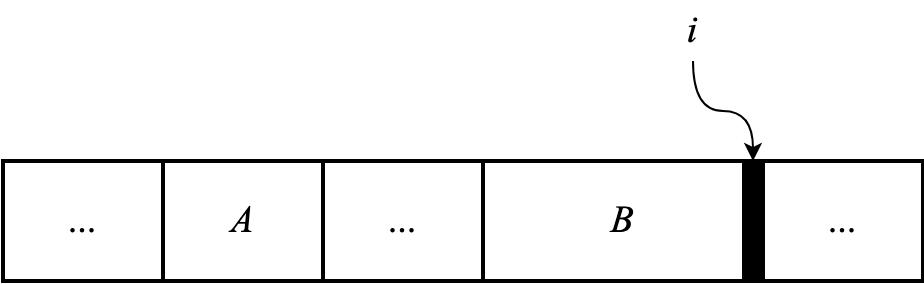
\includegraphics[scale=0.6]{img/max-sum}
 \caption{$A$: max sum so far; $B$: sum of the sub-vector ends with $i$.}
 \label{fig:max-sum-invariant}
\end{figure}

\btab{|l|l|r|}
\hline
max sum & max end at $i$ & yet to scan \\
\hline
0 & 0 & $[3, -13, 19, -12, 1, 9, 18, -16, 15, -15]$ \\
3 & 3 & $[-13, 19, -12, 1, 9, 18, -16, 15, -15]$ \\
3 & 0 & $[19, -12, 1, 9, 18, -16, 15, -15]$ \\
19 & 19 & $[-12, 1, 9, 18, -16, 15, -15]$ \\
19 & 7 & $[1, 9, 18, -16, 15, -15]$ \\
19 & 8 & $[9, 18, -16, 15, -15]$ \\
19 & 17 & $[18, -16, 15, -15]$ \\
35 & 35 & $[-16, 15, -15]$ \\
35 & 19 & $[15, -15]$ \\
35 & 34 & $[-15]$ \\
35 & 19 & $[\ ]$\\
\hline
\etab

\begin{algorithmic}[1]
\Function{Max-Sum}{$V$}
  \State $A \gets 0, B \gets 0, n \gets |V|$
  \For{$i \gets 1$ to  $n$}
    \State $B \gets $ \Call{Max}{$B + V[i], 0$}
    \State $A \gets $ \Call{Max}{$A, B$}
  \EndFor
  \State \Return $A$
\EndFunction
\end{algorithmic}

Or implement with fold (Curried form): $S_{max} = fst \circ foldr\ f\ (0, 0)$, where $f$ update the maximum sum so far:

\be
f\ x\ (S_m, S) = (S_m' = \max(S_m, S'), S' = \max(0, x + S))
\ee

\begin{Exercise}\label{ex:max-subsum}
\Question{Modify the solution that finds the max sum of sub-vector, returns the sub-vector of the maximum sum.}
\Question{Bentley gives a divide and conquer algorithm to find the max sum in $O(n \lg n)$ time\cite{Bentley}. Split the vector at middle, recursively find the max sum in two halves, and the max sum that crosses the middle. Then pick the greatest. Implement this solution.}
\Question{Find the sub-metrics in a $m \times n$ metrics that gives the maximum sum.}
\end{Exercise}

\begin{Answer}[ref = {ex:max-subsum}]
\Question{Modify the solution that finds the max sum of sub-vector, returns the sub-vector of the maximum sum.

If want to return the sub-list together with the maximum sum, we can maintain two pairs $P_m$ and $P$ during folding, each pair contains the sum and the sub-list $(S, L)$.

\blre
max_s & = & 1st \circ foldr\ f\ ((0, [\ ]), (0, [\ ])) \\
\text{where}: & & f\ x\ (P_m, (S, L)) = (P_m' = \max(P_m, P'), P' = \max((0, [\ ]), (x + S, x \cons L))) \\
\elre
}
\Question{Bentley gives a divide and conquer algorithm to find the max sum in $O(n \lg n)$ time\cite{Bentley}. Split the vector at middle, recursively find the max sum in two halves, and the max sum that crosses the middle. Then pick the greatest. Implement this solution.

\begin{algorithmic}[1]
\Function{Max-Sum}{$A$}
  \If{$A = \phi$}
    \State \Return 0
  \ElsIf{$|A| = 1$}
    \State \Return \Call{Max}{$0, A[1]$}
  \Else
    \State $m \gets \lfloor \frac{|A|}{2} \rfloor$
    \State $a \gets$ \textproc{Max-From}(\Call{Reverse}{$A[1...m]$})
    \State $b \gets$ \Call{Max-From}{$A[m+1...|A|]$}
    \State $c \gets$ \Call{Max-Sum}{$A[1...m]$}
    \State $d \gets$ \Call{Max-Sum}{$A[m+1...|A|$}
    \State \Return \textproc{Max}($a+b, c, d$)
  \EndIf
\EndFunction
\Statex
\Function{Max-From}{$A$}
  \State $sum \gets 0, m \gets 0$
  \For{$i \gets 1$ to $|A|$}
    \State $sum \gets sum + A[i]$
    \State $m \gets $ \Call{Max}{$m, sum$}
  \EndFor
  \State \Return $m$
\EndFunction
\end{algorithmic}

Consider the recursive equation: $T(n) = 2T(n/2) + O(n)$, from the master theorem, the performance is $O(n)$.
}

\Question{Find the sub-metrics in a $m \times n$ metrics that gives the maximum sum.

We start from the first row of the metrics, add a row per round $[M[1, *], M[2, *], ..., M[i, *]]$. Then sum the numbers in each column and convert it to a vector:

\[
V = \left [ \sum_{j=1}^i M[1, j], \sum_{j=1}^i M[2, j], ..., \sum_{j=1}^i M[n, j] \right ]
\]

Next use the $maxsum$ to find the max sum in vector $V$, and record the global maximum sum.

\begin{Haskell}
maxSum = maximum . (map maxS) . acc . rows where
    rows = init . tails              -- exclude the empty row
    acc = concatMap (scanl1 (zipWith (+))) -- accumulated sum along columns
    maxS = snd . (foldl f (0, 0))    -- max sum in a vector
    f (m, s) x = let m' = max (m + x) 0
                     s' = max m' s in (m', s')
\end{Haskell}

Where \texttt{tails} is defined in \cref{ex:list-tails}, \texttt{zipWith} is defined in \cref{sec:list-zipwith}, \texttt{concatMap} is defined in \cref{sec:list-concatmap}. The $scanl$ is similar to $foldl$, it records the result every time in a list. $scanl1$ is a special case of $scanl$, that the initial value is the first element.

\[
\begin{array}{rcl}
scanl1\ f [\ ] & = & [\ ] \\
scanl1\ f (x \cons xs) & = & scanl\ f\ x\ xs \\
\end{array}
\]

where

\[
\begin{array}{rcl}
scanl\ f\ q\ [\ ] & = & [q] \\
scanl\ f\ (x \cons xs) & = & q : scanl\ f\ (f\ q\ x)\ xs \\
\end{array}
\]

Below is the corresponding example program:

\begin{Bourbaki}
K maxsum2([[K]] m) {
    Int n = length(m), k = length(m[0]) // number of row, col
    K maxs = 0            // max so far
    for i = 0 to n - 1 {
        xs = [0] * k
        for j = i to n - 1 {
            xs = [x + y for (x, y) in zip(xs, m[j])]
            maxs = max(maxs, maxsum1(xs))
        }
    }
    return maxs
}

K maxsum1([K] xs) {
    K s = 0 // max so far
    K m = 0 // max end here
    for x in xs {
        m = max(m + x, 0)
        s = max(m, s)
    }
    return s
}
\end{Bourbaki}
}
\end{Answer}

\section{String matching}

\index{KMP} \index{Knuth-Morris-Pratt algorithm}
String matching is widely used in editor applications. We can use data structures like radix tree, prefix tree (see chapter 6) to search, or directly match the string as shown in \cref{fig:strstr}\footnote{Some programming environment provide match tool, like \texttt{strstr} in C library, \texttt{find} in C++ library, \texttt{indexOf} in Java library.}. We match a pattern $P$ in text $T$ character by character. At offset $s = 4$, the first 4 are same as shown in \cref{fig:strstr} (a), the 5th is `y' in $P$, but `t' in $T$. We stop here, add $s$ by 1 (move $P$ to right by 1), then restart matching `ananym' and `nantho...'. Actually, we can increase $s$ more than 1. The first two characters `an' happen to be the suffix of `anan'. We can add $s$ by 2 as shown in \cref{fig:strstr} (b). We reuse the information from the 4 matched characters, skip some positions. Knuth, Morris and Pratt develope an efficient matching algorithm from this idea \cite{kmp}, known as `KMP'. the initials of the three authors.

\begin{figure}[htbp]
 \centering
 \subcaptionbox{The offset $s = 4$, after matching $q=4$ characters, the 5th mismatches.}{\input{img/strstr.tex}} \\
 \subcaptionbox{Move $s = 4 + 2 = 6$.}{\input{img/kmp.tex}}
 \caption{Match `ananym' in `any ananthous ananym flower'.}
 \label{fig:strstr}
\end{figure}

Denote the first $k$ characters of text $T$ as $T_k$ (the $k$-character prefix of $T$). To shift $P$ to the right $s$ steps as far as possible, we need reuse the information of the matched $q$ characters. As shown in \cref{fig:kmp-fallback}, if we can shift $P$ ahead, there exists some $k$, such that the first $k$ characters are same as the last $k$ characters of $P_q$, i.e., the prefix $P_k$ is suffix of $P_q$. Define empty ``'' be both the prefix and suffix of any string, hence the minimum $k = 0$ always exists. We need find the maximum $k$ for the string that is both the prefix and suffix. Define the {\em prefix function} $\pi(q)$, that gives where to fallback when the $(q + 1)$-th character doesn't match\cite{CLRS}.

\begin{figure}[htbp]
 \centering
 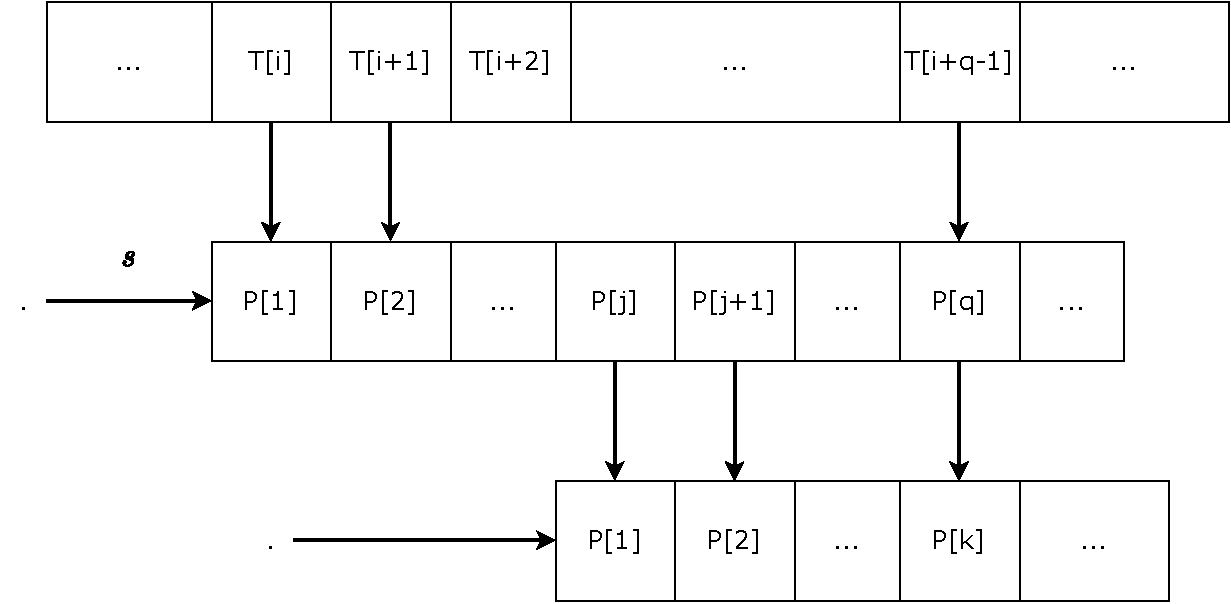
\includegraphics[scale=0.45]{img/kmp-fallback}
 \caption{$P_k$ is both the prefix and suffix of $P_q$.}
 \label{fig:kmp-fallback}
\end{figure}

\be
\pi(q) = \max \{ k | 0 \leq k < q, \text{and}\ P_k\ \text{is suffix of}\ P_q \}
\label{eq:prefix-function}
\ee

When match pattern $P$ against text $T$ from offset $s$, if fails after matching $q$ characters, we next look up $q' = \pi(q)$ to get a fallback position $q'$. Then retry to compare $P[q']$ with the text:

\begin{algorithmic}[1]
\Function{KMP}{$T, P$}
  \State $\pi \gets $ \Call{Build-Prefixes}{$P$}
  \State $n \gets |T|, m \gets |P|, q \gets 0$
  \For{$i \gets 1$ to $n$}
    \While{$q > 0$ and $P[q+1] \neq T[i]$}
      \State $q \gets \pi(q)$
    \EndWhile
    \If{$P[q+1] = T[i]$}
      \State $q \gets q + 1$
    \EndIf
    \If{$q = m$}
      \State position $i - m$ is a solution
      \State $q \gets \pi(q)$ \Comment{search further}
    \EndIf
  \EndFor
\EndFunction
\end{algorithmic}

The definition \cref{eq:prefix-function} is not practical to build $\pi(q)$. Let us pre-process $P$. If the first character doesn't match, then the longest prefix and suffix is empty: $\pi(1) = 0$, i.e., $P_k = P_0 = $ ``''. When scan the $q$-th character in $P$, the prefix function values $\pi(i)$, $i = 1, 2, ..., q-1$, are already known, and so far, the longest prefix $P_k$ is also the suffix of $P_{q-1}$. As shown in \cref{fig:kmp-prefix-func}, if $P[q] = P[k+1]$, we find a greater $k$, and increase $k$ by 1; otherwise, if $P[q] \neq P[k + 1]$, then lookup $\pi(k)$ and fallback to a shorter prefix $P_{k'}$, where $k' = \pi(k)$. Then compare the next character of this new prefix with the $q$-th character. Repeat this till $k$ becomes zero (empty string), or the $q$-th character matches. Below table gives the prefix function values of `ananym'. The $k$ column is the maximum satisfying \cref{eq:prefix-function}.

\begin{figure}[htbp]
 \centering
 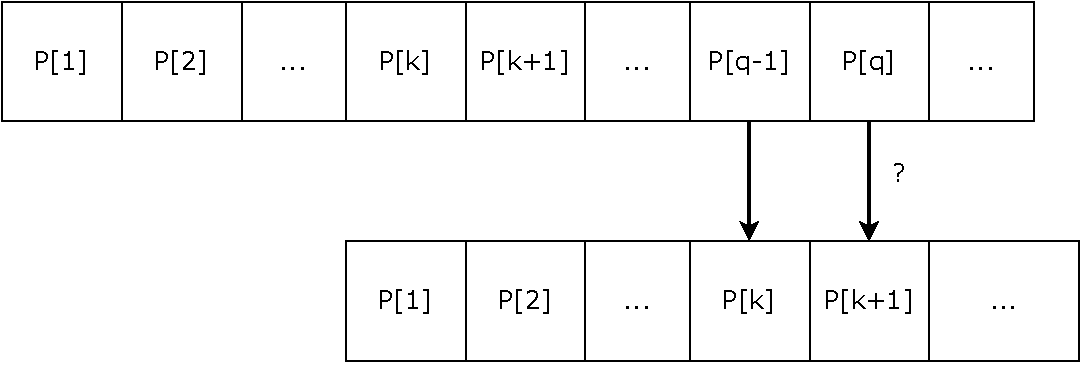
\includegraphics[scale=0.5]{img/kmp-prefix-func}
 \caption{$P_k$ is suffix of $P_{q-1}$, compare $P[q]$ and $P[k+1]$.}
 \label{fig:kmp-prefix-func}
\end{figure}

\btab{|c|r|c|l|}
\hline
$q$ & $P_q$ & $k$ & $P_k$ \\
\hline
1 & a & 0 & ``'' \\
2 & an & 0 & ``'' \\
3 & ana & 1 & a \\
4 & anan & 2 & an  \\
5 & anany & 0 & ``'' \\
6 & ananym & 0 & ``'' \\
\hline
\etab

\begin{algorithmic}[1]
\Function{Build-Prefixes}{$P$}
  \State $m \gets |P|, k \gets 0$
  \State $\pi(1) \gets 0$
  \For{$q \gets 2$ to $m$}
    \While{$k > 0$ and $P[q] \neq P[k+1]$}
      \State $k \gets \pi(k)$
    \EndWhile
    \If{$P[q] = P[k+1]$}
      \State $k \gets k + 1$
    \EndIf
    \State $\pi(q) \gets k$
  \EndFor
  \State \Return $\pi$
\EndFunction
\end{algorithmic}

The KMP algorithm builds the prefix function in amortized $O(m)$ time\cite{CLRS}, and matches the string in amortized $O(n)$ time, where $m = |P|$, $n = |T|$ are the lengths. The total amortized performance is $O(m + n)$, with additional $O(m)$ space to store the prefix function. Varies of pattern string $P$ don't impact the performance. Consider matching pattern `aaa...ab' (length of $m$) in string `aaa...a' (length of $n$). The $m$-th character doesn't match, we can only fallback by 1 repeatedly. The algorithm is still bound to linear time in this case.

%% \paragraph{Purely functional KMP algorithm}

%% Richard Bird presents a formal program deduction to KMP algorithm by using fold fusion law in chapter 17 of \cite{fp-pearls}.

\section{Solution search}

In early years of artificial intelligent, people developed methods to search solutions. Different from sequence and string matching, the solution may not directly exist among a set of candidates. We need construct the solution while try varies of options. Some problems are not solvable. Among the solvable ones, there can be multiple solutions. For example, a maze may have multiple ways out. We need find the optimal solution sometimes.

\subsection{DFS and BFS}
\index{DFS} \index{Deep-first search}
\label{sec:DFS-BFS}

DFS stands for deep-first search, and BFS stands for breadth-first search. They are typical graph search algorithms. We give some examples and skip the formal definition of graph.

\subsubsection{Maze}
\index{Maze problem}
Maze is a classic puzzle. There is saying: always turn right. However, it ends up loops as shown in \cref{fig:maze-loop}. The decision matters when there are multiple ways. In fairy tales, one takes some bread crumbs in a maze. Select a way, leave a piece of bread. If later enters a died end, then goes back to the last place through the bread crumbs. then goes to another way. Whenever sees bread crumbs left, one knows he visited it before. Then goes back and tries a different way. Repeats the `try and check' step, one will either find the way out, or go back to the starting point (no solution). We use $m \times n$ matrix to define a maze, each element is 0 or 1, means there is a way or not. Below matrix defines the maze in \cref{fig:maze-loop} (b):

\begin{figure}[htbp]
 \centering
 \subcaptionbox{Maze}{\includegraphics[scale=0.3]{img/maze}}
 \subcaptionbox{Loop when keep turning right.}{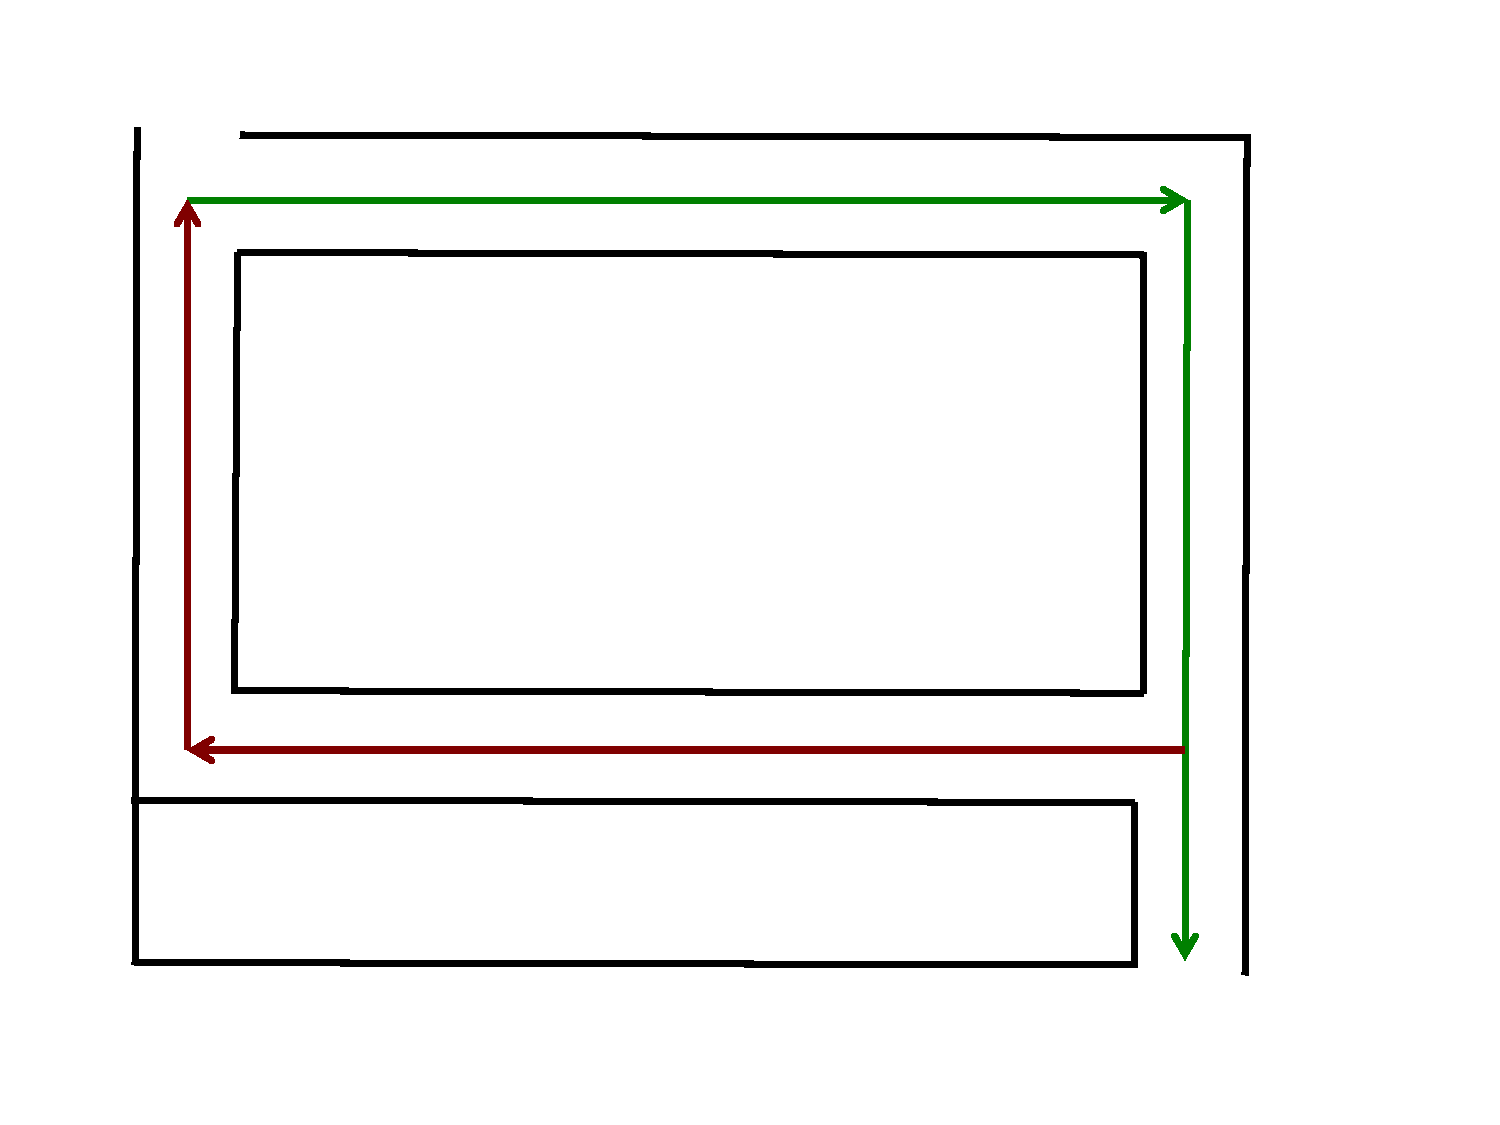
\includegraphics[scale=0.22]{img/maze-loop}}
 \caption{Maze}
 \label{fig:maze-loop}
\end{figure}

\[
\begin{matrix}
0 & 0 & 0 & 0 & 0 & 0 \\
0 & 1 & 1 & 1 & 1 & 0 \\
0 & 1 & 1 & 1 & 1 & 0 \\
0 & 1 & 1 & 1 & 1 & 0 \\
0 & 1 & 1 & 1 & 1 & 0 \\
0 & 0 & 0 & 0 & 0 & 0 \\
1 & 1 & 1 & 1 & 1 & 0
\end{matrix}
\]

Given a start point $s=(i, j)$, a destination $e=(p, q)$, we need find all paths from $s$ to $e$. We first examine all points connected with $s$. For every such point $k$, recursively find all paths from $k$ to $e$. Then prepend path $s$-$k$ to every path from $k$ to $e$. We need leave some `bread crumbs' to avoid looping. We use a list $P$ to record all visited points. Look it up and only try new ways.

\be
\textit{solveMaze}\ M\ s\ e = \textit{solve}\ s\ [[\ ]]
\label{eq:solve-maze-reversed}
\ee

Where:

\be
\textit{solve}\ s\ P = \begin{cases}
  s = e: & map\ (\textit{reverse} \circ (s:))\ P \\
  \text{otherwise}: & \textit{concat}\ [\textit{solve}\ k\ (map\ (s:)\ P) | k \gets adj\ s, k \notin P] \\
  \end{cases}
\ee

The paths in $P$ are reversed, we \textit{reverse} the result back finally. Function $adj\ p$ enumerates adjacent points to $p$:

\be
\begin{array}{ll}
adj\ (x, y) = [(x', y') \gets & [(x-1, y), (x+1, y), (x, y-1), (x, y+1)], \\
 & 1 \leq x' \leq m, 1 \leq y' \leq n, M_{x' y'} = 0] \\
\end{array}
\ee

This essentially `exhaustive searches' all possible paths. We only need one way out. We need some data structure serves for the 'bread crumbs', recording the previous decisions. We always search on top of the latest decision. We can use stack to realize the last-in, first-out order. The stack starts from $[s]$. Pop $s$ out and find all connected points of $a, b, ...$, push the new paths $[a, s]$, $[b, s]$ to the stack. Next pop $[a, s]$ out, examine all points connected to $a$. Then push new paths consist of 3 steps to the stack. Repeat this. The stack records paths in reversed order: from the farthest place back to the starting point, as shown in \cref{fig:dfs-stack}. If the stack becomes empty, we've tried all ways, and terminate the search; otherwise, we pop a path, expand to new adjacent points, and push the new paths back.

\begin{figure}[htbp]
 \centering
 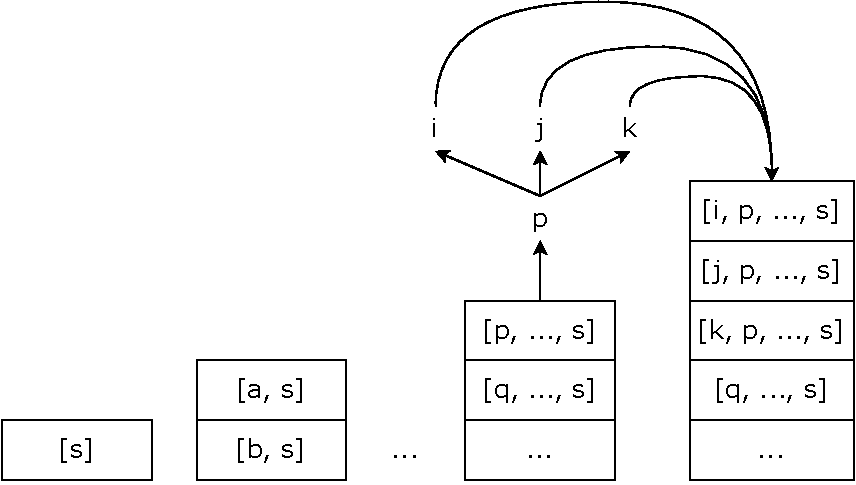
\includegraphics[scale=0.5]{img/dfs-stack}
 \caption{Search with a stack}
 \label{fig:dfs-stack}
\end{figure}

\be
\textit{solveMaze}\ M\ s\ e = \textit{solve}\ [[s]]
\ee

Where:

\be
\begin{array}{rcl}
\textit{solve}\ [\ ] & = & [\ ] \\
\textit{solve}\ ((p \cons ps) \cons cs) & = & \begin{cases}
  c = e: & \textit{reverse}\ (p \cons ps) \\
  ks = [\ ]: & \textit{solve}\ cs, \text{where}\ ks = filter\ (\notin ps)\ (adj\ p) \\
  ks \neq [\ ]: & \textit{solve}\ ((map\ (:p \cons ps)\ ks) \doubleplus cs)
  \end{cases}
\end{array}
\ee

Below is the iterative implementation:

\begin{algorithmic}[1]
\Function{Solve-Maze}{$M, s, e$}
  \State $S \gets [s], L = [\ ]$
  \While{$S \neq [\ ]$}
    \State $P \gets$ \Call{Pop}{$S$}
    \State $p \gets$ \Call{Last}{$P$}
    \If{$e = p$ }
      \State \Call{Add}{$L, P$}   \Comment{find a solution}
    \Else
      \For{each $k$ in \Call{Adjacent}{$M, p$}}
        \If{$k \notin P$}
          \State \Call{Push}{$S, P \doubleplus [k]$}
        \EndIf
      \EndFor
    \EndIf
  \EndWhile
  \State \Return $L$
\EndFunction
\end{algorithmic}

Each step tries 4 options (up, down, left, and right) through the backtrack. It seems the performance is $O(4^n)$, where $n$ is the length of the path. The actual time won't be so large because we skip the visited places. In the worst case, we traverse all the reachable points {\em exactly once}. Hence the time is bound to $O(n)$, where $n$ is the
number of connected points. We need additional $O(n^2)$ space for the stack.

\begin{Exercise}\label{ex:dfs-maze}
\Question{Modify the implementation with stack, find all ways to the maze.}
\end{Exercise}

\begin{Answer}[ref = {ex:dfs-maze}]
\Question{Modify the implementation with stack, find all ways to the maze.

\begin{Haskell}
dfsSolveAll m from to = map reverse $ solve [[from]] [] where
    solve [] ss = ss
    solve (c@(p:path):cs) ss
        | p == to = solve cs (c:ss) -- find a solution, go on search
        | otherwise = let os = filter (`notElem` path) (adjacent p) in
                          if os == [] then solve cs ss
                          else solve ((map (:c) os) ++ cs) ss
    adjacent (x, y) = [(x', y') |
           (x', y') <- [(x-1, y), (x+1, y), (x, y-1), (x, y+1)],
           inRange (bounds m) (x', y'), m ! (x', y') == 0]
\end{Haskell}

The corresponding imperative program:

\begin{Bourbaki}
[[(Int, Int)]] solve([[Int]] m, (Int, Int) src, (Int, Int) dst) {
    [[(Int, Int)]] stack = [[src]]
    [[(Int, Int)]] s = []
    while stack != [] {
        path = stack.pop()
        if last(path) == dst {
            s.append(path)
        } else {
            for p in adjacent(m, last(path)) {
                if not p in path then stack.append(path + [p])
            }
        }
    }
    return s
}

[(Int, Int)] adjacent([[(Int, Int)]] m, (Int x, Int y)) {
    [(Int, Int)] ps = []
    for (dx, dy) in [(0, 1), (0, -1), (1, 0), (-1, 0)] {
        Int x1 = x + dx, y1 = y + dy
        if 0 <= x1 < len(m[0]) and 0 <= y1 < len(m)
           and m[y][x] == 0 then ps.append((x1, y1))
    }
    return ps
}
\end{Bourbaki}
}
\end{Answer}

\subsubsection{Eight queens puzzle}
\index{8 queens puzzle}

Although cheese has very long history, it was late in 1848, that Max Bezzel gave the 8 queens puzzle\cite{wiki-8-queens}. The queue is a powerful piece, it can attack any other pieces in the same row, column or diagonal at any distance, as shown in \cref{fig:8-queens-puzzle} (a). How to put 8 queens in the cheese board, such that none of them attack each other. \Cref{fig:8-queens-puzzle} (b) gives a solution.

\begin{figure}[htbp]
 \centering
 \subcaptionbox{Queen}{\includegraphics[scale=1]{img/queen}}
 \subcaptionbox{A solution}{\includegraphics[scale=1]{img/queens-example}}
 \caption{The eight queens puzzle.}
 \label{fig:8-queens-puzzle}
\end{figure}

To put 8 queens in 64 cells, there are total $P^8_{64}$ permutations, about $4 \times 10^{10}$. Since no two queens can be in the same row or column. A solution must be a permutation of $[1,2,3,4,5,6,7,8]$. For example, the permutation $[6,2,7,1,3,5,8,4]$ means the first queen is at row 1, column 6, the second queen is at row 2 column 2, ..., and the 8th queen is at row 8, column 4. As such, we reduced the solution domain to $8! = 40320$ permutations. We arrange queues from the first row, there are 8 options (columns). For the next queue, we need skip some columns to avoid attacking the first queue. For the $i$-th queue, we need find the columns at row $i$, that not being attached by the first $i-1$ queues. If all 8 columns are invalid, we go back to adjust the previous $i-1$ queues. We find a solution after arrange all 8 queues. We record it and further search/backtrack to find all solutions. We start the search with a stack and a list: $solve\ [[\ ]]\ [\ ]$

\be
\begin{array}{rcl}
solve\ [\ ]\ s & = & s \\
solve\ (c \cons cs)\ s & = & \begin{cases}
  |c| = 8: & solve\ cs\ (c \cons s) \\
  \text{otherwise}: & solve\ ( [ x \cons c | x \gets [1..8], x \notin c, \textit{safe}\ x\ c] \doubleplus cs)\ s
  \end{cases}
\end{array}
\ee

We've exhausted all options when the stack becomes empty, $s$ records all the solutions; If the top arrangement $c$ has length of 8, we add this newly find solution to $s$, then continue search; if $|c| < 8$, we find the columns that are not occupied ($x \notin c$), and attached by other queues in diagonal (through \textit{safe} $x\ c$). Then push the new valid arrangement to the stack.

\be
\textit{safe}\ x\ c = \forall (i, j) \gets zip\ (\textit{reverse}\ c)\ [1, 2, ...]\ \Rightarrow |x - i| \neq |y - j|, \text{where}: y = 1 + |c|
\ee

\textit{safe} checks if the queue at $y = 1 + |c|$ row, $x$ column is in the diagonal with any other queue. Let $c = [i_{y-1}, i_{y-2}, ..., i_1]$ be the columns of the first $y - 1$ queues. We reverse $c$, zip with 1, 2, ... to form coordinates: $[(i_1, 1), (i_2, 2), ..., (i_{y-1}, y-1)]$. Then check every $(i, j)$ forms a diagonal with $(x, y)$: $|x - i| \neq |y - j|$. This implementation is tail recursive, we can eliminate recursion with loops:

\begin{algorithmic}[1]
\Function{Solve-Queens}{}
  \State $S \gets [[\ ]]$
  \State $L \gets [\ ]$ \Comment{Stores the solution}
  \While{$S \neq [\ ]$}
    \State $A \gets$ \Call{Pop}{$S$} \Comment{$A$: arrangement}
    \If{$|A|=8$}
      \State \Call{Add}{$L, A$}
    \Else
      \For{$i \gets 1$ to $8$}
        \If{\Call{Valid}{$i, A$}}
          \State \Call{Push}{$S, A \doubleplus [i]$}
        \EndIf
      \EndFor
    \EndIf
  \EndWhile
  \State \Return $L$
\EndFunction
\Statex
\Function{Valid}{$x, A$}
  \State $y \gets 1 + |A|$
  \For{$i \gets 1$ to $|A|$}
    \If{$x = A[i]$ or $|y-i| = |x - A[i]|$}
      \State \Return False
    \EndIf
  \EndFor
  \State \Return True
\EndFunction
\end{algorithmic}

We only try the unoccupied columns among the 8, in total 15720 arrangements. It is far less than $8^8 = 16777216$\cite{wiki-8-queens}. Because the square board is horizontal and vertical symmetric, when find a solution, we can rotate, flip to obtain other symmetric solutions. We can expand to solve $n$ queues puzzle, where $n \geq 4$. However, the time increase fast along with $n$. The backtrack algorithm is slightly better than the exhaustive permutations of 8 (bound to $o(n!)$).

\begin{Exercise}\label{ex:queens-puzzle}
\Question{Extend the 8 queens to $n$ queens.}

\Question{There are 92 solutions to the 8 queens puzzle. For any solution, it's also a solution if rotates $90^{\circ}$. We can flip to get another solution. There are essentially 12 unique solutions. Write a program to find them.}
\end{Exercise}

\begin{Answer}[ref = {ex:queens-puzzle}]
\Question{Extend the 8 queens to $n$ queens.

We are about to put $n$ queens on the $n \times n$ board. We replace 8 with the passed in $n$. Below table list the solutions and the number of queens till 5.

\btab{c|l}
$n$ & solution \\
\hline
1 & [1] \\
2 & no solution \\
3 & no solution \\
4 & [2,4,1,3],[3,1,4,2] \\
5 & [2,4,1,3,5],[3,1,4,2,5],[1,3,5,2,4], ... total 10 solutions \\
\etab
}

\Question{There are 92 solutions to the 8 queens puzzle. For any solution, it's also a solution if rotates $90^{\circ}$. We can flip to get another solution. There are essentially 12 unique solutions. Write a program to find them.

The solutions are symmetric because the square board is symmetric. The dihedral group $D_4$ defines the square symmetric, including 8 permutations: identity $id$, counter clockwise rotate around the center by 90$\degree$, 180$\degree$, and 270$\degree$. Reflect horizontally, vertically, along the two diagonals. They send the queen at location $(i, j)$ to:

\btab{c|l}
permutation & position \\
\hline
$id$ & $(i, j)$ \\
reflect along $Y$ and $X$ & $(9-i, j)$, $(i, 9 - j)$ \\
reflect along two diagonals & $(j, i)$, $(9 - j, 9 - i)$ \\
rotate 90$\degree$, 180$\degree$, 270$\degree$ & $(9 - j, i)$, $(9 - i, 9 - j)$, $(j, 9 - i)$
\etab

We apply the 8 permutations for every solution to generate 8 solutions. We treat them same, and use a set to store 12 unique solutions.

\begin{Haskell}
import Data.List ((\\), sortOn)
import Data.Set (Set, empty, insert, notMember, size)
import Data.Tuple (swap)

d4 = [id,
      reverse, map (9 - ),                           -- reflect Y, X
      trans swap, trans (\(i, j) -> (9 - j, 9 - i)), -- reflect AC, BD
      trans (\(i, j) -> (9 - j, i)),                 -- 90
      trans (\(i, j) -> (9 - i, 9 - j)),             -- 180
      trans (\(i, j) -> (j, 9 - i))]                 -- 270
  where
    trans f xs = snd $ unzip $ sortOn fst $ map f $ zip [1..8] xs

uniqueSolve = dfs [[]] (empty :: Set [Int]) where
  dfs [] s = s
  dfs (c:cs) s
    | length c == 8 = dfs cs (uniqueAdd c s)
    | otherwise = dfs ([(x:c) | x <- [1..8] \\ c,
                           not (attack x c)] ++ cs) s
  uniqueAdd c s = if all (`notMember` s) [f c | f <- d4]
                  then insert c s else s
  attack x cs = let y = 1 + length cs in
      any (\(c, r) -> abs(x - c) == abs(y - r)) $ zip (reverse cs) [1..]
\end{Haskell}

The 12 solutions are:
\begin{Verbatim}[fontsize=\footnotesize]
[3,6,4,1,8,5,7,2],[3,6,8,1,4,7,5,2],[4,1,5,8,6,3,7,2],[4,2,7,3,6,8,5,1]
[4,6,8,3,1,7,5,2],[4,7,1,8,5,2,6,3],[5,2,4,7,3,8,6,1],[5,3,8,4,7,1,6,2]
[5,7,1,3,8,6,4,2],[5,7,4,1,3,8,6,2],[6,2,7,1,4,8,5,3],[6,4,7,1,8,2,5,3]
\end{Verbatim}
}
\end{Answer}

\subsubsection{Peg puzzle}
\index{Peg puzzle}

As shown in \cref{fig:leapfrog}, 6 frogs stay in 7 stones. Each frog can hop to the next stone if not occupied, or leap over to another empty one. The frogs can only move forward or stop, but not go back. \Cref{fig:pegrules} give the rules. How to arrange the frogs to hop, leap, such that the left and right swap? Mark the left frogs as -1, the right as 1, the empty stone as 0. We are seeking the solution from $s = [-1, -1, -1, 0, 1, 1, 1]$ to $e = [1, 1, 1, 0, -1, -1, -1]$.

\begin{figure}[htbp]
 \centering
 \includegraphics[scale=0.4]{img/leapfrogs}
 \caption{The leap frogs puzzle.}
 \label{fig:leapfrog}
\end{figure}

\begin{figure}[htbp]
 \centering
 \subcaptionbox{Hop to the next stone}{\includegraphics[scale=0.3]{img/leapfrog1}} \hspace{0.02\textwidth}
 \subcaptionbox{Leap over to the right}{\includegraphics[scale=0.3]{img/leapfrog2}} \hspace{0.02\textwidth}
 \subcaptionbox{Leap over to the left}{\includegraphics[scale=0.3]{img/leapfrog3}}
 \caption{Moving rules.}
 \label{fig:pegrules}
\end{figure}

This is a special form of the peg puzzle. The number of pegs can be 8 or other even numbers. \Cref{fig:pegpuzzles} shows some variants\footnote{from \url{http://home.comcast.net/~stegmann/jumping.htm}}.

\begin{figure}[htbp]
 \centering
 \subcaptionbox{Solitaire}{\includegraphics[scale=0.5]{img/solitaire}} \hspace{0.02\textwidth}
 \subcaptionbox{Hop over}{\includegraphics[scale=0.7]{img/hop-over}} \hspace{0.02\textwidth}
 \subcaptionbox{Draught board}{\includegraphics[scale=0.3]{img/draught-board}}
 \caption{Variants of the peg puzzle}
 \label{fig:pegpuzzles}
\end{figure}

Label the stones from left as 1, 2, ..., 7. There are at most 4 options for every move. When start for example, the frog on the 3rd stone can hop right to the empty stone; the frog on the 5th stone can hop left; the frog on the 2nd stone can leap right, the frog on the 6th stone can leap left. We record the stone status and try the 4 options at every step. backtrack and try other options when get stuck. Because every frog can only moves forward, the movement is not revertible. We needn't worry about repetition. We record the steps only for the final output. State $L$ is some permutation of $s$. $L[i]$ is $\pm 1, 0$, indicates there is a frog on the $i$-th stone heading left, right, or the stone is empty. Let the empty stone be $p$, the 4 movements are:

\begin{enumerate}
\item Leap left: $p < 6$ and $L[p+2] > 0$, swap $L[p] \leftrightarrow L[p+2]$;
\item Hop left: $p < 7$ and $L[p+1] > 0$, swap $L[p] \leftrightarrow L[p+1]$;
\item Leap right: $p > 2$ and $L[p-2] < 0$, swap $L[p-2] \leftrightarrow L[p]$;
\item Hop right: $p > 1$ and $L[p-1] < 0$, swap $L[p-1] \leftrightarrow L[p]$.
\end{enumerate}

Define four functions: $leap_l$, $hop_l$, $leap_r$, and $hop_r$, transition the status $L \mapsto L'$. If can't move, then returns $L$ unchanged. We use a stack $S$ to record the attempts. The stack starts from a singleton list, containing the initial status. List $M$ records all solutions. We repeat pop the stack. If state $L = e$, then we add this new solution to $M$; otherwise, we try 4 moves on top of $L$, and push the new status back.

\be
solve\ [[-1, -1, -1, 0, 1, 1, 1]]\ [\ ]
\ee

Where:

\be
\begin{array}{rcl}
solve\ [\ ]\ s & = & s \\
solve\ (c \cons cs)\ s & = & \begin{cases}
  L = e: & solve\ cs (\textit{reverse}\ c : s), \text{where}: L = head\ c\\
  \text{otherwise}: & solve\ ((map\ (:c)\ (moves\ L)) \doubleplus cs)\ s \\
  \end{cases}
\end{array}
\ee

function $moves$ tries 4 movements atop $L$:

\be
moves\ L = filter (\neq L)\ [leap_l\ L, hop_l\ L, leap_r\ L, hop_r\ L]
\ee

The corresponding iterative implementation is as below:

\begin{algorithmic}[1]
\Function{Solve}{$s, e$}
  \State $S \gets [[s]]$
  \State $M \gets [\ ]$
  \While{$S \neq [\ ]$}
    \State $s \gets$ \Call{Pop}{$S$}
    \If{$s[1] = e$}
      \State \textproc{Add}($M$, \Call{Reverse}{$s$})
    \Else
      \For{each $m$ in \Call{Moves}{$s[1]$}}
        \State \textproc{Push}($S$, $m \cons s$)
      \EndFor
    \EndIf
  \EndWhile
  \State \Return $M$
\EndFunction
\end{algorithmic}

This method gives two symmetric solution (15 steps for each). Below table lists one:

\btab{|c||c|c|c|c|c|c|c|}
\hline
step & -1 & -1 & -1 & 0 & 1 & 1 & 1 \\
\hline
1 & -1 & -1 & 0 & -1 & 1 & 1 & 1 \\
2 & -1 & -1 & 1 & -1 & 0 & 1 & 1 \\
3 & -1 & -1 & 1 & -1 & 1 & 0 & 1 \\
4 & -1 & -1 & 1 & 0 & 1 & -1 & 1 \\
5 & -1 & 0 & 1 & -1 & 1 & -1 & 1 \\
6 & 0 & -1 & 1 & -1 & 1 & -1 & 1 \\
7 & 1 & -1 & 0 & -1 & 1 & -1 & 1 \\
8 & 1 & -1 & 1 & -1 & 0 & -1 & 1 \\
9 & 1 & -1 & 1 & -1 & 1 & -1 & 0 \\
10 & 1 & -1 & 1 & -1 & 1 & 0 & -1 \\
11 & 1 & -1 & 1 & 0 & 1 & -1 & -1 \\
12 & 1 & 0 & 1 & -1 & 1 & -1 & -1 \\
13 & 1 & 1 & 0 & -1 & 1 & -1 & -1 \\
14 & 1 & 1 & 1 & -1 & 0 & -1 & -1 \\
15 & 1 & 1 & 1 & 0 & -1 & -1 & -1 \\
\hline
\etab

For 3 frogs in each side, it takes 15 steps. Extend this solution, we obtain a table of number of steps against the number of frogs in each side:

\btab{c|c|c|c|c|c|c}
$n$ frogs on each side & 1 & 2 & 3  & 4  & 5 & ... \\
\hline
number of steps & 3 & 8 & 15 & 24 & 35 & ...
\etab

The number of steps are all square numbers minus one: $(n+1)^2 - 1$. Let us prove it:
\begin{proof}
Compare the start and end states, every frog moves ahead $n+1$ stones. The $2n$ frogs in total move $2n(n+1)$ stones. Every frog on the left must meet every one from right once. The frog must leap over another one when meet. Because there are total $n^2$ meets, they cause all frogs move ahead $2n^2$ stones. The remaining moves are not leaps, but hops. There are total $2n(n+1) - 2n^2 = 2n$ hops. Sum up all $n^2$ leaps and $2n$ hops, the total steps are $n^2 + 2n = (n+1)^2 -1$.
\end{proof}

The three puzzles share a common solution structure: start from some state. For example, the entrance to the maze; the empty chess board; pegs of [-1, -1, -1, 0, 1, 1, 1]. Search the solution, try multiple options every step. For example, 4 directions of up, down, left, and right in maze; 8 columns at each row; leap and hop, right and left. Although we don't know how far a decision leads to, we clearly know the final state. For example, the exit of the maze; complete arranging 8 queens; all pegs are swapped.

We apply the same strategy: repeatedly try an option; record it with the new state we obtain; backtrack when stuck and try another option. We either find a solution or exhaust all options and know the problem is unsolvable. There are variants, like to stop when find a solution, or continue search all solutions. If build a tree rooted at the starting state, every branch is an option, the search grows the tree deeper and deeper. We don't try alternatives at the same depth until fail and backtrack. \Cref{fig:dfs-tree} shows the search order with arrows that go down then backtrack.

\begin{figure}[htbp]
 \centering
 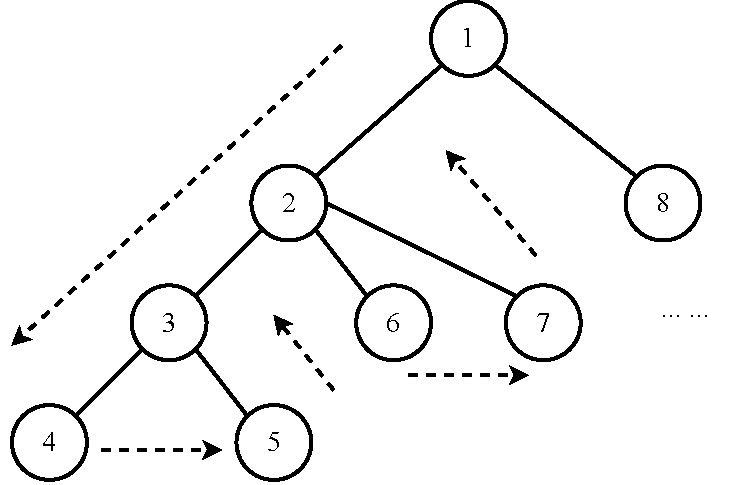
\includegraphics[scale=0.5]{img/dfs-tree-order}
 \caption{DFS search order.}
 \label{fig:dfs-tree}
\end{figure}

We call it deep first search (DFS), and widely use it in practice. Some programming environments, like Prolog, use DFS as the default evaluation model. Prolog define a maze with rules:

\lstset{language=Prolog}
\begin{lstlisting}
c(a, b). c(a, e).
c(b, c). c(b, f).
c(e, d), c(e, f).
c(f, c).
c(g, d). c(g, h).
c(h, f).
\end{lstlisting}

Where predicate $c(X, Y)$ means $X$ is connected with $Y$. This is a directed predicate, we can add a symmetric rule $c(Y, X)$ or create a undirected predicate. \Cref{fig:directed-graph} shows a directed graph. Given two places $X$ and $Y$, Prolog tells if they are connected with the following program:

\begin{figure}[htbp]
 \centering
 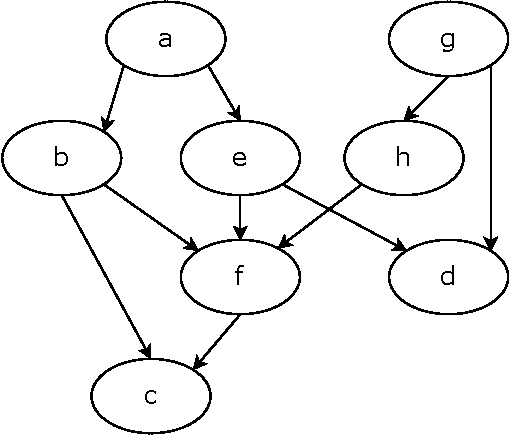
\includegraphics[scale=0.6]{img/directed-graph}
 \caption{A directed graph.}
 \label{fig:directed-graph}
\end{figure}

\lstset{language=Prolog}
\begin{lstlisting}
go(X, X).
go(X, Y) :- c(X, Z), go(Z, Y)
\end{lstlisting}

This program says: a place $X$ is connected with itself. Given two places $X$ and $Y$, if $X$ is connected with $Z$, and $Z$ is connected with $Y$, then $X$ is connected with $Y$. For multiple choices of $Z$, Prolog chooses one, and go on searching. It only tries another $Z$ if the recursive search fails and backtrack. This is exactly the DFS. We can apply DFS when only need a solution, but don't care the number of steps. For example, we need a way out of the maze, although it may not be the shortest.

\begin{Exercise}\label{ex:leap-frog}
\Question{Extend the pegs puzzle solution for $n$ pegs on each side.}
\end{Exercise}

\begin{Answer}[ref = {ex:leap-frog}]
\Question{Extend the pegs puzzle solution for $n$ pegs on each side.

We use $n$ to build the start/end states:
\begin{Haskell}
solve n = dfs [[start]] [] where
    dfs [] s = s
    dfs (c:cs) s
        | head c == end = dfs cs (reverse c:s)
        | otherwise = dfs ((map (:c) $ moves $ head c) ++ cs) s
    start = replicate n (-1) ++ [0] ++ replicate n 1
    end = reverse start
\end{Haskell}
}
\end{Answer}

\subsubsection{The wolf, goat, and cabbage puzzle}
\index{The wolf, goat, and cabbage puzzle}

This traditional puzzle says that a farmer need cross the river with a wolf, a goat, and a bucket of cabbage. There is a boat. Only the farmer can drive it. The boat can only carry one thing a time. The wolf would kill the goat; the goat would bite the cabbage if they stay alone without the farmer. The puzzle asks to find the best solution to cross the river.

Since the wolf doesn't bite the cabbage, the farmer can safely carry the goal to the other side and go back. No matter carry the wolf or the cabbage next, the farmer need carry one back to avoid conflict. To find the best the solution, we parallel try all options and compare. Despite the direction, count back and forth 2 steps. We check all possible status after 1 step, 2 steps, 3 steps, ... till the farmer and all things move to the other side at $n$ steps. This is the best solution.

But how to parallel try all options? Consider a lucky draw. People pick one from a box of colored balls. There is a black ball, and the rest are white. The one pick the black wins, or need return the white ball back to the box and wait for the next draw. We can define the rule that nobody try a second draw before all others pick. We line people in a queue. Every time the first person picks a ball, move to the tail if doesn't win. The queue ensures the fairness.

\begin{figure}[htbp]
 \centering
 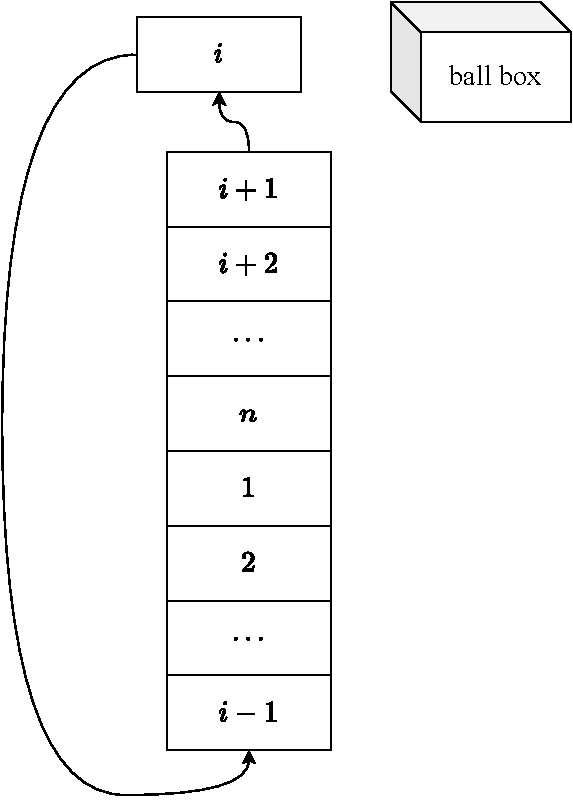
\includegraphics[scale=0.5]{img/luckydraw-queue}
 \caption{The $i$-th person de-queues, draw, then in-queue if doesn't win.}
 \label{fig:luck-draw}
\end{figure}

We apply the same method for the cross river puzzle. Let set $A$, $B$ contains the things on each side. When start, $A = \{w, g, c, p\}$ includes the wolf, the goat, the cabbage, and the farmer; $B=\nil$. We move the farmer with or without another element between $A$ and $B$. If a set doesn't contain the farmer, then it should has conflict elements. The goal is to swap elements in $A$ and $B$ with the fewest steps. We initiate a queue $Q$ with the start status: $A = \{w, g, c, p\}$, $B=\ni$. As far as $Q$ isn't empty, we de-queue the head, try all options, then en-queue the new status back to the tail. We find the solution when the head becomes $A=\nil$, $B=\{w, g, c, p\}$. \Cref{fig:bfs-tree} shows the search order. As all options at the same level are tried, we needn't backtrack.

\begin{figure}[htbp]
 \centering
 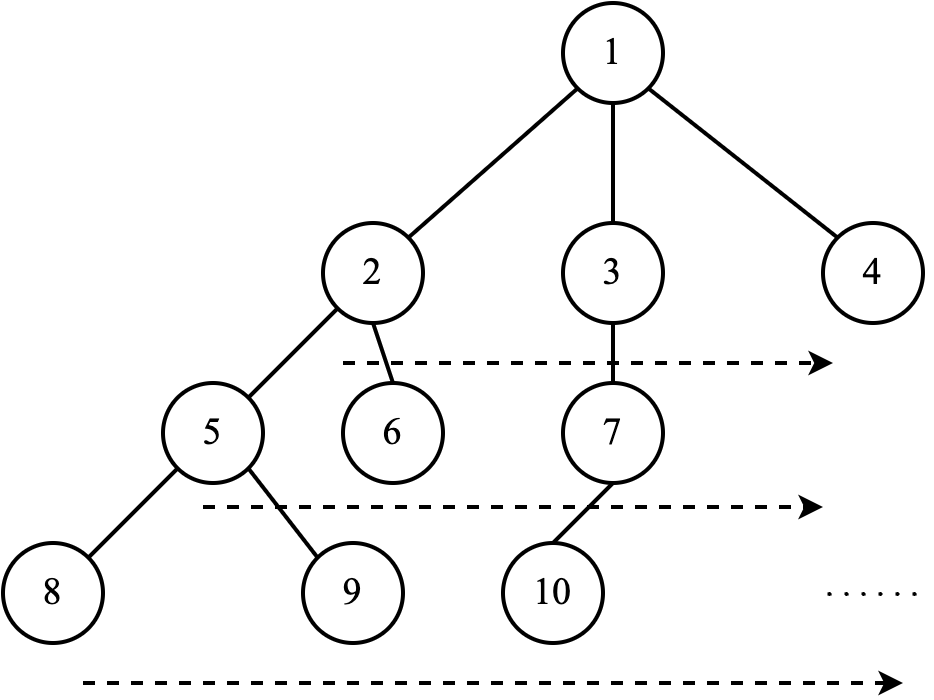
\includegraphics[scale=0.5]{img/bfs-tree-order}
 \caption{Start from 1, check all options 2, 3, 4 for the next step; then all option for the 3rd step, ...}
 \label{fig:bfs-tree}
\end{figure}

We can represent the set with a four bits binary number, each bit stands for an element, e.g., the wolf $w=1$, the goat $g=2$, the cabbage
$c=4$, and the farmer $p=8$. 0 is the empty set, 15 is the full set. 3 = 1 + 2, means the set \{wolf, goat\}. It's invalid because the wolf will kill the goat; 6 = 2 + 4, is another conflict \{goat, cabbage\}. Every time, we move the highest bit (8), with or without another bit (4, 2, 1) from one number to the other. The options are:

\be
mv\ A\ B = \begin{cases}
  B < 8: & [(A - 8 - i, B + 8 + i) | i \gets [0, 1, 2, 4], i = 0\ \text{or}\ A \overline{\land} i \neq 0]\\
  \text{otherwise}: & [(A + 8 + i, B - 8 - i) | i \gets [0, 1, 2, 4], i = 0\ \text{or}\ B \overline{\land} i \neq 0]
  \end{cases}
\ee

Where $\overline{\land}$ is bitwise-and. We start searching from $Q = \{[(15, 0)]\}$, as: $solve\ Q$

\be
\begin{array}{rcl}
solve\ \nil & = & \nil \\
solve\ Q & = & \begin{cases}
  A = 0: & reverse\ c, \text{where}: (A, B) = c, (c, Q') = pop\ Q \\
  \text{where}: & solve\ (pushAll\ (map\ (:c)\ (filter\ (valid\ c)\ (mv\ A\ B)))\ Q')
  \end{cases}
\end{array}
\ee

Where $valid\ c$ checks if the move $(A, B)$ is valid, neither is 3 or 6, and is new (not in $c$):

\be
A, B \neq 3\ \text{or}\ 6, (A, B) \notin c
\ee

Below is the iterative implementation:

\begin{algorithmic}[1]
\Function{Solve}{}
  \State $S \gets []$
  \State $Q \gets \{[(15, 0)]\}$
  \While{$Q \neq \nil$}
    \State $C \gets $ \Call{DeQ}{$Q$}
    \If{$C[1] = (0, 15)$}
      \State \textproc{Add}($S$, \Call{Reverse}{$C$})
    \Else
      \For{each $m$ in \Call{Moves}{$C$}}
        \If{\Call{Valid}{$m, C$}}
          \State \Call{EnQ}{$Q, m \cons C$}
        \EndIf
      \EndFor
    \EndIf
  \EndWhile
  \State \Return $S$
\EndFunction
\end{algorithmic}

It outputs two best solutions:

\btab{l|c|l}
Left & river & Right \\
\hline
wolf, goat, cabbage, farmer &   & \\
wolf, cabbage &   & goat, farmer \\
wolf, cabbage, farmer &   & goat \\
cabbage &   & wolf, goat, farmer \\
goat, cabbage, farmer &   & wolf \\
goat &   & wolf, cabbage, farmer \\
goat, farmer &   & wolf, cabbage \\
 &  & wolf, goat, cabbage, farmer
\etab

\btab{l|c|l}
Left & river & Right \\
\hline
 wolf, goat, cabbage, farmer & & \\
 wolf, cabbage & & goat, farmer \\
 wolf, cabbage, farmer & & goat \\
 wolf & & goat, cabbage, farmer \\
 wolf, goat, farmer & & cabbage \\
 goat & & wolf, cabbage, farmer \\
 goat, farmer & & wolf, cabbage \\
 & & wolf, goat, cabbage, farmer
\etab

\subsubsection{Water jugs puzzle}
\index{Water jugs puzzle}

Given two water jugs, 9 litres and 4 litres. How to get 6 litres from river? This puzzle has history back to ancient Greece. A story said the French mathematician Sim\`{e}on Denis Poisson solved this puzzle when he was a child. It also appears in Hollywood movie `Die-Hard 3'. P\`{o}lya uses this puzzle as an example of backwards induction\cite{how-to-solve-it}.

\begin{figure}[htbp]
 \centering
 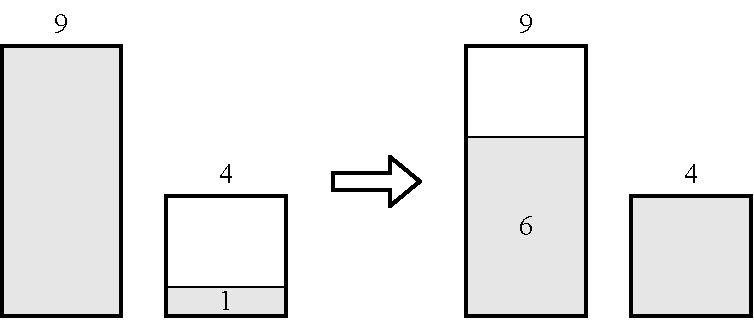
\includegraphics[scale=0.5]{img/jugs-last}
 \caption{The last two steps.}
 \label{fig:jugs-r1}
\end{figure}

After fill the 9 litres jug, then pour to the 4 litres jug twice, then we obtain 1 litre of water, as shown in \cref{fig:jugs-r2}. Backwards induction is a strategy, but not detailed algorithm. It can't directly answer how to get 2 litres of water from two jugs of 899 litres and 1147 litres for example.

\begin{figure}[htbp]
 \centering
 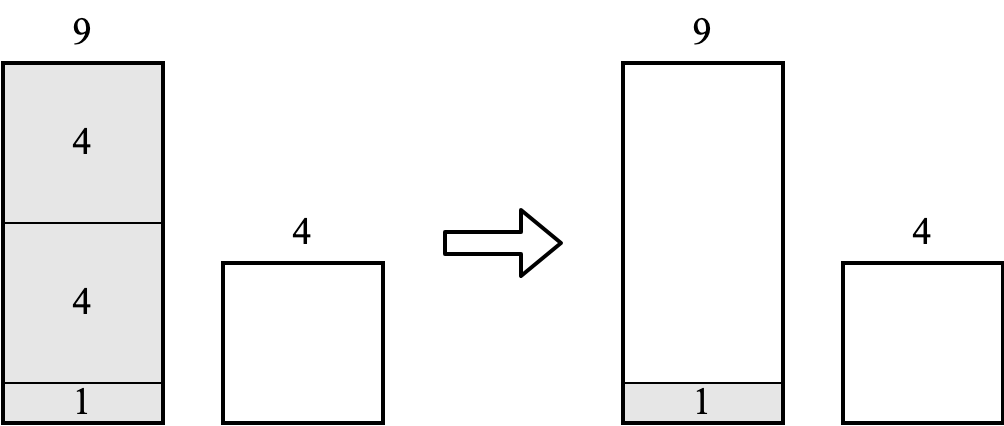
\includegraphics[scale=0.5]{img/jugs-last-two}
 \caption{Fill the bigger jug, then pour to the smaller one twice.}
 \label{fig:jugs-r2}
\end{figure}

Let the small jug be $A$, the big jug be $B$. There are 6 operations each time: (1) Fill jug $A$; (2) Fill jug $B$; (3) Empty jug $A$; (4) Empty jug $B$; (5) Pour from jug $A$ to $B$; (6) Pour water from jug $B$ to $A$. Below lists a series of operations (assume $a < b < 2a$).

\btab{l|l|l}
$A$ & $B$ & operation \\
\hline
0 & 0 & start \\
a & 0 & fill $A$ \\
0 & a & pour $A$ to $B$ \\
a & a & fill $A$ \\
2a - b & b & pour $A$ to $B$ \\
2a - b & 0 & empty $B$ \\
0 & 2a - b & pour $A$ to $B$ \\
a & 2a - b & fill $A$ \\
3a - 2b & b & pour $A$ to $B$ \\
... & ... & ... \\
\etab

Whatever operations, the water in each jug must be $xa + yb$, from some integers $x$ and $y$, where $a$ and $b$ are jug volumes. From the number theory, we can get $g$ litres of water if and only if $g$ is dividable by the greatest common divisor of $a$ and $b$, i.e., $gcd(a, b) | g$. If $gcd(a, b) = 1$ ($a$ and $b$ are coprime), then we can get any nature number $g$ litres of water. Although we know the existence of the solution, we don't know the detailed steps. We can solve the Diophantine equation $g = xa + yb$, design the operations from $x$ and $y$. Assume $x > 0, y < 0$, we fill jug $A$ total $x$ times, empty jug $B$ total $y$ times. For example, the small jug $a=3$ litres, the big jug $b=5$ litres, and the goal is to get $g=4$ litres of water. Because $4 = 3 \times 3 - 5$, we design below operations:

\btab{l|l|l}
$A$ & $B$ & operation \\
\hline
0 & 0 & start \\
3 & 0 & fill $A$ \\
0 & 3 & pour $A$ to $B$ \\
3 & 3 & fill $A$ \\
1 & 5 & pour $A$ to $B$ \\
1 & 0 & empty $B$ \\
0 & 1 & pour $A$ to $B$ \\
3 & 1 & fill $A$ \\
0 & 4 & pour $A$ to $B$ \\
\etab

We fill jug $A$ 3 times, empty jug $B$ 1 time. We can apply the {\em Extended Euclid algorithm} in number theory to find $x$ and $y$:

\be
(d, x, y) = gcd_{ext}(a, b)
\ee

Where $d = gcd(a, b)$, $ax + by = d$. Assume $a < b$, the quotient $q$ and remainder $r$ satisfy $b = a q + r$. The common divisor $d$ divides both $a$ and $b$, hence $d$ divides $r$ too. Because $r < a$, we can scale down the problem to find $gcd(a, r)$:

\be
(d, x', y') = gcd_{ext}(r, a)
\label{eq:recursive-ext-gcd}
\ee

Where $d = x' r + y' a$. Substitute $r = b - a q$ in:

\be
\begin{array}{rcl}
d & = & x' (b - a q) + y' a \\
  & = & (y' - x' q) a + x' b
\end{array}
\ee

Compare with $d = ax + by$, we have the following recursion:

\be
\begin{cases}
  x & = y' - x' \dfrac{b}{a} \\
  y & = x'
\end{cases}
\ee

The edge case happens when $a=0$: $gcd(0, b) = b = 0 a + 1 b$. Hence the extended Euclid algorithm can be defined as:

\be
\begin{array}{rcl}
gcd_{ext}(0, b) & = & (b, 0, 1) \\
gcd_{ext}(a, b) & = & (d, y' - x' \dfrac{b}{a}, x')
\end{array}
\ee

Where $d$, $x'$, $y'$ are defined in \cref{eq:recursive-ext-gcd}. If $g = md$, then $mx$ and $my$ is a solution; if $x < 0$, for example: $gcd_{ext}(4, 9) = (1, -2, 1)$. Since $d = x a + y b$, we repeatedly add $x$ by $b$, and decrease $y$ by $a$ till $x > 0$. Such solution may not be the best one. For example, to get 4 litres of water from two jugs of 3 and 5 liters, the extended Euclid algorithm gives 23 steps:

\begin{Verbatim}[fontsize=\footnotesize]
[(0,0),(3,0),(0,3),(3,3),(1,5),(1,0),(0,1),(3,1),
(0,4),(3,4),(2,5),(2,0),(0,2),(3,2),(0,5),(3,5),
(3,0),(0,3),(3,3),(1,5),(1,0),(0,1),(3,1),(0,4)]
\end{Verbatim}

While the best solution only need 6 steps:

\begin{Verbatim}[fontsize=\footnotesize]
[(0,0),(0,5),(3,2),(0,2),(2,0),(2,5),(3,4)]
\end{Verbatim}

There are infinite many solutions for the Diophantine equation $g = x a + b y$. The smaller $|x| + |y|$, the fewer steps. We can apply the same method as the `cross river' puzzle. Try the 6 operations (fill $A$, fill $B$, pour $A$ into $B$, pour $B$ into $A$, empty $A$ and
empty $B$) in parallel to find the best solution. We use a queue to arrange the attempts. The element in the queue are series of pairs $(p, q)$, where $p$ and $q$ are waters in each jug, as operations from the beginning. The queue starts from $\{[(0, 0)]\}$.

\be
solve\ a\ b\ g = bfs \{ [(0, 0)] \}
\ee

As far as the queue isn't empty, we pop a sequence from the head. If the last pair of the sequence contains $g$ litres, we find a solution. We reverse and output the sequence; otherwise, we try 6 operations atop the latest pair, filter out the duplicated ones and add back to the queue.

\be
\begin{array}{rcl}
bfs\ \nil & = & [\ ] \\
bfs\ Q & = & \begin{cases}
  p\ \text{or}\ q = g: & \textit{reverse}\ s, \text{where}: (p, q) = head\ s, (s, Q') = pop\ Q \\
  \text{otherwise}: & bfs\ (pushAll\ (map\ (:s)\ (try\ s))\ Q')
    \end{cases}
\end{array}
\ee

\be
try\ s = filter\ (\notin s)\ [f\ (p, q) | f \gets \{fl_A, fl_B, pr_A, pr_B, em_A, em_B\}]
\ee

Where:

\be
\begin{cases}
fl_A\ (p, q) = (a, q) \\
fl_B\ (p, q) = (p, b) \\
em_A\ (p, q) = (0, q) \\
em_B\ (p, q) = (p, 0) \\
pr_A\ (p, q) = (\max(0, p + q - b), \min(x + y, b)) \\
pr_B\ (p, q) = (\min(x + y, a), \max(0, x + y - a)) \\
\end{cases}
\ee

This method returns the solution with the fewest steps. To avoid storing the complete operation sequence in the queue, we can use a global history list, and link every operation back to its predecessor. As shown in \cref{fig:water-jugs}, the start state is (0, 0), only `fill A' and `fill B' are applicable. We next try `fill B' atop (3, 0), record the new state (3, 5). If apply `empty A' to (3, 0), we'll go back to the starting point (0, 0). We skip it (shaded state). We add a `parent' reference to each node in \cref{fig:water-jugs}, and backtrack along it to the beginning.

\begin{figure}[htbp]
  \centering
  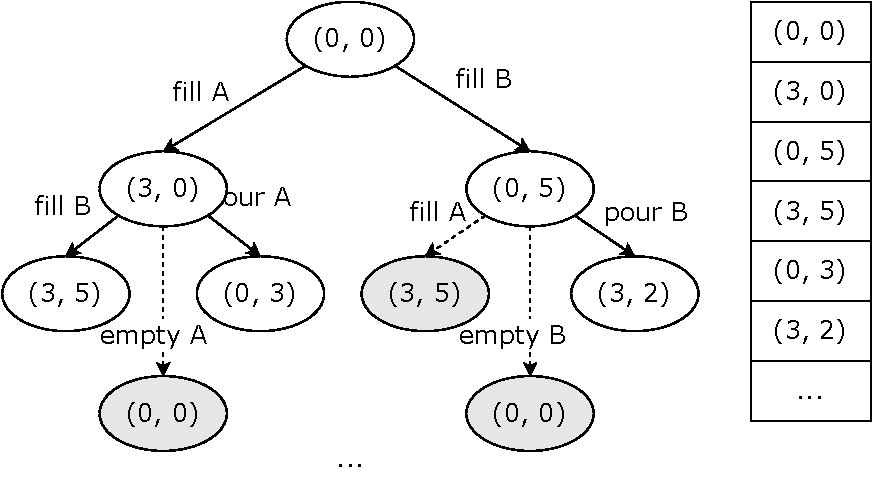
\includegraphics[scale=0.5]{img/water-jugs}
  \caption{Store all states with a global list.}
  \label{fig:water-jugs}
\end{figure}

\begin{algorithmic}[1]
\Function{Solve}{$a, b, g$}
  \State $Q \gets \{(0, 0, \text{NIL})\}$  \Comment{Queue}
  \State $V \gets \{(0, 0, \text{NIL})\}$  \Comment{Visited set}
  \While{$Q \neq \nil$}
    \State $s \gets$ \Call{Pop}{$Q$}
    \If{$p(s) = g$ or $q(s) = g$}
      \State \Return \Call{Back-track}{$s$}
    \Else
      \For{each $c$ in \Call{Expand}{$s, a, b$}}
        \If{$c \neq s$ and $c \notin V$}
          \State \Call{Push}{$Q, c$}
          \State \Call{Add}{$V, c$}
        \EndIf
      \EndFor
    \EndIf
  \EndWhile
  \State \Return NIL
\EndFunction
\Statex
\Function{Expand}{$s, a, b$}
  \State $p \gets p(s), q \gets q(s)$
  \State \Return $[(a, q, s), (p, b, s), (0, q, s), (p, 0, s), (\max(0, p + q - b), \min(p + q, b), s), (\min(p + q, a), \max(0, p + q - a), s)]$
\EndFunction
\Statex
\Function{Back-track}{$s$}
  \State $r \gets [\ ]$
  \While{$s \neq$ NIL}
    \State $(p, q, s') = s$
    \State $r \gets (p, q) \cons r$
    \State $s \gets s'$
  \EndWhile
  \State \Return $r$
\EndFunction
\end{algorithmic}

\begin{Exercise}\label{ex:water-jugs-puzzle}
\Question{Improve the extended Euclid algorithm, find the $x$ and $y$ that minimize $|x| + |y|$ for the optimal solution for the two jugs puzzle.}
\end{Exercise}

\begin{Answer}[ref = {ex:water-jugs-puzzle}]
\Question{Improve the extended Euclid algorithm, find the $x$ and $y$ that minimize $|x| + |y|$ for the optimal solution for the two jugs puzzle.

\begin{Haskell}
import Data.List
import Data.Function (on)

-- Extended Euclidean Algorithm
gcmex a 0 = (a, 1, 0)
gcmex a b = (g, y', x' - y' * (a `div` b)) where
  (g, x', y') = gcmex b (a `mod` b)

-- Solve the linear Diophantine equation ax + by = c
solve a b c | c `mod` g /= 0 = (0, 0, 0, 0) -- no solution
            | otherwise = (x1, u, y1, v)
  where
    (g, x0, y0) = gcmex a b
    (x1, y1) = (x0 * c `div` g, y0 * c `div` g)
    (u, v) = (b `div` g, a `div` g)

-- Minimize |x| + |y|
jars a b c = (x, y) where
  (x1, u, y1, v) = solve a b c
  x = x1 - k * u
  y = y1 + k * v
  k = minimumBy (compare `on` (\i -> abs (x1 - i * u) +
                                     abs (y1 + i * v))) [-m..m]
  m = max (abs x1 `div` u) (abs y1 `div` v)

-- Populate the steps
water a b c = if x > 0 then pour a x b y
              else map swap $ pour b y a x
  where
    (x, y) = jars a b c

-- Pour from a to b, fill a for x times, and empty b for y times.
pour a x b y = steps x y [(0, 0)]
  where
    steps 0 0 ps = reverse ps
    steps x y ps@((a', b'):_)
      | a' == 0 = steps (x - 1) y ((a, b'):ps)  -- fill a
      | b' == b = steps x (y + 1) ((a', 0):ps)  -- empty b
      | otherwise = steps x y ((max (a' + b' - b) 0,
                                min (a' + b') b):ps) -- a to b
\end{Haskell}

See section 2.2.3, chapter 2 in `isomorphism - mathematics of programming' for more details.
}
\end{Answer}

\subsubsection{Kloski}
\index{Kloski puzzle}

Kloski is a block slide puzzle, as shown in \cref{fig:klotski-cn}. There are 10 blocks of 3 sizes: 4 pieces of $1 \times 1$; 4 pieces of $1 \times 2$, 1 piece of $2 \times 1$, 1 piece of $2 \times 2$. The goal is to slide the big block to the bottom slot. \Cref{fig:klotski-jp} shows variants of this puzzle in Japan.

\begin{figure}[htbp]
 \centering
 \subcaptionbox{Initial layout}{\includegraphics[scale=0.5]{img/klotski-cn1}} \hspace{.01\textwidth}
 \subcaptionbox{Layout after several movements}{\includegraphics[scale=0.5]{img/klotski-cn2}}
 \caption{`Huarong Escape', the traditional Chinese Kloski puzzle.}
 \label{fig:klotski-cn}
\end{figure}

\begin{figure}[htbp]
 \centering
 \includegraphics[scale=0.5]{img/klotski-jp}
 \caption{`Daughter in the box', the Japanese Kloski puzzle.}
 \label{fig:klotski-jp}
\end{figure}

We define the board as a $5 \times 4$ matrix, the row and column start from 0. Label the pieces from 1 to 10. 0 means empty cell. The matrix $M$ gives the initial layout. The cells with value $i$ is occupied by piece $i$. We use a map $L$ to represent the layout, where $L[i]$ is the set of cells occupied by piece $i$. For example, $L[4] = \{(2, 1), (2, 2)\}$ means the 4th piece occupies cells $(2, 1)$ and $(2, 2)$. Label all 20 cells from 0 to 19, we can convert a pair of row, col to label: $c = 4y + x$. The 4th piece occupies cells $L[4] = \{9, 10\}$.

\[
\begin{array}{cc}
M = \left [
  \begin{array}{cccc}
  1 & 10 & 10 & 2 \\
  1 & 10 & 10 & 2 \\
  3 & 4 & 4 & 5 \\
  3 & 7 & 8 & 5 \\
  6 & 0 & 0 & 9
  \end{array}
\right ] &
L = \left \{
  \begin{array}{l}
  1 \mapsto \{0, 4\}, 2 \mapsto \{3, 7\}, 3 \mapsto \{8, 12\}, \\
  4 \mapsto \{9, 10\}, 5 \mapsto \{11, 15\}, \\
  6 \mapsto \{16\}, 7 \mapsto \{ 13 \}, 8 \mapsto \{ 14 \}, \\
  9 \mapsto \{ 19 \}, 10 \mapsto \{1, 2, 5, 6\}
  \end{array}
\right \}
\end{array}
\]

Define map $\varphi(M) \mapsto L$ and its reverse $\varphi^{-1}(L) \mapsto M$ to convert board and layout:

\begin{algorithmic}[1]
\Function{$\varphi$}{$M$}
  \State $L \gets \{ \}$
  \For{$y \gets 0 \sim 4$}
    \For{$x \gets 0 \sim 3$}
      \State $k \gets M[y][x]$
      \State $L[k] \gets$ \Call{Add}{$L[k], 4y + x$}
    \EndFor
  \EndFor
  \State \Return $L$
\EndFunction
\Statex
\Function{$\varphi^{-1}$}{$L$}
  \State $M \gets [[0] \times 4] \times 5$
  \For{each $(k \mapsto S)$ in $L$}
    \For{each $c$ in $S$}
      \State $x \gets c \bmod 4, y \gets \lfloor c / 4\rfloor$
      \State $M[y][x] \gets k$
    \EndFor
  \EndFor
  \State \Return $M$
\EndFunction
\end{algorithmic}

We try all the 10 blocks in 4 directions: up, down, left, and right. For board matrix, the movement means: $(\Delta y, \Delta x) = (0, \pm 1), (\pm 1, 0)$; for layout of cell labels, it means: $d = \pm 1, \pm 4$. For example, move piece $L[i] = \{c_1, c_2\}$ to left, it becomes: $\{c_1 -1, c_2 -1\}$. We need avoid invalid movement in two edge cases: $d = 1, c \bmod 4 = 3$ and $d = -1, c \bmod 4 = 0$, they are invalid because the piece jump from one side to the other. Consider the two free cells, there are at most 8 movements. For example, the first step only have 4 options: move piece 6 right, move piece 7 or 8 down, move piece 9 left. \Cref{fig:klotski-valid-move} shows how to verify the movement is valid.

\begin{figure}[htbp]
 \centering
 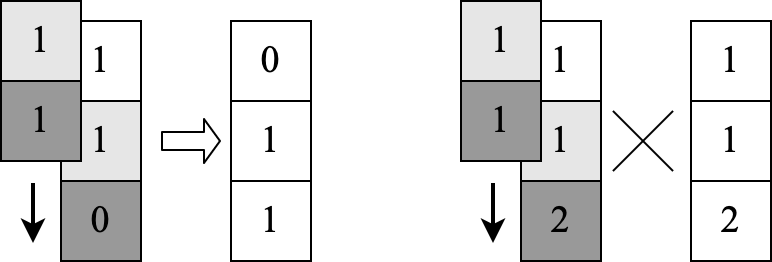
\includegraphics[scale=0.7]{img/klotski-valid-mv}
 \caption{Left: two cells of 1 can move; Right: the lower cell of 1 conflicts with the cell of 2.}
 \label{fig:klotski-valid-move}
\end{figure}

For the movement of piece $k$, it is valid if the target cells have value of 0 or $k$:

\be
\begin{array}{rl}
valid\ L[k]\ d: & \\
\forall c \in L[k] \Rightarrow & y = \lfloor c / 4 \rfloor + \lfloor d / 4 \rfloor, x = (c \bmod 4) + (d \bmod 4), \\
& (0, 0) \leq (y, x) \leq (4, 3), M[y][x] \in \{k, 0\}
\end{array}
\ee

We may return to some layout after a series of slides. It's insufficient to only avoid duplicated matrix. Although $M_1 \neq M_2$, they are essentially the same layout.

\[
\begin{array}{cc}
M_1 = \left [
  \begin{array}{cccc}
  1 & 10 & 10 & 2 \\
  1 & 10 & 10 & 2 \\
  3 & 4 & 4 & 5 \\
  3 & 7 & 8 & 5 \\
  6 & 0 & 0 & 9
  \end{array}
\right ] &
M_2 = \left [
  \begin{array}{cccc}
  2 & 10 & 10 & 1 \\
  2 & 10 & 10 & 1 \\
  3 & 4 & 4 & 5 \\
  3 & 7 & 6 & 5 \\
  8 & 0 & 0 & 9
  \end{array}
\right ]
\end{array}
\]

We need avoid duplicated layout. Treat all pieces of the same size same, we define normalized layout as: $\|L\| = \{ p | (k \mapsto p) \in L\}$, the set of all cell labels in $L$. Both matrix above have the same normalized layout as \{\{1, 2, 5, 6\}, \{0, 4\}, \{3, 7\}, \{8, 12\}, \{9, 10\}, \{11, 15\}, \{16\}, \{13\}, \{14\}, \{19\}\}. We also need avoid mirrored layout, for example:

\[
\begin{array}{cc}
M_1 = \left [
  \begin{array}{cccc}
  10 & 10 & 1 & 2 \\
  10 & 10 & 1 & 2 \\
  3 & 5 & 4 & 4 \\
  3 & 5 & 8 & 9 \\
  6 & 7 & 0 & 0
  \end{array}
\right ] &
M_2 = \left [
  \begin{array}{cccc}
  3 & 1 & 10 & 10 \\
  3 & 1 & 10 & 10 \\
  4 & 4 & 2 & 5 \\
  7 & 6 & 2 & 5 \\
  0 & 0 & 9 & 8
  \end{array}
\right ]
\end{array}
\]

Both have the same normalized layout. Define the mirror function:

\be
mirror(\|L\|) = \{\{ f(c) | c \in s \} | s \in \|L\|\}
\ee

Where $f(c) = 4y' + x', y' = \lfloor c / 4 \rfloor, x' = 3 - (c \bmod 4)$. We use a queue to arrange the search. The element in the queue has two parts: a series of movements, and the resulted layout. The movement is a pair $(k, d)$, means move piece $k$ by $d$ ($\pm 1, \pm 4$). Initialize the queue $Q = \{(s, [\ ])\}$, where $s$ is the start layout. As far as the queue isn't empty $Q \neq \nil$, we get its head, examine whether the big block (piece 10) arrives at $t = \{13, 14, 17, 18\}$, i.e., $L[10] = t$. Terminates if yes; otherwise, we try up, down, left, right for every piece, add every valid $(k, d)$, that leads to unique layout to the queue. We use a set $H$ to records all visited normalized layouts to avoid repetition.

\be
\begin{array}{rcl}
solve\ \nil\ H\ & = & [\ ] \\
solve\ Q\ H\ & = & \begin{cases}
  L[10] = t: & \textit{reverse}\ ms, \text{where}: ((L, ms), Q') = pop\ Q \\
  \text{otherwise}: & solve\ (pushAll\ cs\ Q')\ H' \\
  \end{cases}
\end{array}
\ee

Where $cs = [(move\ L\ e, e \cons ms) | e \gets expand\ L]$ are the new movements expanded.

\be
\begin{array}{rl}
expand\ L = \{(k, d) | & k \gets [1, 2, ..., 10], d \gets [\pm 1, \pm 4], \\
  &  valid\ k\ d, unique\ k\ d \} \\
\end{array}
\ee

Function $move$ slides piece $L[k]$ by $d$ to: $move\ L\ (k, d) = map\ (+ d)\ L[k]$. $unique$ checks if the normalized layout $\|L'\| \notin H$ and its mirror $mirror(\|L'\|) \notin H$. Add them to $H'$ if new. Below are the iterative implementation. The solution has 116 steps (1 cell a step). The last 3 are:

\begin{algorithmic}[1]
\Function{Solve}{$s, e$}
  \State $H \gets \{\|s\|\}$
  \State $Q \gets \{(s, \nil)\}$
  \While{$Q \neq \nil$}
    \State $(L, p) \gets$ \Call{Pop}{$Q$}
    \If{$L[10] = e$}
      \State \Return $(L, p)$
    \Else
      \For{each $L'$ in \Call{Expand}{$L, H$}}
        \State \Call{Push}{$Q, (L', L)$}
        \State \Call{Add}{$H, \|L'\|$}
      \EndFor
    \EndIf
  \EndWhile
  \State \Return $\nil$
\EndFunction
\end{algorithmic}

\begin{Verbatim}[fontsize=\footnotesize]
['5', '3', '2', '1']
['5', '3', '2', '1']
['7', '9', '4', '4']
['A', 'A', '6', '0']
['A', 'A', '0', '8']

['5', '3', '2', '1']
['5', '3', '2', '1']
['7', '9', '4', '4']
['A', 'A', '0', '6']
['A', 'A', '0', '8']

['5', '3', '2', '1']
['5', '3', '2', '1']
['7', '9', '4', '4']
['0', 'A', 'A', '6']
['0', 'A', 'A', '8']
\end{Verbatim}

\index{BFS} \index{Breadth-first search}
The cross river puzzle, water jugs puzzle, and the Kloski puzzle share the common solution structure. Similar to the DFS, they have start and end states. For example, the cross river puzzle starts with all things on one side, the other side is empty; it ends with all things on the other side. The water jugs puzzle starts with tow empty jugs; it ends with either jug has $g$ litres of water. The Klotski puzzle starts with some layout, it ends with some layout that the big block arrives at the bottom slot. Every puzzle have a set of rules, transfer from a state to another. We `parallel' try all options. We don't search further until complete trying all options of the same step. This search strategy ensure we find the solution with the fewest step before others. Because we expand horizontally, it's called Breadth-first search. \Cref{fig:dfs-bfs-tree} compares DFS and BFS.

\begin{figure}[htbp]
 \centering
 \subcaptionbox{DFS}{ 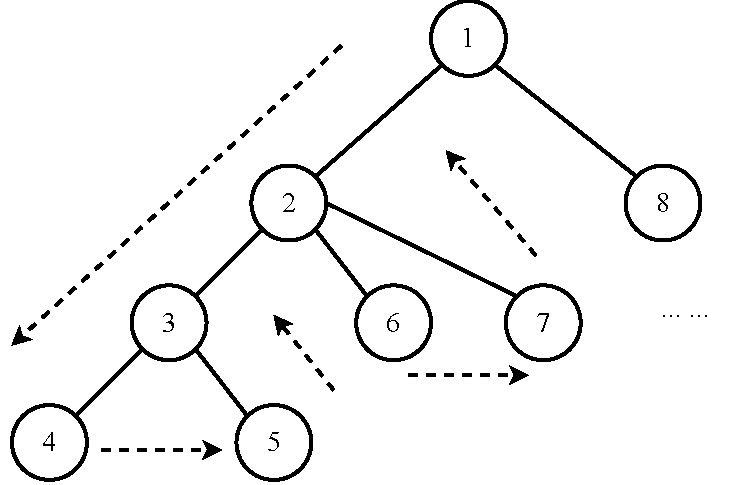
\includegraphics[scale=0.45]{img/dfs-tree-order}}
 \subcaptionbox{BFS}{ 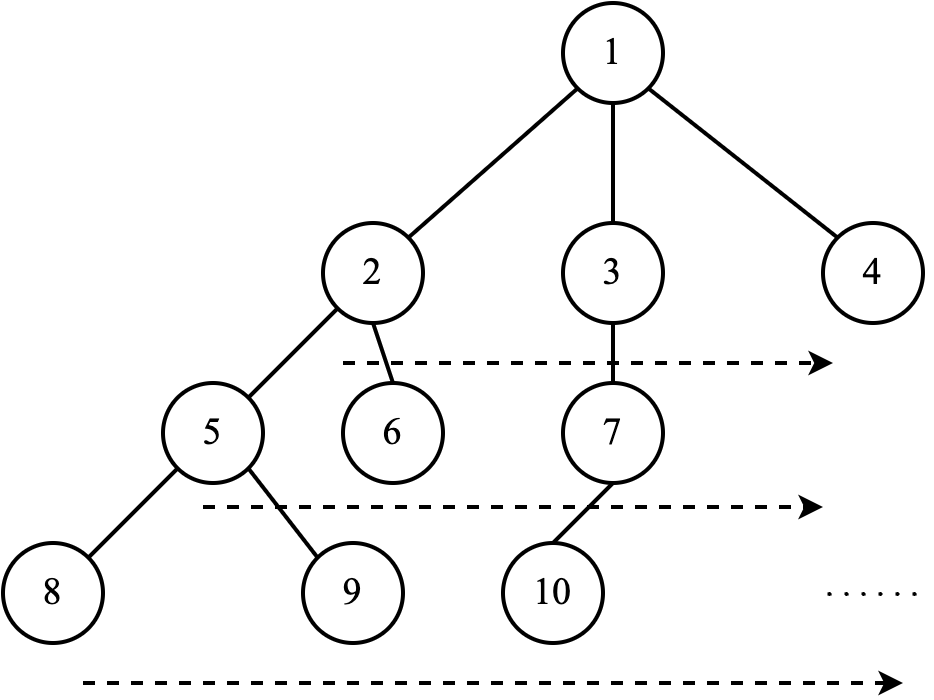
\includegraphics[scale=0.45]{img/bfs-tree-order}}
 \caption{DFS and BFS.}
 \label{fig:dfs-bfs-tree}
\end{figure}

Because we can't really search in parallel, we realize BFS with a queue. Repeat de-queue the candidate with fewer steps from head, and en-queue new candidate with more steps to tail. BFS provides a simple method to search the solution with the fewest steps. However, it can't directly search for generic optimal solution. Consider the directed graph in \cref{fig:weighted-dag}, the length of each section varies. We can't use BFS to find the shortest path between two cities. For example, the shortest path from $a$ to $c$ is not the one with the fewest steps: $a \to b \to c$. The total length is 22, but the path with more steps $a \to e \to f \to c$ has the length of 20.

\begin{figure}[htbp]
 \centering
 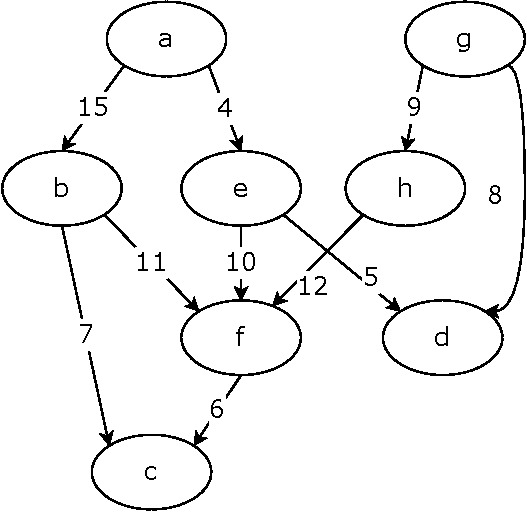
\includegraphics[scale=0.5]{img/weighted-dag}
 \caption{A weighted directed graph.}
 \label{fig:weighted-dag}
\end{figure}

\begin{Exercise}\label{ex:conway-slide-puzzle}
\Question{John Conway\footnote{John Conway (1937 - 2020), British mathematician.} gives a slide tile puzzle. \Cref{fig:conway7} is a simplified example. There are 8 cells, 7 are occupied. Label the pieces from 1 to 7. Each piece can slide to the connected free cell. (two cells are connected if there is a line between them.) How to reverse the pieces from 1, 2, 3, 4, 5, 6, 7 to 7, 6, 5, 4, 3, 2, 1 by sliding? Write a program to solve this puzzle.
\begin{center}
 \centering
 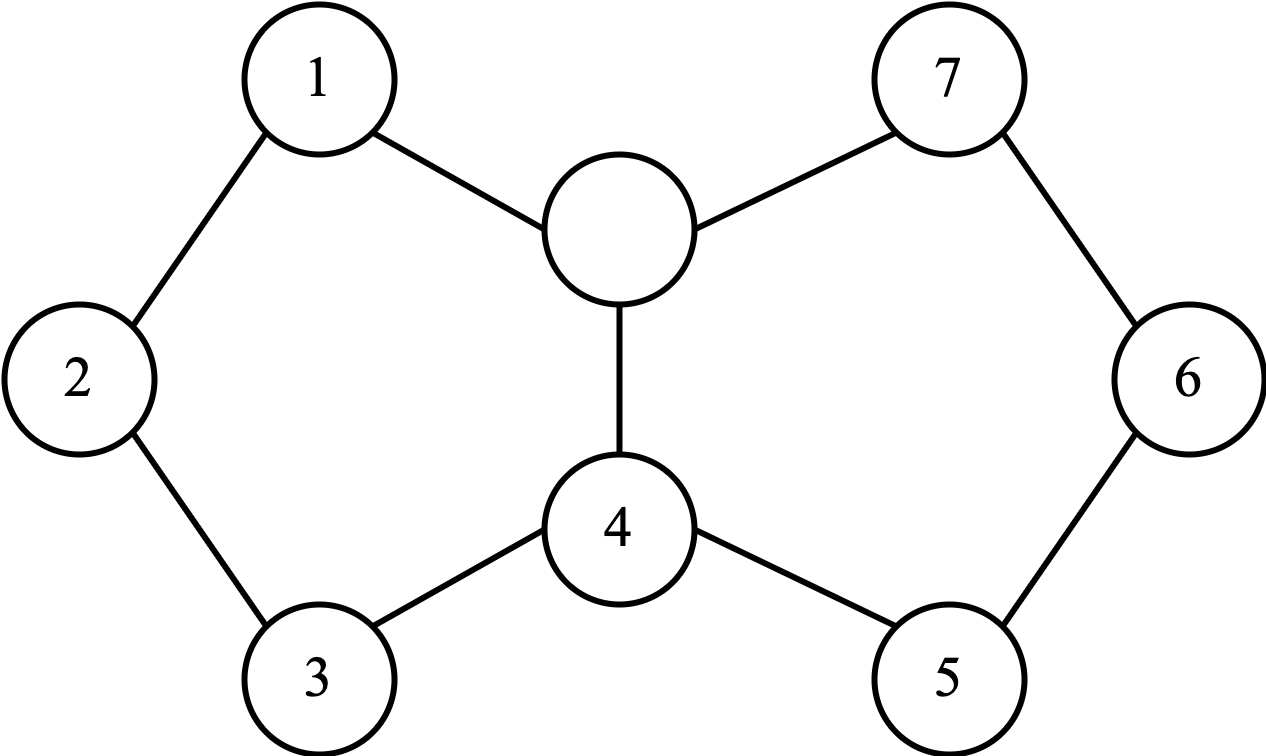
\includegraphics[scale=0.5]{img/conway-7-slide}
 %\input{img/conway7.tex}
 \captionof{figure}{Conway slide puzzle}
 \label{fig:conway7}
\end{center}
}
\end{Exercise}

\begin{Answer}[ref = {ex:conway-slide-puzzle}]
\Question{Conway slide puzzle.

We use 8 numbers from 0 to 7 to represents pieces, where 0 is the free cell. The pieces next to 0 can slide in, we represent it as the number 0 move forward/backward in a permutation. When move forward beyond tail, it goes back to the head; when move backward beyond head, it goes to the tail. Particularly, when 0 is the first, it can swap with the 5th piece and vice versa. The solution is very long with 12948 steps. The last several steps is as below.

\begin{Haskell}
start = [0..7]
end = 0:[7,6..1]

solve1 = dfs [[start]] where
  dfs [] = []
  dfs (c:cs)
    | head c == end = reverse c
    | otherwise = dfs ((map (:c) $ moves c) ++ cs)

moves (s:visited) = filter (`notElem` visited) [fwd s, bk s, cut s]
  where
    fwd xs = case break (0 ==) xs of
      (as, 0:b:bs) -> as ++ (b:0:bs)
      (a:as, [0]) -> 0:as ++ [a]
    bk xs = case break (0 ==) xs of
      ([], 0:bs) -> bs ++ [0]
      (as, 0:bs) -> (init as) ++ (0 : last as : bs)
    cut xs = case splitAt 4 xs of
      ((0:as), (x:bs)) -> (x:as) ++ (0:bs)
      ((x:as), (0:bs)) -> (0:as) ++ (x:bs)
      _ -> xs
\end{Haskell}

\begin{Verbatim}[fontsize=\footnotesize]
...
[1,0,7,6,5,4,3,2],[1,7,0,6,5,4,3,2],[1,7,6,0,5,4,3,2],[1,7,6,5,0,4,3,2],
[1,7,6,5,4,0,3,2],[1,7,6,5,4,3,0,2],[1,7,6,5,4,3,2,0],[0,7,6,5,4,3,2,1]
\end{Verbatim}
}
\end{Answer}

\subsection{Greedy algorithm}
\index{Greedy algorithm}

People need find the `best' solution to minimize time, space, cost, energy, and etc. It's not easy to find the optimal solution within limited resource. Many problem don't have solution in polynomial time, however, there exist simple solution for a small portion of special problems.

\subsubsection{Huffman coding}
\index{Huffman coding}
Huffman coding encodes information with the shortest length. The ASCII code needs 7 bits to encode characters, digits, and symbols. It can represent $2^7 = 128$ symbols. We need at least $\log_2 n$ 0/1 bits to distinguish $n$ symbols. Below table encodes upper case English letters, maps A to Z from 0 to 25, each with 5 bits. Zero is padded as 00000 but not 0. Such scheme is called fixed-length coding.

\btab{l|l||l|l}
char & code & char & code \\
\hline
A & 00000 & N & 01101 \\
B & 00001 & O & 01110 \\
C & 00010 & P & 01111 \\
D & 00011 & Q & 10000 \\
E & 00100 & R & 10001 \\
F & 00101 & S & 10010 \\
G & 00110 & T & 10011 \\
H & 00111 & U & 10100 \\
I & 01000 & V & 10101 \\
J & 01001 & W & 10110 \\
K & 01010 & X & 10111 \\
L & 01011 & Y & 11000 \\
M & 01100 & Z & 11001 \\
\hline
\etab

It encodes `INTERNATIONAL' to a binary number of 65 bits:

\begin{Verbatim}[fontsize=\footnotesize]
00010101101100100100100011011000000110010001001110101100000011010
\end{Verbatim}

Another scheme is variable-length coding. Encode A as single bit 0, encode C as 10 of two bits, encode Z as 11001 of 5 bits. Although the code length is shorter, it has ambiguity when decode. For example, the binary number 1101 can stand for 1 followed with 101 (decoded as `BF') or 110 followed with 1 (decoded as `GB'), or 1101 (decoded as N). The Morse code is variable-length. It encodes the most used letter `E' as `.', encodes `Z' as `- -..'. Particularly, it uses a special pause separator to indicate the termination of a code, eliminates the ambiguity. Below code table is ambiguity free:

\btab{l|l||l|l}
char & code & char & code \\
\hline
A & 110 & E & 1110 \\
I & 101 & L & 1111 \\
N & 01 & O & 000 \\
R & 001 & T & 100 \\
\hline
\etab

It encodes `INTERNATIONAL' with 38 bits only:

\begin{Verbatim}[fontsize=\footnotesize]
10101100111000101110100101000011101111
\end{Verbatim}

The reason why it's ambiguity free is because there is no code is the prefix of the other. Such code is called {\em prefix-code}. (but not the `non-prefix code'.) Since the prefix-code needn't separator, we can further shorten the code length. Given a text, can we find a prefix-code scheme, that produces the shortest code? In 1951, Robert M. Fano told the class that those who could solve this problem needn't take the final exam. Huffman was still a student in MIT\cite{Huffman}. He almost gave up and started preparing the final exam when found the answer. Huffman created the coding table according to the frequency of the symbol appeared in the text. The more used one is assigned with the shorter code. Process the text, and calculate the occurrence for each symbol. Define the weight as the frequency. Huffman uses a binary tree to generate the prefix-code. The symbols are stored in the leaf nodes. Traverse from the root to generate the code, add 0 when go left, 1 when go right, as shown in \cref{fig:huffman-tr}. For example, starting from the root, go left, then right, we arrive at `N'. Therefore, `N' is encoded as `01'; While the paths of `A' is right, right, left, encoded as `110'.

\begin{figure}[htbp]
 \centering
 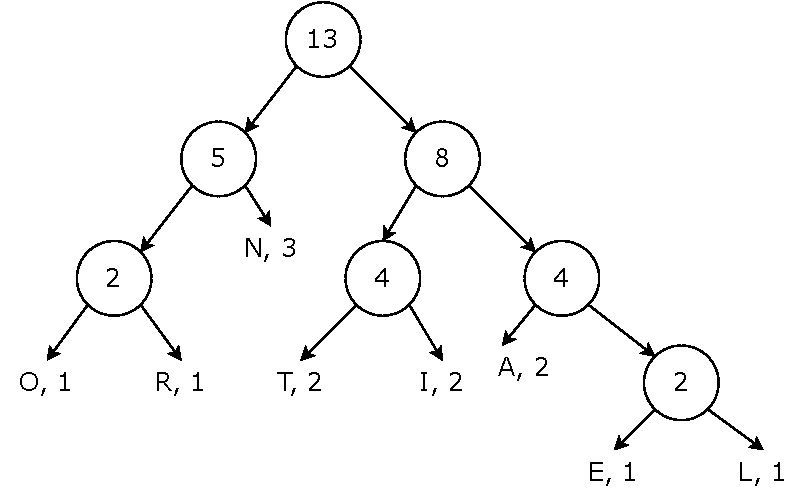
\includegraphics[scale=0.5]{img/huffman-tr}
 \caption{Huffman tree}
 \label{fig:huffman-tr}
\end{figure}

We can use the tree to decode as well. Scan the binary bits, go left for 0, and right for 1. When arrive at a leaf, we decode the symbol from it. Then restart from the root to continue scan. Huffman build the tree in bottom-up way. When start, wrap all symbols in leaves. Every time, pick two nodes with the minimum weights, merge them to a branch node of weight $w$. where $w = w_1 + w_2$ is the sum of the two weights. Repeat pick and merge the two smallest weighted trees till we get the final tree, as shown in \cref{fig:huffman-build}.

\begin{figure}[htbp]
  \centering
  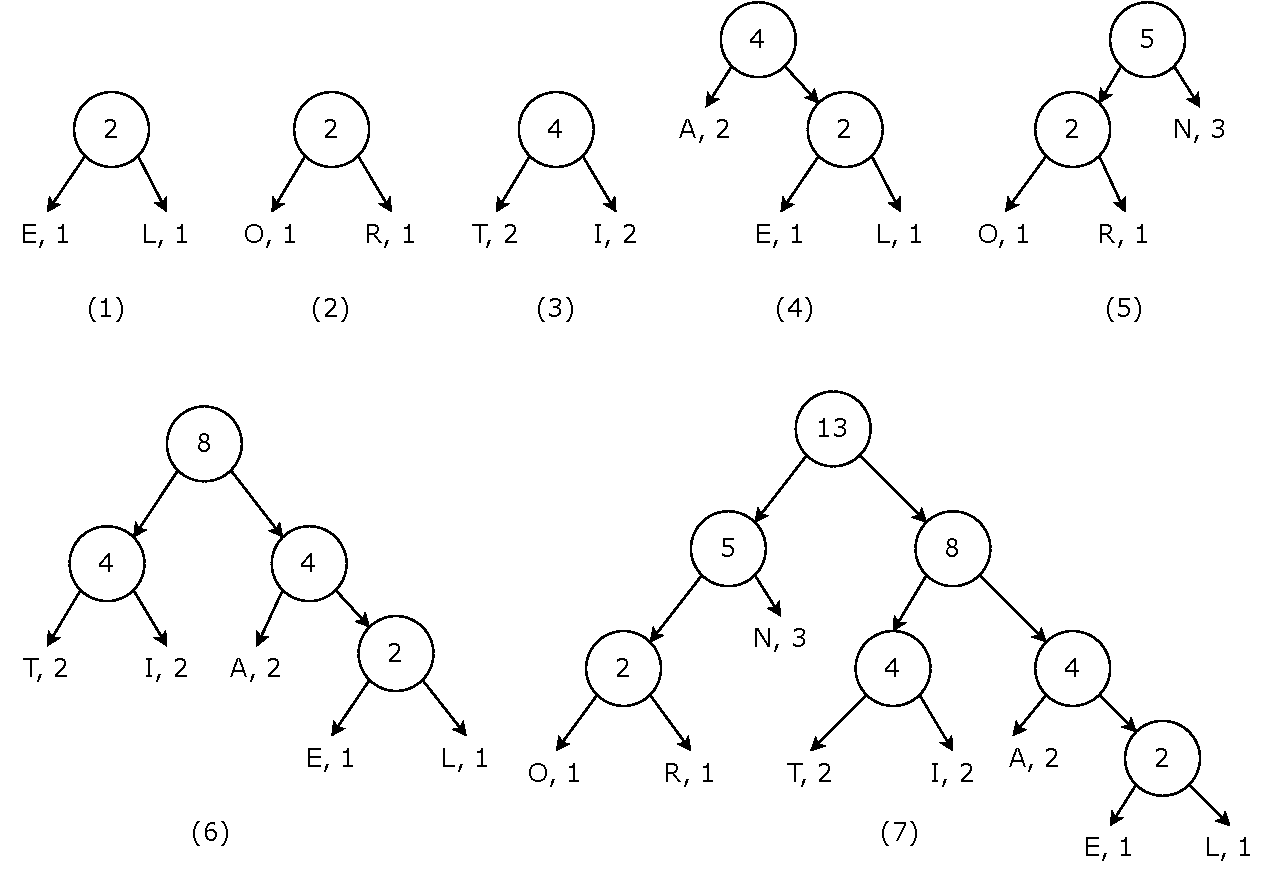
\includegraphics[scale=0.52]{img/huffman-steps}
  \caption{Build a Huffman tree.}
  \label{fig:huffman-build}
\end{figure}

We reuse the binary tree definition for Huffman tree. We augment the weight and only hold the symbol in leaf node. Let the branch node be $(w, l, r)$, where $w$ is the weight, $l$ and $r$ are the left and right sub-trees. Let the leaf be $(w, c)$, where $c$ is the symbol. When merge trees, we sum the weight: $merge\ a\ b\ = (weight\ a + weight\ b, a, b)$, where:

\be
\begin{array}{rcl}
weight\ (w, a) & = & w \\
weight\ (w, l, r) & = & w \\
\end{array}
\ee

Below function repeatedly pick and merge the minimum weighted trees:

\be
\begin{array}{rcl}
build\ [t] & = & t \\
build\ ts & = & build\ (merge\ t_1 t_2)\ ts', \text{where}: (t_1, t_2, ts') = extract\ ts
\end{array}
\ee

Function $extract$ picks two trees with minimal weight. Define $t_1 < t_2$ if $weight\ t_1 < weight\ t_2$.

\be
extract (t_1 \cons t_2 \cons ts) = foldr\ min_2\ (\min t_1\ t_2, \max t_1\ t_2, [\ ])\ ts
\ee

Where:

\be
min_2\ t\ (t_1, t_2, ts) = \begin{cases}
  t < t_2: & (\min\ t\ t_1, \max\ t\ t_1, t_2 \cons ts) \\
  \text{otherwise}: & (t_1, t_2, t \cons ts) \\
\end{cases}
\ee

To iterate building Huffman tree, we store $n$ sub-trees in array $A$. Scan $A$ from right to left, if the weight of $A[i]$ is less than $A[n-1]$ or $A[n]$, we swap $A[i]$ and \textproc{MAX}($A[n-1], A[n]$). Merge $A[n]$ and $A[n-1]$ after scan, and shrink the array by one. Repeat this to build the Huffman tree:

\begin{algorithmic}[1]
\Function{Huffman}{$A$}
  \While{$|A|>1$}
    \State $n \gets |A|$
    \For{$i \gets n - 2 $ down to $1$}
      \State $T \gets$ \Call{Max}{$A[n], A[n-1]$}
      \If{$A[i] < T$}
        \State \textproc{Exchange} $A[i]$ $\leftrightarrow T$
      \EndIf
    \EndFor
    \State $A[n-1] \gets$ \Call{Merge}{$A[n], A[n-1]$}
    \State \Call{Drop}{$A[n]$}
  \EndWhile
  \State \Return $A[1]$
\EndFunction
\end{algorithmic}

We can build the code table from the Huffman tree. Let $p = [\ ]$. Traverse from the root, update $p \gets 0 \cons p$ when go left; $p \gets 1 \cons p$ when go right. When arrive at leaf of symbol $c$, record $c \mapsto reverse\ p$ to the code table. Define (Curried form): $code\ = \textit{traverse}\ [\ ]$, where:

\be
\begin{array}{rcl}
\textit{traverse}\ p\ (w, c)\ & = & [c \mapsto reverse\ p] \\
\textit{traverse}\ p\ (w, l, r)\ & = & \textit{traverse}\ (0 \cons p)\ l \doubleplus \textit{traverse}\ (1 \cons p)\ l \\
\end{array}
\ee

When encoding, we scan the text $w$ while looking up the code table $dict$ to generate binary bits:

\be
encode\ dict\ w = \textit{concatMap}\ (c \mapsto dict[c])\ w, \text{where}: dict = code\ T
\ee

Conversely, when decoding, we scan the binary bits $bs$ while looking up the tree. Start from the root, go left for 0, right for 1; output symbol $c$ when arrive at leaf; then reset to the root to continue. $\textit{decode}\ T\ bs = lookup\ T\ bs$, where:

\be
\begin{array}{rcl}
lookup\ (w, c)\ [\ ] & = & [c] \\
lookup\ (w, c)\ bs & = & c : lookup\ T\ bs \\
lookup\ (w, l, r)\ (b \cons bs) & = & lookup\ (\text{if}\ b = 0\ \text{then}\ l\ \text{else}\ r)\ bs
\end{array}
\ee

Huffman tree building reflects a special strategy: always pick the two trees with the minimal weight for merge every time. The series of {\em local} optimal options generate a {\em global} optimal prefix-code. Local optimal sub-solutions are not necessary lead to global optimal solution usually. Huffman coding is an exception. We call the strategy that always choose the local optimal option as the {\em greedy} strategy. Greedy method simplifies and works for many problems. However, it's not easy to tell whether the greedy method generates the global optimal solution. The generic formal proof is still an active research area\cite{CLRS}.

\begin{Exercise}\label{ex:huffman-code}
\Question{Implement the imperative Huffman code table algorithm.}
\end{Exercise}

\begin{Answer}[ref = {ex:huffman-code}]
\Question{Implement the imperative Huffman code table algorithm.

\begin{Bourbaki}
data Node<T> {
    Optional<T> c = Nothing
    Int w
    Node<T> left = null, right = null

    Bool isLeaf() = (left == null and right == null)
}

Node<T> merge(Node<T> a, Node<T> b) = Node(Nothing, a.w + b.w, a, b)

Bool (<)(Node<T> a, Node<T> b) = (a.w < b.w)

Node<T> huffman([Node<T>] ts) {
    while length(ts) > 1 {
        Int n = length(ts)
        for Int i = n - 3 down to i 0 {
            if ts[i] < max(ts[n-1], ts[n-2]) {
                Int j = if ts[n-1] < ts[n-2] then n - 2 else n - 1
                swap(ts[i], ts[j])
            }
        }
        ts[n-2] = merge(ts[n-1], ts[n-2])
        ts.popLast()
    }
    return ts[0]
}

Map<T, [T]> codeTab(Node<T> t, [T] bits = [], Map<T, [T]> codes = {}) {
    if t.isLeaf() {
        codes[t.c] = bits
    } else {
        codeTab(t.left,  bits + [0], codes)
        codeTab(t.right, bits + [1], codes)
    }
    return codes
}
\end{Bourbaki}
}
\end{Answer}


\subsubsection{Change making problem}
\index{Change making problem}

How to change money with as few coins as possible? Suppose there are 5 values of coins: 1, 5, 25, 50, and 100. We define it as a set $C = \{1, 5, 25, 50, 100\}$. To change $x$ money, we can apply the greedy method, always choose the coin values most:

\be
\begin{array}{rcl}
change\ 0 & = & [\ ] \\
change\ x & = & c_m : change\ (x - c_m), \text{where}: c_m = \max\ \{c \in C, c \leq x\} \\
\end{array}
\ee

For example, to change 142 money, this function output a coin list: [100, 25, 5, 5, 5, 1, 1]. We can convert it to [(100, 1), (25, 1), (5, 3), (1, 2)], meaning 1 coin of 100, 1 coin of 25, 3 coins of 5, 2 coins of 1. For the coin system of $C$, the greedy method can find the optimal solution. Actually, it is applicable for most coin systems in the world. There are exceptions for example: $C = \{1, 3, 4 \}$. To change money $x = 6$, the optimal solution is 2 coins of 3, however, the greedy method gives 6 = 4 + 1 + 1, total 3 coins.

Although it's not the optimal solution, the greedy method often gives a simplified sub-optimal implementation. The result is often good enough in practice. For example, the word-wrap is a common functionality in editors. If the length of the text $T$ exceeds the page width $w$, we need break it into lines. Let the space between words be $s$, below greedy implementation gives the approximate optimal solution: put as many words as possible in a line.

\begin{algorithmic}[1]
\State $L \gets W$
\For{$w \in T$}
  \If{$|w| + s > L$}
    \State Insert line break
    \State $L \gets W - |w|$
  \Else
    \State $L \gets L - |w| - s$
  \EndIf
\EndFor
\end{algorithmic}

\begin{Exercise}\label{ex:huffman-build-tree}
\Question{Use heap to build the Huffman tree: take two trees from the top, merge then add back to the heap.}
\Question{If we sort the symbols by their weight as $A$, there is a linear time algorithm to build the Huffman tree: use a tree $Q$ to store the merge result, repeat take the minimal weighted tree from $Q$ and the head of $A$, merge then add to the queue. After process all trees in $A$, there is a single tree in the $Q$, which is the Huffman tree. Implement this algorithm.}
\Question{Given a Huffman tree $T$, implement the decode algorithm with fold left.}
\end{Exercise}

\begin{Answer}[ref = {ex:huffman-build-tree}]
\Question{Use heap to build the Huffman tree: take two trees from the top, merge then add back to the heap.

\[
\textit{Huffman}\ H = \begin{cases}
  H = \nil: & \nil \\
  |H| = 1: & pop\ H \\
  \text{otherwise}: & \textit{Huffman}\ (push\ (merge\ t_a\ t_b)\ H'') \\
\end{cases}
\]

Where: $(t_a, H') = pop\ H, (t_b, H'') = pop\ H'$

\begin{algorithmic}[1]
\Function{Huffman}{$H$}
  \While{$|H| > 1$}
    \State $t_a \gets$ \Call{Pop}{$H$}
    \State $t_b \gets$ \Call{Pop}{$H$}
    \State \textproc{Push}($H$, \Call{Merge}{$t_a, t_b$})
  \EndWhile
  \State \Return \Call{Pop}{$H$}
\EndFunction
\end{algorithmic}
}
\Question{If we sort the symbols by their weight as $A$, there is a linear time algorithm to build the Huffman tree: use a tree $Q$ to store the merge result, repeat take the minimal weighted tree from $Q$ and the head of $A$, merge then add to the queue. After process all trees in $A$, there is a single tree in the $Q$, which is the Huffman tree. Implement this algorithm.

$\textit{Huffman}\ (t \cons ts) = build\ (t, (ts, \nil))$, where:

\[
\begin{array}{rcl}
build\ (t, ([\ ], \nil)) & = & t \\
build\ (t, h) & = & build\ (extract\ (ts, push\ (merge\ t\ t')\ q)) \\
\end{array}
\]

where $(t', (ts, q)) = extract\ h$

\[
\begin{array}{rcl}
extract\ (t \cons ts, \nil)) & = & (t, (ts, \nil)) \\
extract\ ([\ ], q) & = & (t, ([\ ], q'), \text{where}: (t, q') = pop\ q \\
extract\ (t \cons ts, q) & = & \begin{cases}
  t' < t: & (t', (t \cons ts, q')), \text{where}: (t', q') = pop\ q \\
  t < t': & (t, (ts, q)) \\
  \end{cases}
\end{array}
\]

}
\Question{Given a Huffman tree $T$, implement the decode algorithm with fold left.

$decode = snd \circ (foldl\ lookup\ (T, [\ ]))$, where:

\[
\begin{array}{rcl}
lookup\ ((w, c), cs)\ b & = & (T, c \cons cs) \\
lookup\ ((w, l, r), cs)\ b & = & \text{if}\ b = 0\ \text{then}\ (l, cs)\ \text{else}\ (r, cs) \\
\end{array}
\]
}
\end{Answer}

\subsection{Dynamic programming}
\index{Dynamic programming}

Consider how to find the best solution to change money for any coin system. Let the best solution to change $x$ money is $C_m$ (the list of coins). We can partition $C_m$ into two groups: $C_1$ and $C_2$, with values $x_1$ and $x_2$ respectively, i.e., $C_m = C_1 \doubleplus C_2$ and $x = x_1 + x_2$. We'll prove that $C_1$ is the optimal solution to change $x_1$, and $C_2$ is the optimal solution to change $x_2$.

\begin{proof}
For $x_1$, suppose there exists another solution $C_1'$ with less coins
than $C_1$. Then the solution $C_1' \doubleplus C_2$ changes $x$ with less coins than $C_m$. This conflicts with the fact that $C_m$ is the optimal solution to change $x$. We can prove $C_2$ is the optimal solution to change $X_2$ in the same way.
\end{proof}

The reverse predication is not true. for any integer $y < x$, divide the original problem to two sub-problems: change $y$ and $x - y$. It's not necessary the overall optimal solution when combine the two optimal solutions. For example, use 3 values $C = \{1, 2, 4\}$ to change $x = 6$. The optimal solution needs two coins: $2 + 4$. As $6 = 3 + 3$, divide it to two same sub-problems of changing $3$. Each sub-problem has the optimal solution: $3 = 1 + $, however, the combination $(1 + 2) + (1 + 2)$ needs 4 coins. If an optimal problem can be divided into several sub optimal problems, we call it has optimal substructure. The change money problem has optimal substructure, but we need divide based on the coin value, but not an arbitrary integer.

\be
\begin{array}{rcl}
change\ 0 & = & [\ ] \\
change\ x & = & \min\ [c : change\ (x -c) | c \in C, c < x] \\
\end{array}
\ee

Where $\min$ picks the shortest list, However, this definition is impractical. There are too much duplicated computation. For example $C = \{1, 2, 25, 50, 100\}$, when computes $change(142)$, it needs further compute $change(141)$, $change(137)$, $change(117)$, $change(92)$, $change(42)$. For $change(141)$, minus it by 1, 2, 25, 50, 100, we go back to 137, 117, 92, 42. The search domain expands at $5^n$. Reuse the idea to generate Fibonacci numbers, we can use a table $T$ to records the optimal solution to the sub-problems. $T$ starts from empty. When change money $y$, we lookup $T[y]$ first. If $T[y] = \nil$, then recursively compute the sub-problem, then save the sub-solution in $T[y]$.

\begin{algorithmic}[1]
\State $T \gets [[\ ], \nil, \nil, ...]$ \Comment{$T[0] = [\ ]$}
\Function{Change}{$x$}
  \If{$x > 0$ and $T[x] = \nil$}
    \For{each $c$ in $C$ and $c \leq x$}
      \State $C_m \gets c :$ \Call{Change}{$x-c$}
      \If{$T[x] = \nil$ or $|C_m| < |T[x]|$}
        \State $T[x] \gets C_m$
      \EndIf
    \EndFor
  \EndIf
  \State \Return $T[x]$
\EndFunction
\end{algorithmic}

We can bottom-up generate optimal solutions for each sub-problem. From $T[0] = [\ ]$, generate $T[1] = [1]$, $T[2] = [1, 1]$, $T[3] = [1, 1, 1]$, $T[4] = [1, 1, 1, 1]$, as shown in \cref{tab:change-money}(a). There are two options for $T[5]$: 5 coins of 1, or a coin of 5. The latter need fewer coins. We update the optimal table to \cref{tab:change-money}(b), $T[5] = [5]$. Next change money $x = 6$. Both 1 and 5 are less than 6, there are two options: (1) 1 + $T[5]$ gives $[1, 5]$; (2) 5 + $T[1]$ gives $[5, 1]$. They are equivalent, we pick either $T[6] = [1, 5]$. For $T[i]$, where $i \leq x$, we check every coin value $c \leq i$. Lookup $T[i - c]$ for the sub-problem, then plus $c$ to get a new solution. We pick the fewest one as $T[i]$.

\begin{table}[htbp]
\centering
\begin{tabular}{|c||c|c|c|c|c|}
\hline
$x$ & 0 & 1 & 2 & 3 & 4 \\
\hline
optimal solution & $[\ ]$ & $[1]$ & $[1, 1]$ & $[1, 1, 1]$ & $[1, 1, 1, 1]$ \\
\hline
\end{tabular} \\
(a) Optimal solution for $x \leq 4$ \\
\vspace{10pt}
\begin{tabular}{c||c|c|c|c|c|c|}
\hline
$x$ & 0 & 1 & 2 & 3 & 4 & 5 \\
\hline
optimal solution & $[\ ]$ & $[1]$ & $[1, 1]$ & $[1, 1, 1]$ & $[1, 1, 1, 1]$ & $[5]$ \\
\hline
\end{tabular} \\
(b) Optimal solution for $x \leq 5$ \\
\caption{Optimal solution table}
\label{tab:change-money}
\end{table}

\begin{algorithmic}[1]
\Function{Change}{$x$}
  \State $T \gets [[\ ], \nil, ... ]$
  \For{$i \gets 1$ to $x$}
    \For{each $c$ in $C$ and $c \leq i$}
      \If{$T[i] = \nil$ or $1 + |T[i - c]| < |T[i]|$}
        \State $T[i] \gets  c : T[i-c]$
      \EndIf
    \EndFor
  \EndFor
  \State \Return $T[x]$
\EndFunction
\end{algorithmic}

There are many duplicated content in the optimal solution table as below. A solution contains the sub-solutions. We can only record the changed part: the coin $c$ we chosen for $T[i]$ and the number $n$ of coins, i.e., $T[i] = (n, c)$. To generate the list of coins for $x$, we lookup $T[x]$ to get $c$, then lookup $T[x - c]$ to get $c'$, ... repeat this to $T[0]$.

\btab{|c||c|c|c|c|c|c|}
\hline
value & 6 & 7 & 8 & 9 & 10 & ... \\
\hline
optimal solution & $[1, 5]$ & $[1, 1, 5]$ & $[1, 1, 1, 5]$ & $[1, 1, 1, 1, 5]$ & $[5, 5]$ & ... \\
\hline
\etab

\begin{algorithmic}[1]
\Function{Change}{$x$}
  \State $T \gets [(0, \nil), (\infty, \nil), (\infty, \nil), ... ]$
  \For{$i \gets 1$ to $x$}
    \For{each $c$ in $C$ and $c \leq i$}
      \State $(n, \_) \gets T[i - c], (m, \_) \gets T[i]$
      \If{$1 + n < m$}
        \State $T[i] \gets (1 + n, c)$
      \EndIf
    \EndFor
  \EndFor
  \State $s \gets [\ ]$
  \While{$x > 0$}
    \State $(\_, c) \gets T[x]$
    \State $s \gets c : s$
    \State $x \gets x - c$
  \EndWhile
  \State \Return $s$
\EndFunction
\end{algorithmic}

We can build the optimal solution table $T$ with left fold: $\textit{foldl}\ fill\ [(0, 0)]\ [1, 2, ...]$, where:

\be
fill\ T\ x = T \rhd \min\ \{(\textit{fst}\ T[x - c], c) | c \in C, c \leq x\}
\ee

Where $s \rhd a$ append $a$ to the right of $s$ (see finger tree in chapter 12). Then rebuild the optimal solution backwards from $T$:

\be
\begin{array}{rcl}
change\ 0\ T & = & [\ ] \\
change\ x\ T & = & c : change\ (x - c)\ T, \text{where}: c = \textit{snd}\ T[x] \\
\end{array}
\ee

For $x = n$, we loop $n$ times, check at most $k = |C|$ coins. The performance is bound to $\Theta(nk)$\footnote{upper bound}, and need $O(n)$ space to persist $T$ both in the top-down and bottom-up implementations. The solution to the sub-problem is used many times to compute the global optimal solution. We call it overlapping sub-problems. Richard Bellman developed dynamic programming in 1940s. It has two properties.

\begin{enumerate}
\item Optimal sub-structure. The problem can be broken down into small problems. The optimal solution can be constructed from the solutions of these sub-problems;
\item Overlapping sub-problems. The solution of the sub-problem is reused multiple times to find the overall solution.
\end{enumerate}

\subsubsection{Longest common sub-sequence}
\index{LCS} \index{Longest common sub-sequence}

Different with sub-string, the sub-sequence needn't be consecutive. For example: the longest common sub-string of `Mississippi' and `Missunderstanding' is `Miss', while the longest common sub-sequence is `Misssi' as shown in \cref{fig:lcs}. If rotate the figure by 90\degree, it turns to be a `diff' result between them. This is a common function in version control tools. The longest common sub-sequence of $x$ and $y$ are defined as below:

\begin{figure}[htbp]
 \centering
 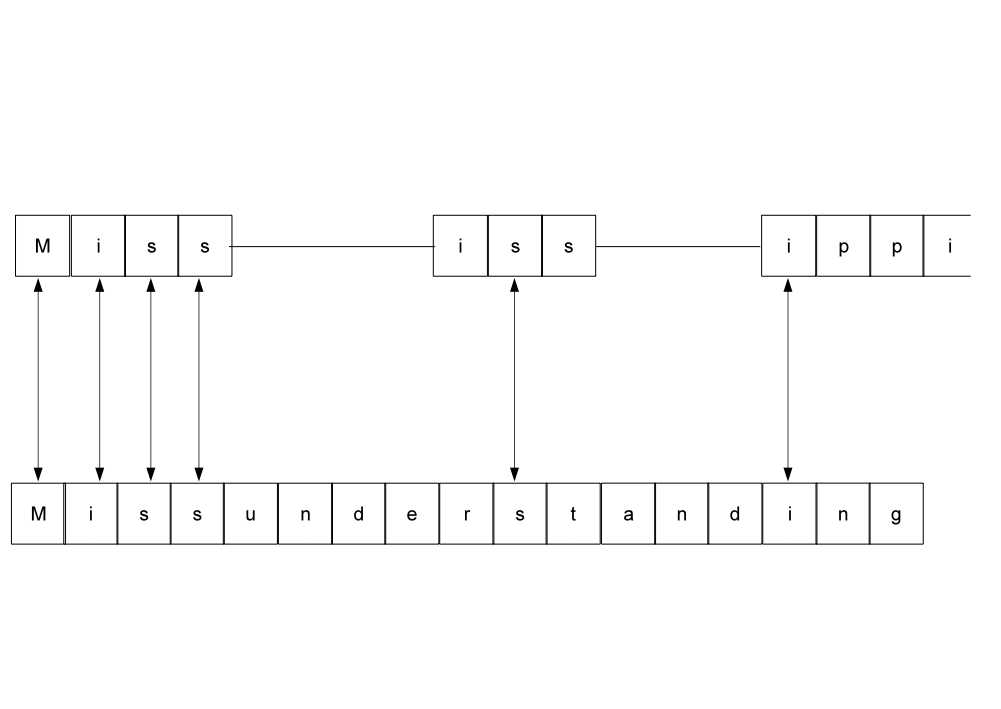
\includegraphics[scale=0.6]{img/lcs}
 \caption{The longest common sub-sequence}
 \label{fig:lcs}
\end{figure}

\be
\begin{array}{rcl}
LCS([\ ], ys) & = & [\ ] \\
LCS(xs, [\ ]) & = & [\ ] \\
LCS(x \cons xs, y \cons ys) & = & \begin{cases}
  x = y: & x : LCS(xs, ys) \\
  \text{otherwise}: & \max\ LCS(x \cons xs, ys)\ LCS(xs, y \cons ys)
  \end{cases}
\end{array}
\ee

Where $\max$ picks the longer sequence. There is optimal sub-structure in the definition of $LCS$. It can be broken down into sub-problems. The sequence length reduced at least by 1 every time. There are overlapping sub-problems. The longest common sub-sequence of the sub-strings are reused multiple times to find the global optimal solution. We use a 2D table $T$ to record the optimal solution of the sub-problems. The row and column represent $xs$ and $ys$ respectively. Index the sequence from 0. Row 0, column 0 represents the empty sequence. $T[i][j]$ is the length of $LCS(xs[0..j], ys[0..i])$. We finally build the longest common sub-sequences from $T$. Because $LCS([\ ], ys) = LCS(xs, [\ ]) = [\ ]$, row 0 and column 0 are all 0s. Consider `antenna' and `banana' for example, we fill row 1 from $T[1][1]$. `b' is different from any one in `antenna', hence row 1 are all 0s. For $T[2][1]$, the row and column are corresponding to `a', $T[2][1] = T[1][0] + 1 = 1$, i.e., $LCS(\text{a}, \text{ba}) = \text{a}$. Next move to $T[2][2]$, `a' $neq$ `n', we choose the greater one between the above ($LCS(\text{an}, \text{b})$) and the left ($LCS(\text{a}, \text{ba})$) as $T[2][2]$, which equals to 1, i.e., $LCS(\text{ba}, \text{an}) = \text{a}$. In this way, we step by step fill the table out. The rule is: for $T[i][j]$, if $xs[i-1] = ys[i-1]$, then $T[i][j] = T[i-1][j-1] + 1$; otherwise, pick the greater one from above $T[i-1][j]$ and the left $T[i][j-1]$.

\btab{|c|c|c|c|c|c|c|c|c|c|}
\hline
    &     & 0  & 1 & 2 & 3 & 4 & 5 & 6 & 7 \\
\hline
   &    & [\ ] & a & n & t & e & n & n & a \\
\hline
0 & [\ ] & 0   & 0 & 0 & 0 & 0 & 0 & 0 & 0 \\
\hline
1 &  b   & 0   & 0 & 0 & 0 & 0 & 0 & 0 & 0 \\
\hline
2 &  a   & 0   & 1 & 1 & 1 & 1 & 1 & 1 & 1 \\
\hline
3 &  n   & 0   & 1 & 2 & 2 & 2 & 2 & 2 & 2 \\
\hline
4 &  a   & 0   & 1 & 2 & 2 & 2 & 2 & 2 & 3 \\
\hline
5 &  n   & 0   & 1 & 2 & 2 & 2 & 3 & 3 & 3 \\
\hline
6 &  a   & 0   & 1 & 2 & 2 & 2 & 3 & 3 & 4 \\
\hline
\etab

\begin{algorithmic}[1]
\Function{LCS}{$xs, ys$}
  \State $m \gets |xs|, n \gets |ys|$
  \State $T \gets [[0, 0, ...], [0, 0, ...], ...]$ \Comment{$(m+1) \times (n+1)$}
  \For{$i \gets 1$ to $m$}
    \For{$j \gets 1$ to $n$}
      \If{$xs[i] = ys[j]$}
        \State $T[i+1][j+1] \gets T[i][j] + 1$
      \Else
        \State $T[i+1][j+1] \gets$ \Call{Max}{$T[i][j+1], T[i+1][j]$}
      \EndIf
    \EndFor
  \EndFor
  \State \Return \Call{Fetch}{$T, xs, ys$}  \Comment{build the LCS}
\EndFunction
\end{algorithmic}

We next build the longest common sub-sequence from $T$. Start from the bottom-right, if $xs[m] = ys[n]$, then $xs[m]$ is the tail of the LCS, we next compare $xs[m-1]$ and $ys[n-1]$; otherwise, we pick the greater one from $T[m-1][n]$ and $T[m][n-1]$ and go on.

\begin{algorithmic}[1]
\Function{Fetch}{$T, xs, ys$}
  \State $m \gets |xs|, n \gets |ys|$
  \State $r \gets [\ ]$
  \While{$m > 0$ and $n > 0$}
    \If{$xs[m - 1] = ys[n - 1]$}
      \State $r \gets xs[m - 1] : r$
      \State $m \gets m - 1$
      \State $n \gets n - 1$
    \ElsIf{$T[m - 1][n] > T[m][n - 1]$}
      \State $m \gets m - 1$
    \Else
      \State $n \gets n - 1$
    \EndIf
  \EndWhile
  \State \Return $r$
\EndFunction
\end{algorithmic}

\begin{Exercise}\label{ex:lcs}
\Question{For the longest common sub-sequence, build the optimal solution table with fold.}
\end{Exercise}

\begin{Answer}[ref={ex:lcs}]
\Question{For the longest common sub-sequence, build the optimal solution table with fold.

\begin{Haskell}
import Data.Sequence (Seq, singleton, fromList, index, (|>))

lcs xs ys = construct $ foldl f (singleton $ fromList $ replicate (n+1) 0)
                               (zip [1..] xs) where
  (m, n) = (length xs, length ys)
  f tab (i, x) = tab |> (foldl longer (singleton 0) (zip [1..] ys)) where
    longer r (j, y) = r |> if x == y
                    then 1 + (tab `index` (i-1) `index` (j-1))
                    else max (tab `index` (i-1) `index` j) (r `index` (j-1))
  construct tab = get (reverse xs, m) (reverse ys, n) where
    get ([], 0) ([], 0) = []
    get ((x:xs), i) ((y:ys), j)
      | x == y = get (xs, i-1) (ys, j-1) ++ [x]
      | (tab `index` (i-1) `index` j) > (tab `index` i `index` (j-1)) =
                 get (xs, i-1) ((y:ys), j)
      | otherwise = get ((x:xs), i) (ys, j-1)
\end{Haskell}
}
\end{Answer}

\subsubsection{Subset sum}
\index{Subset sum}

Given a set $X$ of integers, how to find all the subsets $S \subseteq X$, that the sum of elements in $S$ is $s$, i.e., $\sum S = \sum\limits_{i \in S} i = s$? For example, $X$ = \{11, 64, -82, -68, 86, 55, -88, -21, 51\}, there are three subsets with sum $s = 0$: $S = \varnothing$, \{64, -82, 55, -88, 51\}, \{64, -82, -68, 86\}. We need exhaust $2^n$ subset sums, where $n = |X|$, the performance is $O(n 2^n)$.

\be
\begin{array}{rcl}
sets\ s\ \nil & = & [\nil] \\
sets\ s\ (x \cons xs) & = & \begin{cases}
  s = x: & \{ x \} : sets\ s\ xs \\
  \text{otherwise}: & (sets\ s\ xs) \doubleplus [x \cons S | S \in sets\ (s - x)\ xs] \\
  \end{cases}
\end{array}
\ee

There is sub-structure and overlapping sub-problems in above exhaustive search definition, we can apply dynamic programming method. We bottom-up build solution table $T$, and generate the final subset. First consider the existence of some subset $S$, satisfying $\sum S = s$. We scan the elements to determine the bottom/up bound of the subset sum $l \leq s \leq u$. if $s < l$ or $s > u$, then there's no solution.

\be
  l = \sum \{x \in X, x < 0\}, u = \sum \{x \in X, x > 0\}
\ee

As the elements are integers, there are $m = u - l + 1$ columns in table $T$, each corresponds to a value: $l \leq j \leq u$. There are $n = |X| + 1$ rows, each corresponds to some element $x_i$. $T[i][j]$ indicates whether exists some subset $S \subseteq \{x_1, x_2, ..., x_i\}$, satisfying $\sum S = j$. Row 0 is special, represents the sum of empty set $\varnothing$. All entries in $T$ start from false F except $T[0][0] =$ T, meaning $\sum \varnothing = 0$. Start from $x_1$ to build row 1. Besides $\sum \varnothing = 0$, $\sum \{x_1\} = x_1$, hence $T[1][0] = $T, $T[1][x_1] = $T.

\btab{|c|c|c|c|c|c|c|c|c|}
\hline
 & $l$ & $l+1$ & ... & 0 & ... &$x_1$ & ... & $u$ \\
\hline
$\varnothing$ & F & F & ... & T & ... & F & ... & F \\
\hline
$x_1$ & F & F & ... & T & ... &T & ... & F \\
\hline
... & F & F & ... & T & ... & T & ... & F \\
\etab

Add $x_2$, we get 4 possible subset sums: $\sum \varnothing = 0$, $\sum \{x_1\} = x_1$, $\sum \{x_2\} = x_2$, $\sum \{x_1, x_2\} = x_1 + x_2$.

\btab{|c|c|c|c|c|c|c|c|c|c|c|c|c|}
\hline
 & $l$ & $l+1$ & ... & 0 & ... & $x_1$ & ... & $x_2$ & ... & $x_1 + x_2$ & ... & $u$ \\
\hline
$\varnothing$ & F & F & ... & T & ... & T & ... & F & ... & F & ... & F \\
\hline
$x_1$ & F & F & ... & T & ... & T & ... & F & ... & F & ... & F \\
\hline
$x_2$ & F & F & ... & T & ... & T & ... & T & ... & T & ... & F \\
\hline
... & F & F & ... & T & ... & T & ... & T & ... & T & ... & F \\
\etab

We add element $x_i$ to fill row $i$. We can obtain all subset sums from previous elements: $\{x_1, x_2, ..., x_{i-1}\}$, hence all the entries of true in previous row are still true. Because $\sum \{x_i\} = x_i$, hence $T[i][x_i] =$ T. We add $x_i$ to each previous sum, generate some new sums, the corresponding entries of them are all true. After add all $n$ elements, the Boolean value of $T[n][s]$ gives whether the subset sum $s$ exists.

\begin{algorithmic}[1]
\Function{Subset-Sum}{$X, s$}
  \State $l \gets \sum \{x \in X, x < 0\}, u \gets \sum \{x \in X, x > 0\}$
  \State $n \gets |X|$
  \State $T \gets \{\{\text{F}, \text{F}, ...\}, \{\text{F}, \text{F}, ...\}, ...\}$ \Comment{$(n+1) \times (u - l + 1)$}
  \State $T[0][0] \gets$ T   \Comment{$\sum \varnothing = 0$}
  \For{$i \gets 1$ to $n$}
    \State $T[i][X[i]] \gets $T
    \For{$j \gets l$ to $u$}
      \State $T[i][j] \gets T[i][j] \lor T[i-1][j]$
      \State $j' \gets j - X[i]$
      \If{$l \leq j' \leq u$}
        \State $T[i][j] \gets T[i][j] \lor T[i-1][j']$
      \EndIf
    \EndFor
  \EndFor
  \State \Return $T[n][s]$
\EndFunction
\end{algorithmic}

The column index $j$ does not start from 0, but from $l$ to $u$. We can convert it by $j - l$ in programming environment. We next generate all subsets $S$ satisfying $\sum S = s$ from table $T$. If $T[n][s] =$F then there's no solution; otherwise, there are two cases: (1) if $x_n = s$, then the singleton set $\{x_n\}$ is a solution. We next lookup $T[n - 1][s]$, if it's true $T$, then recursively generate all subsets from $\{x_1, x_2, x_3, ..., x_{n-1}\}$ that the sum is $s$. (2) let $s' = s - x_n$, if $l \leq s' \leq u$ and $T[n - 1][s']$ is true, we recursively generate subsets from $\{x_1, x_2, x_3, ..., x_{n-1}\}$ that the sum is $s'$, then add $x_n$ to each subset.

\begin{algorithmic}[1]
\Function{Get}{$X, s, T, n$}
  \State $r \gets [\ ]$
  \If{$X[n] = s$}
    \State $r \gets \{X[n]\} : r$
  \EndIf
  \If{$n > 1$}
    \If{$T[n-1][s]$}
      \State $r \gets r \doubleplus $ \Call{Get}{$X, s, T, n-1$}
    \EndIf
    \State $s' \gets s - X[n]$
    \If{$l \leq s' \leq u$ and $T[n-1][s']$}
      \State $r \gets r \doubleplus [(X[n] \cons r') | r' \gets $ \Call{Get}{$X, s', T, n-1$} $]$
    \EndIf
  \EndIf
  \State \Return $r$
\EndFunction
\end{algorithmic}

The dynamic programming method loops $O(n(u - l + 1))$ times to build table $T$, then recursively generate the solution in $O(n)$ levels. The 2D table need $O(n(u - l + 1))$ space. We can replace it with a 1D vector $V$ of $u - l + 1$ entries. each $V[j] = \{S_1, S_2, ...\}$ stores the subsets that $\sum S_1 = \sum S_2 = ... = j$. $V$ start from all empty entries. For each $x_i$, we update $V$ a round, add the new obtained sums with $x_i$. The final solution is in $V[s]$.

\begin{algorithmic}[1]
\Function{Subset-Sum}{$X, s$}
  \State $l \gets \sum \{x \in X, x < 0\}, u \gets \sum \{x \in X, x > 0\}$
  \State $V \gets [\nil, \nil, ...]$   \Comment{$u - l + 1$}
  \For{each $x$ in $X$}
    \State $U \gets$ \Call{Copy}{$V$}
    \For{$j \gets l$ to $u$}
      \If{$x = j$}
        \State $U[j] \gets \{\{x\}\} \cup U[j]$
      \EndIf
      \State $j' \gets j - x$
      \If{$l \leq j' \leq u$ and $V[j'] \neq \nil$}
        \State $U[j] \gets U[j] \cup \{(\{x\} \cup S) | S \in V[j']\}$
      \EndIf
    \EndFor
    \State $V \gets U$
  \EndFor
  \State \Return $V[s]$
\EndFunction
\end{algorithmic}

We can build the solution vector with left fold: $V = foldl\ bld\ (replicate (u - l + 1)\ \nil)\ X$, where $\textit{replicate}\ n\ a$ generates list $[a, a, ..., a]$ of length $n$. $bld$ updates $V$ with each elements in $X$.

\be
bld\ V\ x = foldl\ f\ V\ [l, l + 1..., u]
\ee

Where:

\be
f\ V\ j = \begin{cases}
  j = x: & V[j] \cup \{\{x\}\} \\
  l \leq j' \leq u\ \text{and}\ T[j'] \neq \nil: & V[j] \cup \{ \{x\} S | S \in T[j']\}, \text{where}: j' = j - x \\
  \text{otherwise}: & V
  \end{cases}
\ee

\begin{Exercise}\label{ex:dynamic-programming}
\Question{For the longest common sub-sequence problem, an alternative solution is to record the length and the direction in the table. There are three directions: 'N' for north, 'W' for west, and 'NW'. Given such a table, we can build the longest common sub-sequence from the bottom-right entry. If the entry is 'NW', next go to the upper-left entry; if it's 'N', go to the above row; and go to the previous entry if it's 'W'. Implement this solution.}
\Question{For the subset sum upper/lower bound, does $l \leq 0 \leq u$ always hold? can we reduce the range between the bounds?}
\Question{Given a list of non-negative integers, find the maximum sum composed by numbers that none of them are adjacent.
% refer to others/problems/DP/non-adjcent-sum/
}
\Question{Edit distance (also known as Levenshtein edit distance) is defined as the cost of converting from one string $s$ to another string $t$. It is widely used in spell-checking, OCR correction etc. There are three symbol changes: insert, delete, and replace. Each operation mutate a character a time. For example the edit distance is 3 for `kitten' $\mapsto$ `sitting':
  \begin{enumerate}
  \item \textbf{k}itten $\rightarrow$ \textbf{s}itten (k $\mapsto$ s);
  \item sitt\textbf{e}n $\rightarrow$ sitt\textbf{i}n (e $\mapsto$ i);
  \item sittin $\rightarrow$ sittin\textbf{g} (+ g).
  \end{enumerate}
Compute the edit distance with dynamic programming.}
\end{Exercise}

\begin{Answer}[ref = {ex:dynamic-programming}]
\Question{For the longest common sub-sequence problem, an alternative solution is to record the length and the direction in the table. There are three directions: 'N' for north, 'W' for west, and 'NW'. Given such a table, we can build the longest common sub-sequence from the bottom-right entry. If the entry is 'NW', next go to the upper-left entry; if it's 'N', go to the above row; and go to the previous entry if it's 'W'. Implement this solution.

\begin{Bourbaki}
data DIR = N | W | NW

[K] lcs([K] xs, [K] ys) {
    Int m = length(x), n = length(ys)
    [[(Int, DIR)]] c = [[(0, null)] * (n + 1)] * (m + 1)
    for i = 1 to m {
        for j = 1 to n {
            if xs[i-1] == ys[j-1] {
                c[i][j] = (fst(c[i-1][j-1]) + 1, DIR.NW)
            } else {
                c[i][j] = if fst(c[i-1][j]) > fst(c[i][j-1])
                    then (fst(c[i-1][j]), DIR.N)
                    else (fst(c[i][j-1]), DIR.W)
            }
        }
    }
    return rebuild(c, xs, ys)
}

[K] rebuild([[(Int, DIR)]] c, [K] xs, [K] ys) {
    [K] r = []
    Int m = length(xs), n = length(ys)
    while m > 0 and n > 0 {
        DIR d = snd(c[m][n])
        if d == DIR.NW {
            r.append(xs[m - 1]) // or ys[n - 1]
            m = m - 1, n = n - 1
        } else if d == DIR.N {
            m = m - 1
        } else if d == DIR.W {
            n = n - 1
        }
    }
    return reverse(r)
}
\end{Bourbaki}
}
\Question{For the subset sum upper/lower bound, does $l \leq 0 \leq u$ always hold? can we reduce the range between the bounds?

For non-empty subset (the sum of empty is 0), $l \leq 0 \leq u$ does not hold necessarily. Consider set $X$ of only positive numbers, the lower bound can't be less than 0, and $l = \min(X)$. For set of only negative numbers, the upper bound can't be greater than 0, and $u = \max(X)$.
}
\Question{Compute the edit distance between two strings.

\begin{Bourbaki}
Int lev([K] s, [K] t) {
    [[Int]] d = [[0]*n]*m   //d[i][j]: distance between s[:i] and t[:j]
    for Int i = 0 to length(s) {
        d[i][0] = i  //drop all chars of source prefix gives []
    }
    for Int j = 0 to length(t) {
        d[0][j] = j  //insert all chars of target prefix to []
    }
    for Int j = 1 to length(t) {
        for i = 1 to length(m) {
            c = if s[i-1] == t[j-1] then 0 else 1
            d[i][j] = min([d[i-1][j] + 1,    //deletion
                           d[i][j-1] + 1,    //insertion
                           d[i-1][j-1] + c]) //substitution
        }
    }
    return d[length(s)][length(t)]
}
\end{Bourbaki}
}
\end{Answer}

\section{Appendix - example programs}

Find the top-$k$ element:

\begin{lstlisting}[language = Bourbaki]
Optional<K> top(Int k, [K] xs, Int l, Int u) {
    if l < u {
        swap(xs, l, rand(l, u))
        var p = partition(xs, l, u)
        if p - l + 1 == k
            return Optional.of(xs[p])
        return if k < p - l + 1 then top(k, xs, l, p)
               else top(k- p + l - 1, xs, p + 1, u)
    }
    return Optional.Nothing
}

Int partition([K] xs, Int l, Int u) {
    var p = l
    for var r = l + 1 to u {
        if not xs[p] < xs[r] {
            l = l + 1
            swap(xs, l, r)
        }
    }
    swap(xs, p, l)
    return l
}
\end{lstlisting}

Saddle back search:

\begin{Haskell}
solve f z = search 0 m where
  search p q | p > n || q < 0 = []
             | z' < z = search (p + 1) q
             | z' > z = search p (q - 1)
             | otherwise = (p, q) : search (p + 1) (q - 1)
    where z' = f p q
  m = bsearch (f 0) z (0, z)
  n = bsearch (\x->f x 0) z (0, z)

bsearch f y (l, u) | u <= l = l
                   | f m <= y = if f (m + 1) <= y then bsearch f y (m + 1, u) else m
                   | otherwise = bsearch f y (l, m-1)
  where m = (l + u) `div` 2
\end{Haskell}

Boyer-Moore majority:

\begin{lstlisting}[language = Bourbaki]
Optional<T> majority([T] xs) {
    var (m, c) = (Optional<T>.Nothing, 0)
    for var x in xs {
        if c == 0 then (m, c) = (Optional.of(x), 0)
        if x == m then c++ else c--
    }
    c = 0
    for var x in xs {
        if x == m then c++
    }
    return if c > length(xs)/2 then m else Optional<T>.Nothing
}
\end{lstlisting}

Find the majority with fold:

\begin{Haskell}
majority xs = verify $ foldr maj (Nothing, 0) xs where
  maj x (Nothing, 0) = (Just x, 1)
  maj x (Just y, v) | x == y = (Just y, v + 1)
                    | v == 0 = (Just x, 1)
                    | otherwise = (Just y, v - 1)
  verify (Nothing, _) = Nothing
  verify (Just m, _)  = if 2 * (length $ filter (==m) xs) > length xs
                        then Just m else Nothing
\end{Haskell} %$

The maximum sum of sub-vector:

\begin{Haskell}
maxSum :: (Ord a, Num a) => [a] -> a
maxSum = fst . foldr f (0, 0) where
  f x (m, mSofar) = (m', mSofar') where
    mSofar' = max 0 (mSofar + x)
    m' = max mSofar' m
\end{Haskell}

KMP string matching:

\begin{lstlisting}[language = Bourbaki]
[Int] match([T] w, [T]p) {
    n = length(w), m = length(p)
    [Int] fallback = prefixes(p)
    [Int] r = []
    Int k = 0
    for i = 0 to n {
        while k > 0 and p[k] != w[i] {
            k = fallback[k]
        }
        if p[k] == w[i] then k = k + 1
        if k == m {
            add(r, i + 1 - m)
            k = fallback[k - 1]
        }
    }
    return r
}

[Int] prefixes([T] p) {
    m = length(p)
    [Int] t = [0] * m  //fallback table
    Int k = 0
    for i = 2 to m {
        while k > 0 and p[i-1] != p[k] {
            k = t[k-1] #fallback
        }
        if p[i-1] == p[k] then k = k + 1
        t[i] = k
    }
    return t
}
\end{lstlisting}

%% 鲍耶-摩尔字符串匹配算法:

%% \begin{lstlisting}[language = Bourbaki]
%% [Int] bmMatch([T] w, [T] p) {
%%     n = length(w), m = length(p)
%%     tab1 = badChar(p)
%%     tab2 = goodSuffix(p)
%%     res = []
%%     offset = 0
%%     while offset + m <= n {
%%         i = m - 1
%%         while i >= 0 and p[i] == w[offset + i] {
%%             i = i - 1
%%         }
%%         if i < 0 {
%%             append(res, offset)
%%             offset = offset + 1
%%         } else {
%%             offset = offset + max(tab1[w[offset + m - 1]], tab2[i])
%%         }
%%     }
%%     return res
%% }

%% Map<T, Int> badChar([T] p) {
%%     m = length(p)
%%     tab = mapOf(T.values, m)
%%     for i = 0 to m - 2 {
%%         tab[p[i]] = m - 1 - i
%%     }
%%     return tab
%% }

%% [Int] goodSuffix(p) {
%%     m = len(p)
%%     tab = [0] * m
%%     Int last = 0
%%     for i = m - 1 down to 1 {
%%         if isPrefix(p, i) then last = i
%%         tab[i - 1] = last
%%     }
%%     for i = 0 to m - 1 {
%%         slen = suffixLen(p, i)
%%         if slen != 0 and p[i - slen] != p[m - 1 - slen] {
%%             tab[m - 1 - slen] = m - 1 - i
%%         }
%%     }
%%     return tab
%% }

%% // if p[i..m-1] `is prefix of` p
%% Bool isPrefix([T] p, Int i) {
%%     for j = 0 to length(p) - i - 1 {
%%         if p[j] != p [i+j] then return False
%%     }
%%     return True
%% }

%% // length of the longest suffix of p[..i], which is also a suffix of p
%% Int suffix_len([T] p, Int i) {
%%     m = length(p)
%%     Int j = 0
%%     while p[m - 1 - j] == p[i - j] and j < i {
%%         j = j + 1
%%     }
%%     return j
%% }
%% \end{lstlisting}

The maze puzzle:

\begin{Haskell}
dfsSolve m from to = solve [[from]] where
  solve [] = []
  solve (c@(p:path):cs)
      | p == to = reverse c
      | otherwise = let os = filter (`notElem` path) (adj p) in
                      if os == [] then solve cs
                      else solve ((map (:c) os) ++ cs)
  adj (x, y) = [(x', y') | (x', y') <- [(x-1, y), (x+1, y), (x, y-1), (x, y+1)],
                           inRange (bounds m) (x', y'), m ! (x', y') == 0]
\end{Haskell}

The eight queens puzzle:

\begin{Haskell}
solve = dfsSolve [[]] [] where
  dfsSolve [] s = s
  dfsSolve (c:cs) s
           | length c == 8 = dfsSolve cs (c:s)
           | otherwise = dfsSolve ([(x:c) | x <- [1..8] \\ c,
                             not $ attack x c] ++ cs) s
  attack x c = let y = 1 + length c in
                any (\(i, j) -> abs(x - i) == abs(y - j)) $
                    zip (reverse c) [1..]
\end{Haskell}

The peg puzzle:

\begin{Haskell}
solve = dfsSolve [[[-1, -1, -1, 0, 1, 1, 1]]] [] where
    dfsSolve [] s = s
    dfsSolve (c:cs) s
             | head c == [1, 1, 1, 0, -1, -1, -1] = dfsSolve cs (reverse c:s)
             | otherwise = dfsSolve ((map (:c) $ moves $ head c) ++ cs) s

moves s = filter (/=s) [leapLeft s, hopLeft s, leapRight s, hopRight s] where
    leapLeft [] = []
    leapLeft (0:y:1:ys) = 1:y:0:ys
    leapLeft (y:ys) = y:leapLeft ys
    hopLeft [] = []
    hopLeft (0:1:ys) = 1:0:ys
    hopLeft (y:ys) = y:hopLeft ys
    leapRight [] = []
    leapRight (-1:y:0:ys) = 0:y:(-1):ys
    leapRight (y:ys) = y:leapRight ys
    hopRight [] = []
    hopRight (-1:0:ys) = 0:(-1):ys
    hopRight (y:ys) = y:hopRight ys
\end{Haskell}

Iterative solution to the peg puzzle:

\begin{lstlisting}[language = Bourbaki]
[Int] solve([Int] start, [Int] end) {
    stack = [[start]]
    s = []
    while stack != [] {
        c = pop(stack)
        if c[0] == end {
            s += reverse(c)
        } else {
            for [Int] m in moves(c[0]) {
                stack += (m:c)
            }
        }
    }
    return s
}

[[Int]] moves([Int] s) {
    [[Int]] ms = []
    n = length(s)
    p = find(s, 0)
    if p < n - 2 and s[p+2] > 0 then ms += swap(s, p, p+2)
    if p < n - 1 and s[p+1] > 0 then ms += swap(s, p, p+1)
    if p > 1 and s[p-2] < 0 then ms += swap(s, p, p-2)
    if p > 0 and s[p-1] < 0 then ms += swap(s, p, p-1)
    return ms
}

[Int] swap([Int] s, Int i, Int j) {
    a = copy(s)
    (a[i], a[j]) = (a[j], a[i])
    return a
}
\end{lstlisting}

The wolf, goat, cabbage cross river puzzle:

\begin{Haskell}
import Data.Bits
import qualified Data.Sequence as Queue
import Data.Sequence (Seq((:<|)), (><))

solve = bfsSolve $ Queue.singleton [(15, 0)] where
  bfsSolve Queue.Empty = [] -- no solution
  bfsSolve (c@(p:_) :<| cs)
    | fst p == 0 = reverse c
    | otherwise = bfsSolve (cs >< (Queue.fromList $ map (:c)
                                    (filter (`valid` c) $ moves p)))

valid (a, b) r = not $ or [ a `elem` [3, 6], b `elem` [3, 6], (a, b) `elem` r]

moves (a, b) = if b < 8 then trans a b else map swap (trans b a) where
    trans x y = [(x - 8 - i, y + 8 + i)
                     | i <-[0, 1, 2, 4], i == 0 || (x .&. i) /= 0]
    swap (x, y) = (y, x)
\end{Haskell}

The extended Euclid algorithm to solve the water jugs puzzle:

\begin{Haskell}
extGcd 0 b = (b, 0, 1)
extGcd a b = let (d, x', y') = extGcd (b `mod` a) a in
               (d, y' - x' * (b `div` a), x')

solve a b g | g `mod` d /= 0 = []
            | otherwise = solve' (x * g `div` d)
    where
      (d, x, y) = extGcd a b
      solve' x | x < 0 = solve' (x + b)
               | otherwise = pour x [(0, 0)]
      pour 0 ps = reverse ((0, g):ps)
      pour x ps@((a', b'):_) | a' == 0 = pour (x - 1) ((a, b'):ps)
                             | b' == b = pour x ((a', 0):ps)
                             | otherwise = pour x ((max 0 (a' + b' - b),
                                                    min (a' + b') b):ps)
\end{Haskell}

BFS solution to the water jugs puzzle:

\begin{Haskell}
import qualified Data.Sequence as Queue
import Data.Sequence (Seq((:<|)), (><))

solve' a b g = bfs $ Queue.singleton [(0, 0)] where
  bfs Queue.Empty = []
  bfs (c@(p:_) :<| cs)
    | fst p == g || snd p == g = reverse c
    | otherwise = bfs (cs >< (Queue.fromList $ map (:c) $ expand c))
  expand ((x, y):ps) = filter (`notElem` ps) $ map (\f -> f x y)
                           [fillA, fillB, pourA, pourB, emptyA, emptyB]
  fillA _ y = (a, y)
  fillB x _ = (x, b)
  emptyA _ y = (0, y)
  emptyB x _ = (x, 0)
  pourA x y = (max 0 (x + y - b), min (x + y) b)
  pourB x y = (min (x + y) a, max 0 (x + y - a))
\end{Haskell} %$

Iterative BFS for water jugs puzzle:

\begin{lstlisting}[language = Bourbaki]
data Step {
    Pair<Int> (p, q)
    Step parent
    Step(Pair<Int>(x, y), Step p = null) {
      (p, q) = (x, y), parent = p
    }
}

Bool (==) (Step a, Step b) = {a.(p, q) == b.(p, q)}
Bool (!=) (Step a, Step b) = not . (==)

[Step] expand(Step s, Int a, Int b) {
    var (p, q) = s.(p, q)
    return [Step(a, q, s), /*fill A*/
            Step(p, b, s), /*fill B*/
            Step(0, q, s), /*empty A*/
            Step(p, 0, s), /*empty B*/
            Step(max(0, p + q - b), min(p + q, b), s), /*pour A into B*/
            Step(min(p + q, a), max(0, p + q - a), s)] /*pour B into A*/
}

Optional<[Step]> solve(Int a, Int b, Int g) {
    q = Queue<Step>(Step(0, 0))
    Set<Step> visited = {head(q)}
    while not empty(q) {
        var cur = pop(q)
        if cur.p == g || cur.q == g {
            return Optional.of(backtrack(cur))
        } else {
            for s in expand(cur, a, b) {
                if cur != s and s not in visited {
                    push(q, s)
                    visited += s
                }
            }
        }
    }
    return Optional.Nothing
}

[Step] backtrack(Step s) {
    [Step] seq
    while s != null {
        seq = s : seq
        s = s.parent
    }
    return seq
}
\end{lstlisting}

Klotski puzzle:

\begin{Haskell}
import qualified Data.Map as Map
import qualified Data.Set as Set
import qualified Data.Sequence as Queue
import Data.Sequence (Seq((:<|)), (><))

cellOf (y, x) = y * 4 + x
posOf c = (c `div` 4, c `mod` 4)

cellSet = Set.fromList . (map cellOf)

type Layout = Map.Map Integer (Set.Set Integer)
type NormLayout = Set.Set (Set.Set Integer)
type Move = (Integer, Integer)

start = Map.map cellSet $ Map.fromList
        [(1, [(0, 0), (1, 0)]),
         (2, [(0, 3), (1, 3)]),
         (3, [(2, 0), (3, 0)]),
         (4, [(2, 1), (2, 2)]),
         (5, [(2, 3), (3, 3)]),
         (6, [(4, 0)]), (7, [(3, 1)]), (8, [(3, 2)]), (9, [(4, 3)]),
         (10, [(0, 1), (0, 2), (1, 1), (1, 2)])]

end = cellSet [(3, 1), (3, 2), (4, 1), (4, 2)]

normalize = Set.fromList . Map.elems

mirror = Map.map (Set.map f) where
  f c = let (y, x) = posOf c in cellOf (y, 3 - x)

klotski = solve q visited where
  q = Queue.singleton (start, [])
  visited = Set.singleton (normalize start)

solve Queue.Empty _ = []
solve ((x, ms) :<| cs) visited | Map.lookup 10 x == Just end = reverse ms
                               | otherwise = solve q visited'
  where
    q = cs >< (Queue.fromList [(move x op, op:ms) | op <- ops ])
    visited' = foldr Set.insert visited (map (normalize . move x) ops)
    ops = expand x visited

expand x visited = [(i, d) | i <-[1..10], d <- [-1, 1, -4, 4],
                             valid i d, unique i d]
  where
    valid i d = let p = trans d (maybe Set.empty id $ Map.lookup i x) in
                  (not $ any (outside d) p) &&
                  (Map.keysSet $ Map.filter (overlapped p) x)
                      `Set.isSubsetOf` Set.singleton i
    outside d c = c < 0 || c >= 20 ||
                  (d == 1 && c `mod` 4 == 0) || (d == -1 && c `mod` 4 == 3)
    unique i d = let ly = move x (i, d) in all (`Set.notMember` visited)
                   [normalize ly, normalize (mirror ly)]

move x (i, d) = Map.update (Just . trans d) i x

trans d = Set.map (d+)

overlapped :: (Set.Set Integer) -> (Set.Set Integer) -> Bool
overlapped a b = (not . Set.null) $ Set.intersection a b
\end{Haskell}

Iterative solution to the Klotski puzzle:

\begin{lstlisting}[language = Bourbaki]
type Layout = [Set<Int>]

Layout START = [{0, 4}, {3, 7}, {8, 12}, {9, 10},
    {11, 15},{16},{13}, {14}, {19}, {1, 2, 5, 6}]

Set<Int> END = {13, 14, 17, 18}

(Int, Int) pos(Int c) = (y = c / 4, x = c mod 4)

[[Int]] matrix(Layout layout) {
    [[Int]] m = replicate(replicate(0, 4), 5)
    for Int i, var p in (zip([1, 2, ...], layout)) {
        for var c in p {
            y, x = pos(c)
            m[y][x] = i
        }
    }
    return m
}

data Node {
    Node parent
    Layout layout

    Node(Layout l, Node p = null) {
        layout = l, parent = p
    }
}

//usage: solve(START, END)
Optional<Node> solve(Layout start, Set<Int> end) {
    var visit = {Set(start)}
    var queue = Queue.of(Node(start))
    while not empty(queue) {
        cur = pop(queue)
        if last(cur.layout) == end {
            return Optional.of(cur)
        } else {
            for ly in expand(cur.layout, visit) {
                push(queue, Node(ly, cur))
                add(visit, Set(ly))
            }
        }
    }
    return Optional.None
}

[Layout] expand(Layout layout, Set<Set<Layout>> visit):
    Bool bound(Set<Int> piece, Int d) {
        for c in piece {
            if c + d < 0 or c + d >= 20 then return False
            if d == 1 and c mod 4 == 3 then return False
            if d == -1 and c mod 4 == 0 then return False
        }
        return True
    }

    var m = matrix(layout)
    Bool valid(Set<Int> piece, Int d, Int i) {
        for c in piece {
            y, x = pos(c + d)
            if m[y][x] not in [0, i] then return False
        }
        return True
    }

    Bool unique(Layout ly) {
        n = Set(ly)
        Set<Set<Int>> m = map(map(c -> 4 * (c / 4) + 3 - (c mod 4), p), n)
        return (n not in visit) and (m not in visit)
    }

    [Layout] s = []
    for i, p in zip([1, 2, ...], layout) {
        for d in [-1, 1, -4, 4] {
            if bound(p, d) and valid(p, d, i) {
                ly = move(layout, i - 1, d)
                if unique(ly) then s.append(ly)
            }
        }
    }
    return
}

Layout move(Layout layout, Int i, Int d) {
    ly = clone(layout)
    ly[i] = map((d+), layout[i])
    return ly
}
\end{lstlisting}

Code, decode with a Huffman tree:

\begin{Haskell}
code = Map.fromList . (traverse []) where
  traverse bits (Leaf _ c) = [(c, reverse bits)]
  traverse bits (Branch _ l r) = traverse (0:bits) l ++ traverse (1:bits) r

encode dict = concatMap (dict !)

decode tr cs = find tr cs where
  find (Leaf _ c) [] = [c]
  find (Leaf _ c) bs = c : find tr bs
  find (Branch _ l r) (b:bs) = find (if b == 0 then l else r) bs
\end{Haskell} %$

Greedy change-making:

\begin{Haskell}
import qualified Data.Set as Set
import Data.List (group)

solve x = assoc . change x where
  change 0 _ = []
  change x cs = let c = Set.findMax $ Set.filter (<= x) cs in c : change (x - c) cs
  assoc = (map (\cs -> (head cs, length cs))) . group

example = solve 142 $ Set.fromList [1, 5, 25, 50, 100]
\end{Haskell} %$

Dynamic programming change-making:

\begin{lstlisting}[language = Bourbaki]
[Int] change(Int x, Set<Int> cs) {
    t = [(0, None)] ++ [(x + 1, None)] * x
    for i = 1 to x {
        for c in cs {
            if c <= i {
                (n, _) = t[i - c]
                (m, _) = t[i]
                if 1 + n < m then t[i] = (1 + n, c)
    s = []
    while x > 0:
        (_, c) = t[x]
        s += c
        x = x - c
    return s
}
\end{lstlisting}

Dynamic programming with fold to solve the change-making problem:

\begin{Haskell}
import qualified Data.Set as Set
import Data.Sequence ((|>), singleton, index)

changemk x cs = makeChange x $ foldl fill (singleton (0, 0)) [1..x] where
  fill tab i = tab |> (n, c) where
    (n, c) = minimum $ Set.map lookup $ Set.filter (<= i) cs
    lookup c  = (1 + fst (tab `index` (i - c)), c)
  makeChange 0 _ = []
  makeChange x tab = let c = snd $ tab `index` x in c : makeChange (x - c) tab
\end{Haskell} %$

The longest common sub-sequence:

\begin{lstlisting}[language = Bourbaki]
[K] lcs([K] xs, [K] ys) {
    Int m = length(xs), n = length(ys)
    [[Int]] c = [[0]*(n + 1)]*(m + 1)
    for i = 1 to m {
        for j = 1 to n {
            if xs[i-1] == ys[j-1] {
                c[i][j] = c[i-1][j-1] + 1
            } else {
                c[i][j] = max(c[i-1][j], c[i][j-1])
            }
        }
    }
    return fetch(c, xs, ys)
}

[K] fetch([[Int]] c, [K] xs, [K] ys) {
    [K] r = []
    var m = length(xs), n = length(ys)
    while m > 0 and n > 0 {
        if xs[m - 1] == ys[n - 1] {
            r += xs[m - 1]
            m = m - 1
            n = n - 1
        } else if c[m - 1][n] > c[m][n - 1] {
            m = m - 1
        } else {
            n = n - 1
        }
    }
    return reverse(r)
}
\end{lstlisting}

Existence of the subset sum:

\begin{lstlisting}[language = Bourbaki]
Bool subsetsum([Int] xs, Int s) {
    Int l = 0, u = 0, n = length(xs)
    for x in xs {
      if x > 0 then u++ else l++
    }
    tab = [[False]*(u - l + 1)] * (n + 1)
    tab = [0][0 - l] = True
    for i, x in zip([1, 2, ..., n], xs) {
        tab[i][x - l] = True
        for j = l to u {
            tab[i][j - l] or = tab[i-1][j - l]
            j1 = j - x
            if l <= j1 <= u then tab[i][j - l] or = tab[i-1][j1 - l]
        }
    }
    return tab[n][s - l]
}
\end{lstlisting}

Solve the subset sum with a vector:

\begin{lstlisting}[language = Bourbaki]
{{Int}} subsetsum(xs, s) {
    Int l = 0, u = 0, n = length(xs)
    for x in xs {
      if x > 0 then u++ else l++
    }
    tab = {} * (u - l + 1)
    for x in xs {
        tab1 = copy(tab)
        for j = low to up {
            if x == j then add(tab1[j], {x})
            j1 = j - x
            if low <= j1 <= up and tab[j1] {
                tab1[j] |= {add(ys, x) for ys in tab[j1]}
            }
        }
        tab = tab1
    }
    return tab[s]
}
\end{lstlisting}

\ifx\wholebook\relax \else
\section{Answers}
\shipoutAnswer

\begin{thebibliography}{99}

\bibitem{TAOCP}
Donald E. Knuth. ``The Art of Computer Programming, Volume 3: Sorting and Searching (2nd Edition)''. Addison-Wesley Professional; 2 edition (May 4, 1998) ISBN-10: 0201896850 ISBN-13: 978-0201896855

\bibitem{CLRS}
Thomas H. Cormen, Charles E. Leiserson, Ronald L. Rivest and Clifford Stein.
``Introduction to Algorithms, Second Edition''. ISBN:0262032937. The MIT Press. 2001

\bibitem{median-of-median}
M. Blum, R.W. Floyd, V. Pratt, R. Rivest and R. Tarjan, "Time bounds for selection," J. Comput. System Sci. 7 (1973) 448-461.

\bibitem{Bentley}
Jon Bentley. ``Programming pearls, Second Edition''. Addison-Wesley Professional; 1999. ISBN-13: 978-0201657883

\bibitem{fp-pearls}
Richard Bird. ``Pearls of functional algorithm design''. Chapter 3. Cambridge University Press. 2010. ISBN, 1139490605, 9781139490603

\bibitem{saddle-back}
Edsger W. Dijkstra. ``The saddleback search''. EWD-934. 1985. \url{https://www.cs.utexas.edu/users/EWD/ewd09xx/EWD934.PDF}.

\bibitem{boyer-moore-majority}
Robert Boyer, and Strother Moore. ``MJRTY - A Fast Majority Vote Algorithm''. Automated Reasoning: Essays in Honor of Woody Bledsoe, Automated Reasoning Series, Kluwer Academic Publishers, Dordrecht, The Netherlands, 1991, pp. 105-117.

\bibitem{count-min-sketch}
Cormode, Graham; S. Muthukrishnan (2004). ``An Improved Data Stream Summary: The Count-Min Sketch and its Applications''. J. Algorithms 55: 29 C38.

\bibitem{kmp}
Knuth Donald, Morris James H., jr, Pratt Vaughan. ``Fast pattern matching in strings''. SIAM Journal on Computing 6 (2): 323 C350. 1977.

\bibitem{boyer-moore}
Robert Boyer, Strother Moore. ``A Fast String Searching Algorithm''. Comm. ACM (New York, NY, USA: Association for Computing Machinery) 20 (10): 762 C772. 1977

\bibitem{boyer-moore-horspool}
R. N. Horspool. ``Practical fast searching in strings''. Software - Practice \& Experience 10 (6): 501 C506. 1980.

\bibitem{wiki-boyer-moore}
Wikipedia. ``Boyer-Moore string search algorithm''. \url{https://en.wikipedia.org/wiki/Boyer-Moore_string_search_algorithm}

\bibitem{wiki-8-queens}
Wikipedia. ``Eight queens puzzle''. \url{https://en.wikipedia.org/wiki/Eight_queens_puzzle}

\bibitem{how-to-solve-it}
George P\'{o}lya. ``How to solve it: A new aspect of mathematical method''. Princeton University Press(April 25, 2004). ISBN-13: 978-0691119663

\bibitem{Huffman}
Wikipedia. ``David A. Huffman''. \url{https://en.wikipedia.org/wiki/David_A._Huffman}

\bibitem{algorithms-fp}
Fethi Rabhi, Guy Lapalme ``Algorithms: a functional programming approach''. Second edition. Addison-Wesley.

\end{thebibliography}

\expandafter\enddocument
\fi
